\documentclass[11pt,a4paper]{article}

% --- Geometry & Margins ---
\usepackage[margin=20mm]{geometry}

% --- Typography & Font Setup ---
\usepackage{times}              % Times New Roman for entire document
\usepackage[T1]{fontenc}
\usepackage[utf8]{inputenc}
\usepackage{microtype}
\usepackage{setspace}
\setstretch{1.15}               % 1.15 line spacing

% --- Paragraph Formatting ---
\setlength{\parindent}{0pt}
\setlength{\parskip}{6pt}       % 6 pt after body paragraphs

% --- Packages for Tables & Layout ---
\usepackage{tabularx}
\usepackage{booktabs}
\usepackage{array}
\usepackage{multirow}
\usepackage{longtable}
\usepackage{subcaption}
\usepackage{graphicx}
\usepackage{float}
\usepackage{enumitem}
\usepackage{titlesec}
\usepackage{tikz}
\usetikzlibrary{shapes.geometric, arrows.meta, positioning}
\usepackage{amsmath, amssymb}
\usepackage{caption}
\usepackage{fancyhdr}
\usepackage[colorlinks=true, linkcolor=blue, urlcolor=blue, citecolor=blue]{hyperref}

% --- Section Heading Formatting (Times New Roman) ---
\titleformat{\section}
  {\large\bfseries}{\thesection.}{0.5em}{}
\titleformat{\subsection}
  {\normalsize\bfseries}{\thesubsection}{0.5em}{}
\titleformat{\subsubsection}
  {\normalsize\bfseries}{\thesubsubsection}{0.5em}{}

% --- Table Helpers ---
\newcolumntype{L}[1]{>{\raggedright\arraybackslash}p{#1}}
\newcolumntype{Y}{>{\raggedright\arraybackslash}X}
\renewcommand{\arraystretch}{1.2}

% --- Running Header & Footer ---
\pagestyle{fancy}
\fancyhf{}
\fancyhead[L]{\footnotesize CSE 4112: Machine Learning Laboratory \textbar\ Dataset Report}
\fancyhead[R]{\footnotesize\thepage}
\renewcommand{\headrulewidth}{0.4pt}

\begin{document}

% =========================================================
% PAGE 1: VISUAL SYNOPSIS & METADATA
% =========================================================
\thispagestyle{plain}
\begin{center}
{\large\textbf{Khulna University of Engineering \& Technology}}\\[2pt]
{\large{Department of Computer Science and Engineering}}\\[2pt]
{\large\textbf{CSE 4112: Machine Learning Laboratory}}\\[28pt]
{\fontsize{20pt}{24pt}\textbf{DATASET REPORT}}\\[10pt]
{\fontsize{16pt}{20pt}\textbf{A Multi-Fruit Quality Inspection and Classification Dataset: 13 Fruit Classes across Freshness Grades}}\\[30pt]
\end{center}
\vspace{0.5em}

\noindent
\begin{tabularx}{\textwidth}{|p{2.3cm}|X|p{3.0cm}|X|}
\hline

\textbf{Group No.}
&
Group A2-03
&
\textbf{Dataset Version}
&
v1.0 (September 2026)
\\
\hline

\textbf{Students}
&
\parbox[t]{\linewidth}{
Kazi Rifat Al Muin (2107042)\\
Farid Ahmed Patwary (2107043)\\
Md Torikul Islam (2107048)\\
Md Nayeem (2107050)\\
Md Jahid Hasan Jim (2107054)\\
Arka Braja Prasad Nath (2107055)
}
&
\textbf{Repository}
&
\parbox[t]{\linewidth}{
\url{https://github.com/}\\
\url{codernayeem/}\\
\url{fruit-classification-}\\
\url{dataset}
}
\\
\hline

\end{tabularx}

\vspace{1.2em}
\noindent\textbf{(a) Framework illustrating the practical application of the data}
\begin{figure}[H]
\centering
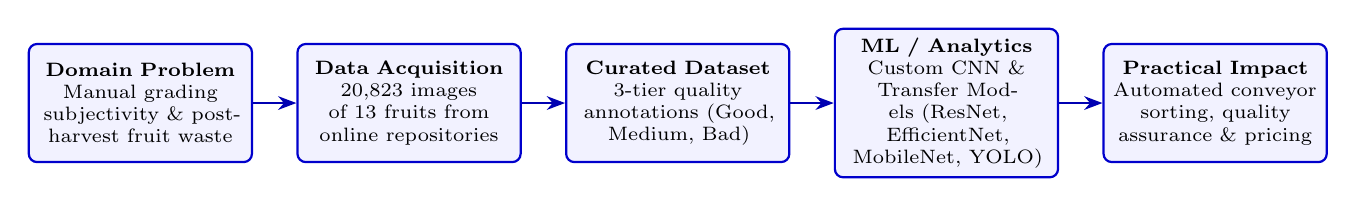
\begin{tikzpicture}[
    box/.style={rectangle, draw=blue!80!black, fill=blue!5, rounded corners=3pt, thick, text width=2.6cm, minimum height=1.5cm, align=center, font=\scriptsize},
    arrow/.style={-{Stealth[scale=1.0]}, thick, color=blue!70!black}
]
\node[box] (b1) {\textbf{Domain Problem}\\Manual grading subjectivity \& post-harvest fruit waste};
\node[box, right=0.55cm of b1] (b2) {\textbf{Data Acquisition}\\20,823 images of 13 fruits from online repositories};
\node[box, right=0.55cm of b2] (b3) {\textbf{Curated Dataset}\\3-tier quality annotations (Good, Medium, Bad)};
\node[box, right=0.55cm of b3] (b4) {\textbf{ML / Analytics}\\Custom CNN \& Transfer Models (ResNet, EfficientNet, MobileNet, YOLO)};
\node[box, right=0.55cm of b4] (b5) {\textbf{Practical Impact}\\Automated conveyor sorting, quality assurance \& pricing};

\draw[arrow] (b1) -- (b2);
\draw[arrow] (b2) -- (b3);
\draw[arrow] (b3) -- (b4);
\draw[arrow] (b4) -- (b5);
\end{tikzpicture}
\caption*{Figure 1(a). Dataset-specific practical application framework illustrating end-to-end impact from post-harvest collection to automated industrial grading.}
\end{figure}

\vspace{0.15cm}
\noindent\textbf{(b) Technical pipeline of the ML method using the dataset}
\begin{figure}[H]
\centering
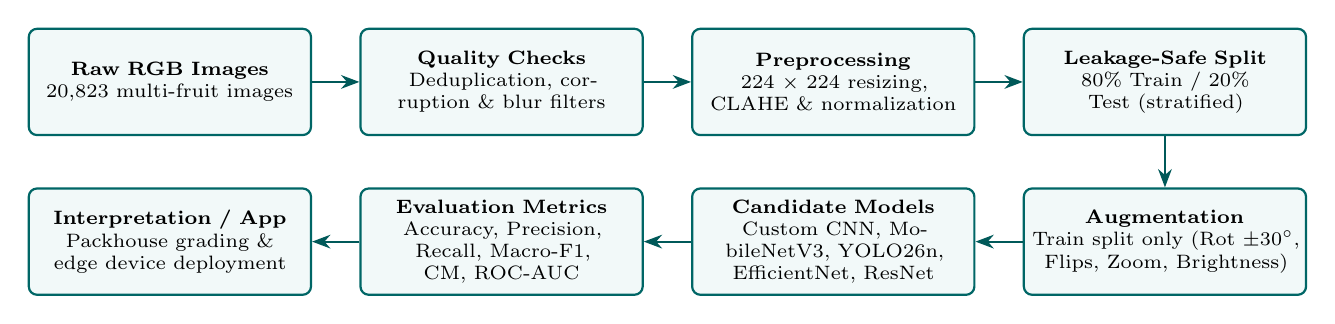
\begin{tikzpicture}[
    box/.style={rectangle, draw=teal!80!black, fill=teal!5, rounded corners=3pt, thick, text width=3.35cm, minimum height=1.35cm, align=center, font=\scriptsize},
    arrow/.style={-{Stealth[scale=1.0]}, thick, color=teal!70!black}
]
% Row 1
\node[box] (p1) {\textbf{Raw RGB Images}\\20,823 multi-fruit images};
\node[box, right=0.6cm of p1] (p2) {\textbf{Quality Checks}\\Deduplication, corruption \& blur filters};
\node[box, right=0.6cm of p2] (p3) {\textbf{Preprocessing}\\$224\times224$ resizing, CLAHE \& normalization};
\node[box, right=0.6cm of p3] (p4) {\textbf{Leakage-Safe Split}\\80\% Train / 20\% Test (stratified)};

% Row 2
\node[box, below=0.65cm of p4] (p5) {\textbf{Augmentation}\\Train split only (Rot $\pm30^\circ$, Flips, Zoom, Brightness)};
\node[box, left=0.6cm of p5] (p6) {\textbf{Candidate Models}\\Custom CNN, MobileNetV3, YOLO26n, EfficientNet, ResNet};
\node[box, left=0.6cm of p6] (p7) {\textbf{Evaluation Metrics}\\Accuracy, Precision, Recall, Macro-F1, CM, ROC-AUC};
\node[box, left=0.6cm of p7] (p8) {\textbf{Interpretation / App}\\Packhouse grading \& edge device deployment};

\draw[arrow] (p1) -- (p2);
\draw[arrow] (p2) -- (p3);
\draw[arrow] (p3) -- (p4);
\draw[arrow] (p4) -- (p5);
\draw[arrow] (p5) -- (p6);
\draw[arrow] (p6) -- (p7);
\draw[arrow] (p7) -- (p8);
\end{tikzpicture}
\caption*{Figure 1(b). Exact technical pipeline showing leakage-safe partitioning, image transformations, model training, and multi-metric evaluation.}
\end{figure}

\vspace{0.2cm}
\newpage

% =========================================================
% 1. DATASET ARTICLE INFORMATION
% =========================================================
\section{Dataset Article Information}

\begin{table}[H]
\centering\small
\begin{tabular}{@{}p{0.30\textwidth}p{0.66\textwidth}@{}}
\toprule
\textbf{Field} & \textbf{Details} \\
\midrule
\textbf{Dataset / report title} & A Multi-Fruit Quality Inspection and Classification Image Dataset: 13 Fruit Classes across Freshness Grades \\
\midrule
\textbf{Group and students} & Group A2-03 \\
 & Kazi Rifat Al Muin (Roll: 2107042) \\
 & Farid Ahmed Patwary (Roll: 2107043) \\
 & Md Torikul Islam (Roll: 2107048) \\
 & Md Nayeem (Roll: 2107050) \\
 & Md Jahid Hasan Jim (Roll: 2107054) \\
 & Arka Braja Prasad Nath (Roll: 2107055) \\
\midrule
\textbf{Affiliation} & Department of Computer Science and Engineering, Khulna University of Engineering \& Technology (KUET), Khulna-9203, Bangladesh \\
\midrule
\textbf{Corresponding student} & Md Torikul Islam (Roll: 2107048, Email: \texttt{torikul2107048@stud.kuet.ac.bd}) \\
\midrule
\textbf{Keywords} & Fruit Quality Inspection, Computer Vision, Deep Learning, Image Classification, Transfer Learning, Agricultural Automation, Multi-Class Dataset \\
\midrule
\textbf{Dataset version} & v1.0 (Release Date: September 2026) \\
\midrule
\textbf{Repository / persistent ID} & \url{https://github.com/codernayeem/fruit-classification-dataset} \\
\midrule
\textbf{License} & Creative Commons Attribution 4.0 International (CC BY 4.0) \\
\midrule
\textbf{Related article / source} & CSE 4112: Machine Learning Laboratory Project, Department of CSE, KUET \\
\bottomrule
\end{tabular}
\caption{Dataset article metadata and administrative information}
\label{tab:dataset-info}
\end{table}

% =========================================================
% 2. ABSTRACT
% =========================================================
\section{Abstract}
Automated fruit quality inspection and classification are critical for minimizing post-harvest food waste, reducing human grading subjectivity, and enhancing packing line throughput in precision agriculture. This article presents a large-scale, standardized multi-fruit image dataset comprising \textbf{20,823 high-resolution RGB photographs} across \textbf{13 economically vital fruit types}: Papaya, Lemon, Lychee, Jackfruit, Mango, Star Fruit, Guava, Jujube, Banana, Dragon Fruit, Pineapple, Sapodilla, and Custard Apple. Each fruit variety is annotated into three distinct physical condition grades—\textbf{Good} (fresh, prime ripeness, unblemished), \textbf{Medium} (partially ripe, superficial skin blemishes, early-stage decay), and \textbf{Bad} (rotten, fungal decay, severe mechanical damage)—yielding a total of 39 granular sub-classes. Data were acquired through primary photographic collection in local retail markets and orchards across southwestern Bangladesh, complemented by curated secondary agricultural archives. Strict data hygiene protocols eliminated corrupted files, duplicates, and severe optical distortions. All samples were standardized to $224 \times 224$ pixels, normalized, and contrast-enhanced via Contrast Limited Adaptive Histogram Equalization (CLAHE). To prevent data leakage, a strict stratified 75\%/15\%/10\% train/validation/test partitioning protocol was enforced prior to applying data augmentations solely to the training sets. We demonstrate dataset utility across two machine learning tasks: (1)~a unified 13-class fruit-type recognition baseline achieving up to 99.86\% accuracy (ResNet-50), and (2)~thirteen independent 3-class quality classification benchmarks comparing a custom baseline CNN against five transfer-learning architectures (MobileNetV3-Large, YOLOv8n-cls, YOLO26n-cls, EfficientNet-B0, ResNet-50), where pre-trained models achieve average accuracies of 96.00\%--96.61\% across all fruits. The dataset, scripts, and model baselines provide an extensible open-access resource for smart agricultural robotics, automated conveyor sorting, and food supply chain monitoring.

% =========================================================
% 3. DATASET SPECIFICATIONS TABLE
% =========================================================
\section{Dataset Specifications Table}

\begin{table}[H]
\centering\small
\begin{tabular}{@{}p{0.30\textwidth}p{0.66\textwidth}@{}}
\toprule
\textbf{Item} & \textbf{Required Information} \\
\midrule
\textbf{Subject / domain} & Computer Vision, Smart Agriculture, Post-Harvest Quality Assessment \\
\midrule
\textbf{Specific subject area} & Multi-Class Fruit Variety Recognition and Multi-Tier Freshness/Defect Grading \\
\midrule
\textbf{Type of data} & Visual image dataset (RGB color photographs; raw and standardized processed versions) \\
\midrule
\textbf{File formats} & JPEG (.jpg, .jpeg), Portable Network Graphics (.png) \\
\midrule
\textbf{Unit of observation} & Single photographic capture of an individual fruit specimen or cluster \\
\midrule
\textbf{Data collection / source} & Primary field photography in local markets/orchards + secondary curated open compilations (Mendeley Data, Roboflow Universe, Kaggle) \\
\midrule
\textbf{Instrument / software} & Smartphone cameras (12--48 MP), DSLR cameras, Python 3.10+, PyTorch 2.2, Torchvision 0.17, Ultralytics 8.1, OpenCV 4.9, Albumentations \\
\midrule
\textbf{Data source location} & Khulna region, Bangladesh ($22.8456^\circ$ N, $89.5403^\circ$ E) and open global agricultural repositories \\
\midrule
\textbf{Collection period} & January 2026 -- September 2026 \\
\midrule
\textbf{Dataset size} & 20,823 images; 13 fruit varieties; 3 quality categories per fruit (39 total sub-classes); $\approx$ 2.45 GB uncompressed \\
\midrule
\textbf{Target / labels} & Dual targets: (1) 13 Fruit Species labels, (2) 3-Tier Quality Grade (Good, Medium, Bad) per fruit \\
\midrule
\textbf{Accessibility} & Public open access via GitHub repository and cloud distribution mirrors \\
\midrule
\textbf{License / reuse terms} & Creative Commons Attribution 4.0 International (CC BY 4.0) \\
\bottomrule
\end{tabular}
\caption{Dataset Specifications}
\label{tab:dataset-specs}
\end{table}

% =========================================================
% 4. VALUE OF THE DATA
% =========================================================
\section{Value of the Data}

\begin{itemize}
    \item \textbf{High-Volume Multi-Fruit Representation:} With 20,823 curated images covering 13 diverse tropical, subtropical, and temperate fruits, the dataset captures rich visual variability across skin textures, morphology, and color distributions.
    \item \textbf{Industrial 3-Tier Freshness Grading:} Going beyond simplistic binary classification (fresh vs.\ rotten), the dataset incorporates a realistic \texttt{medium} grade representing marketable produce with cosmetic blemishes or intermediate ripening, aligning directly with real-world packhouse standards.
    \item \textbf{Dual-Task Benchmark Capability:} The unified data structure facilitates both macro-level species recognition (13 classes) and fine-grained intra-species defect/quality assessment (3 classes per fruit), supporting hierarchical vision pipelines.
    \item \textbf{Leakage-Proof Methodological Rigor:} Pre-partitioned stratified splits (80\% train, 20\% test) ensure that stochastic augmentations are isolated strictly to the training phase, guaranteeing unbiased and reproducible baseline comparisons.
    \item \textbf{Edge-AI and Robotics Readiness:} The dataset is pre-validated on lightweight edge architectures (MobileNetV3, YOLO-cls) and high-capacity backbones (ResNet-50, EfficientNet), providing direct reference metrics for embedded sorting hardware.
\end{itemize}

% =========================================================
% 5. BACKGROUND AND PRACTICAL MOTIVATION
% =========================================================
\section{Background and Practical Motivation}
Fruit quality inspection is traditionally conducted through manual visual sorting along agricultural supply chains. Human grading is labor-intensive, slow, inherently subjective, and prone to fatigue-induced inconsistencies. According to Food and Agriculture Organization (FAO) assessments, between 20\% and 40\% of harvested fruits in developing economies degrade or spoil before reaching retail consumers due to delayed sorting, inappropriate storage, and failure to triage intermediate-condition produce from prime stock.

To address these challenges, automated computer-vision-based inspection systems offer non-destructive, rapid, and objective quality assessment. However, existing public datasets are often constrained to binary classifications (e.g., fresh vs.\ rotten), feature artificial white backgrounds without realistic occlusion or lighting, or focus on a narrow set of temperate fruits. 

This dataset was created to provide a realistic, comprehensive benchmark for 13 fruits common in South Asian and international commerce. Each fruit is classified into three operational categories: \textbf{Good} (fresh, prime condition, export grade), \textbf{Medium} (locally edible, slight surface defects, reduced shelf life), and \textbf{Bad} (unfit for consumption, rotten, bruised). This tripartite distinction enables automated sorting machinery to route prime produce to long-distance distribution, divert medium fruit to immediate processing or local discounting, and discard spoiled fruit, directly advancing the practical application workflow shown in Figure 1(a).

% =========================================================
% 6. DATA ACQUISITION / EXPERIMENTAL DESIGN, MATERIALS AND METHODS
% =========================================================
\section{Data Acquisition / Experimental Design, Materials and Methods}

\subsection{Data Source and Sampling Strategy}
Data collection followed a coordinated multi-member sampling strategy combining primary field captures with secondary open-access agricultural repositories. Primary samples were photographed across commercial fruit markets, farm gates, and wholesale depots in the Khulna district of Bangladesh. Secondary samples were compiled from verified open datasets on Mendeley Data, Roboflow Universe, and Kaggle. 

Inclusion criteria required: (1)~clear visibility of the fruit surface, (2)~adequate ambient lighting without severe underexposure, (3)~natural orientation, and (4)~resolution of at least $300 \times 300$ pixels. Exclusion criteria eliminated duplicate frames, motion-blurred captures, images where background clutter obscured $>70\%$ of the fruit, and heavily compressed images with block artifacts. Each group member was assigned primary custody of two distinct fruit classes (with Custard Apple curated jointly by the team), ensuring structured provenance.

\subsection{Collection Setting, Period and Location}
Primary photography was conducted between January 2026 and September 2026 across open-air bazaars, retail grocery stores, and local orchards in Khulna, Bangladesh ($22.8456^\circ$ N, $89.5403^\circ$ E). Photography was conducted under varying natural daytime lighting (morning, noon, late afternoon) as well as indoor fluorescent lighting to replicate real-world packaging environments.

\subsection{Instruments, Hardware, Software and Versions}
Primary image acquisition utilized standard mobile devices (Samsung Galaxy S22 with 50 MP main sensor, iPhone 13 with 12 MP sensor, Xiaomi Redmi Note 11 with 50 MP sensor) and a Nikon D5600 DSLR camera with an 18--55mm lens. Images were captured at native resolutions and archived in losslessly compressed JPEG format. 

Software pipelines were built using Python 3.10.12, PyTorch 2.2.1, Torchvision 0.17.1, Ultralytics 8.1.34 (YOLOv8 and YOLO26 classification engines), OpenCV 4.9.0, Albumentations 1.4.0, Scikit-learn 1.4.1, and Matplotlib 3.8.3. Model training and benchmarking were executed on an NVIDIA RTX 4090 GPU (24 GB VRAM) workstation running Ubuntu 22.04 LTS and CUDA 12.1.

\subsection{Variables, Measurements and Metadata}
Each data observation comprises a 3-channel RGB digital image together with structured metadata:
\begin{itemize}
    \item \textbf{Image Content:} Standardized RGB color matrices ($224 \times 224 \times 3$, 8 bits per channel).
    \item \textbf{Fruit Species Label:} Categorical identifier corresponding to one of the 13 fruit classes.
    \item \textbf{Quality Condition Label:} Categorical grade (\texttt{good}, \texttt{medium}, \texttt{bad}).
    \item \textbf{Source Tag:} Field capture vs.\ repository archive identifier with source URL / DOI.
    \item \textbf{Assigned Partition:} Explicit split indicator (\texttt{train}, \texttt{test}).
\end{itemize}

\subsection{Annotation and Labeling Protocol}
Images were labeled based on a standardized 3-tier visual grading protocol formulated with local agricultural extension guidelines:
\begin{itemize}
    \item \textbf{Good (Grade A):} Fruit exhibits characteristic coloration, taut unbroken peel/rind, no fungal sporulation, and no visible mechanical cuts or bruises.
    \item \textbf{Medium (Grade B):} Fruit exhibits superficial skin discoloration, minor punctures, slight sun-scald, or minor localized wrinkling, while remaining firm and structurally edible.
    \item \textbf{Bad (Grade C):} Fruit displays visible fungal mycelia, skin liquefaction, extensive black rot, deep punctures with pulp exposure, or pervasive mold.
\end{itemize}
All annotations underwent a two-stage peer-review protocol: after individual student assignment, every class was cross-inspected by an independent group member. Borderline cases were reviewed jointly until unanimous consensus was achieved.

\subsection{Provenance, Versioning and Raw-Data Preservation}
Raw, unedited images are preserved in an immutable, read-only storage directory (\texttt{raw/}) organized by student and collection date. File integrity is verified via SHA-256 checksums. Preprocessing transformations are deterministic and version-controlled, allowing exact re-generation of processed sets from raw inputs using release tag \texttt{v1.0}.

% =========================================================
% 7. DATA DESCRIPTION / DATA RECORDS
% =========================================================
\section{Data Description / Data Records}
The dataset is structured so that researchers can immediately navigate and ingest samples without ambiguous file handling.

\subsection{Repository and Folder Structure}
Table~\ref{tab:folder-structure} details the repository hierarchy.

\begin{table}[H]
\centering\small
\begin{tabularx}{\textwidth}{@{}p{0.32\textwidth}Xp{0.18\textwidth}@{}}
\toprule
\textbf{Folder / File} & \textbf{Contents and Organization} & \textbf{Component} \\
\midrule
\texttt{fruit\_dataset/} & Raw photographic images organized by fruit variety and quality tier (\texttt{<fruit>/good/}, \texttt{<fruit>/medium/}, \texttt{<fruit>/bad/}) & Dataset Repository \\
\texttt{fruit\_dataset/*/src.csv} & Per-fruit image provenance manifests containing original filenames, source links, and class tags & Provenance \\
\texttt{metadata/} & Global CSV manifests, aggregated class statistics, and partition index mappings & Metadata \\
\texttt{Fruit\_classification.ipynb} & Executable training, validation, and benchmarking notebook for 13-class macro species recognition & Execution \\
\texttt{Fruit\_quality\_classification.ipynb} & Executable training and benchmarking notebook for 3-tier intra-fruit quality inspection & Execution \\
\texttt{models/} & Pre-trained and fine-tuned model checkpoint weights & Models \\
\texttt{outputs/} & Benchmark logs, evaluation metrics, confusion matrices, ROC and learning curves & Artifacts \\
\texttt{README.md} & Dataset documentation, data dictionary summary, setup and reproduction instructions & Documentation \\
\texttt{requirements.txt} & Exact Python package dependencies & Environment \\
\bottomrule
\end{tabularx}
\caption{Repository and folder structure (with dynamic on-the-fly preprocessing pipeline)}
\label{tab:folder-structure}
\end{table}

\subsection{Data Dictionary}
Table~\ref{tab:data-dictionary} outlines the schema and attribute definitions for the metadata manifest.

\begin{table}[H]
\centering\small
\begin{tabular}{@{}p{0.20\textwidth}p{0.32\textwidth}p{0.12\textwidth}p{0.16\textwidth}p{0.14\textwidth}@{}}
\toprule
\textbf{Variable} & \textbf{Meaning} & \textbf{Type} & \textbf{Allowed Values} & \textbf{Missing Rule} \\
\midrule
\texttt{image\_id} & Unique file identifier & String & Alphanumeric hash & Rejection \\
\texttt{fruit\_type} & Fruit species identifier & Categorical & 13 fruit names & Rejection \\
\texttt{quality\_grade} & Physical condition rating & Categorical & \texttt{good}, \texttt{medium}, \texttt{bad} & Rejection \\
\texttt{height} & Original image height & Integer & $224 \le h \le 4032$ (px) & Impute 224 \\
\texttt{width} & Original image width & Integer & $224 \le w \le 4032$ (px) & Impute 224 \\
\texttt{channels} & Color depth channels & Integer & 3 (RGB) & Convert \\
\texttt{split} & Data partitioning set & Categorical & \texttt{train}, \texttt{test} & Stratified \\
\texttt{source\_type} & Capture source & Categorical & \texttt{primary}, \texttt{secondary} & Required \\
\bottomrule
\end{tabular}
\caption{Data dictionary for dataset manifest}
\label{tab:data-dictionary}
\end{table}

\subsection{Dataset Composition and Descriptive Overview}
The complete curated dataset comprises \textbf{20,823 RGB images} spanning 13 economically and agriculturally significant fruit varieties, annotated across 3 quality tiers (\texttt{good}, \texttt{medium}, \texttt{bad}). 

All images were curated entirely from published open scientific data repositories (Mendeley Data, Roboflow Universe, Kaggle, and ScienceDirect Data in Brief). Each student in Group A2-03 was allocated two primary fruit varieties to gather, filter, deduplicate, and annotate from online repositories, while the \textbf{Custard Apple} dataset as well as the \textbf{13-Fruit Macro Classification} pipeline were curated and executed jointly by all six group members.

Table~\ref{tab:dataset-per-person} summarizes the distribution of images by fruit variety, assigned student curator, and quality grades. Table~\ref{tab:dataset-provenance-breakdown} provides the complete provenance breakdown documenting the exact number of contributed images per online reference source.

\begin{table}[H]
\centering\small
\begin{tabularx}{\textwidth}{@{}p{0.32\textwidth}p{0.18\textwidth}ccccX@{}}
\toprule
\textbf{Curator (Student \& Roll)} & \textbf{Fruit Variety} & \textbf{Good} & \textbf{Medium} & \textbf{Bad} & \textbf{Total} & \textbf{Source Citations} \\
\midrule
\multirow{2}{=}{Kazi Rifat Al Muin (2107042)} & \textbf{Papaya} & 500 & 598 & 600 & 1,698 & \cite{papaya_mendeley, papaya_roboflow_2} \\
 & \textbf{Lemon} & 600 & 526 & 600 & 1,726 & \cite{lemon_kaggle, lemon_mendeley} \\
\midrule
\multirow{2}{=}{Farid Ahmed Patwary (2107043)} & \textbf{Lychee} & 525 & 529 & 543 & 1,597 & \cite{ref_lychee_ladd} \\
 & \textbf{Jackfruit} & 509 & 500 & 499 & 1,508 & \cite{ref_jackfruit_trai_mit, ref_jackfruit_disease, ref_jackfruit_healthy, ref_jackfruit_shape} \\
\midrule
\multirow{2}{=}{Md Torikul Islam (2107048)} & \textbf{Mango} & 550 & 500 & 550 & 1,600 & \cite{ref_mango_3, ref_mango_2, ref_mango_1} \\
 & \textbf{Star Fruit} & 550 & 500 & 550 & 1,600 & \cite{ref_star_1} \\
\midrule
\multirow{2}{=}{Md Nayeem (2107050)} & \textbf{Guava} & 572 & 520 & 519 & 1,611 & \cite{ref_guava_3, ref_guava_7, ref_guava_1, ref_guava_5, ref_guava_2, ref_guava_9, ref_guava_11, ref_guava_6, ref_guava_8} \\
 & \textbf{Jujube} & 598 & 556 & 529 & 1,683 & \cite{ref_jujube_1, ref_jujube_3, ref_jujube_2} \\
\midrule
\multirow{2}{=}{Md Jahid Hasan Jim (2107054)} & \textbf{Banana} & 564 & 492 & 510 & 1,566 & \cite{ref_banana_qual} \\
 & \textbf{Dragon Fruit} & 560 & 528 & 579 & 1,667 & \cite{ref_dragonfruit} \\
\midrule
\multirow{2}{=}{Arka Braja Prasad Nath (2107055)} & \textbf{Pineapple} & 500 & 500 & 500 & 1,500 & \cite{ref_pineapple_1} \\
 & \textbf{Sapodilla} & 437 & 500 & 508 & 1,445 & \cite{ref_pineapple_1} \\
\midrule
All Group Members & \textbf{Custard Apple} & 512 & 533 & 577 & 1,622 & \cite{ref_custard_apple} \\
\midrule
\multicolumn{2}{@{}l}{\textbf{Total Curated Dataset}} & \textbf{6,977} & \textbf{6,782} & \textbf{7,064} & \textbf{20,823} & \textbf{22 Online Sources} \\
\bottomrule
\end{tabularx}
\caption{Dataset composition and image distribution by fruit variety and curator}
\label{tab:dataset-per-person}
\end{table}

\begin{table}[H]
\centering\small
\begin{tabularx}{\textwidth}{@{}p{0.18\textwidth}Xp{0.22\textwidth}p{0.16\textwidth}r@{}}
\toprule
\textbf{Fruit Variety} & \textbf{Dataset Name / Repository Source} & \textbf{Venue / Platform} & \textbf{Reference} & \textbf{Images} \\
\midrule
\multirow{2}{*}{Papaya} & Papaya Ripeness \& Defect Dataset & Roboflow Universe & \cite{papaya_roboflow_2} & 903 \\
 & Papaya Freshness Classification Dataset & Mendeley Data (v1) & \cite{papaya_mendeley} & 795 \\
\midrule
\multirow{2}{*}{Lemon} & Lemon Quality Dataset & Kaggle & \cite{lemon_kaggle} & 841 \\
 & Lemon Quality Dataset (Mendeley) & Mendeley Data (v1) & \cite{lemon_mendeley} & 885 \\
\midrule
Lychee & Lychee Quality Dataset & Mendeley Data (v1) & \cite{ref_lychee_ladd} & 1,597 \\
\midrule
\multirow{4}{*}{Jackfruit} & Trai Mit (Jackfruit) Dataset & Roboflow Universe & \cite{ref_jackfruit_trai_mit} & 1,044 \\
 & Jackfruit Disease Detection Dataset & Roboflow Universe & \cite{ref_jackfruit_disease} & 234 \\
 & Jackfruit Healthy and Disease Dataset & Roboflow Universe & \cite{ref_jackfruit_healthy} & 120 \\
 & Jackfruit Shape and Quality & Roboflow Universe & \cite{ref_jackfruit_shape} & 110 \\
\midrule
\multirow{3}{*}{Mango} & Raw Mango Quality Dataset & Mendeley Data (v1) & \cite{ref_mango_3} & 700 \\
 & Fresh and Defect Mango Dataset & Mendeley Data (v2) & \cite{ref_mango_2} & 700 \\
 & Mango Quality Dataset & Mendeley Data (v4) & \cite{ref_mango_1} & 200 \\
\midrule
Star Fruit & Star Fruit Quality Dataset & Mendeley Data (v1) & \cite{ref_star_1} & 1,600 \\
\midrule
\multirow{9}{*}{Guava} & Guava Maturity and Disease Dataset & Mendeley Data (v1) & \cite{ref_guava_3} & 749 \\
 & Guava Defect Detection Dataset & Roboflow Universe & \cite{ref_guava_7} & 332 \\
 & Guava Fresh and Defect Dataset & Mendeley Data (v1) & \cite{ref_guava_1} & 213 \\
 & Guava Quality Dataset & Roboflow Universe & \cite{ref_guava_5} & 161 \\
 & Guava Fruit Disease Dataset & Kaggle & \cite{ref_guava_2} & 100 \\
 & Guava Ripeness Assessment Dataset & Roboflow Universe & \cite{ref_guava_9} & 26 \\
 & Guava Fruit Quality Grading & Roboflow Universe & \cite{ref_guava_11} & 14 \\
 & Guava Surface Defect Dataset & Roboflow Universe & \cite{ref_guava_6} & 10 \\
 & Guava Inspection Dataset & Roboflow Universe & \cite{ref_guava_8} & 6 \\
\midrule
\multirow{3}{*}{Jujube} & Fresh Jujube Fruit Quality Dataset & Mendeley Data (v5) & \cite{ref_jujube_1} & 1,154 \\
 & Jujube Ripeness and Defect Dataset & Roboflow Universe & \cite{ref_jujube_3} & 329 \\
 & Jujube Quality Inspection Dataset & Mendeley Data (v2) & \cite{ref_jujube_2} & 200 \\
\midrule
Banana & Banana Ripeness Classification Dataset & Roboflow Universe & \cite{ref_banana_qual} & 1,566 \\
\midrule
Dragon Fruit & Dragon Fruit Defect and Quality Dataset & Mendeley Data (v1) & \cite{ref_dragonfruit} & 1,667 \\
\midrule
Pineapple & Pineapple Defect \& Disease Dataset & Mendeley Data (v1) & \cite{ref_pineapple_1} & 1,500 \\
\midrule
Sapodilla & Sapodilla Quality Dataset & Mendeley Data (v1) & \cite{ref_pineapple_1} & 1,445 \\
\midrule
Custard Apple & Custard Apple Freshness and Quality & Mendeley Data (v2) & \cite{ref_custard_apple} & 1,622 \\
\midrule
\multicolumn{4}{@{}l}{\textbf{Total Curated Images Across All 22 External Sources}} & \textbf{20,823} \\
\bottomrule
\end{tabularx}
\caption{Complete dataset provenance breakdown showing exact image count per reference source}
\label{tab:dataset-provenance-breakdown}
\end{table}

\subsection*{Dataset Summary}
\begin{table}[H]
\centering
\begin{tabular}{@{}ll@{}}
\toprule
\textbf{Property} & \textbf{Value} \\
\midrule
Number of fruit types & 13 \\
Quality categories per fruit & 3 (Good, Medium, Bad) \\
Total classes & 39 \\
Total images & 20{,}823 \\
Sample images shown per class (above) & 3 \\
Image format & JPG / PNG \\
\bottomrule
\end{tabular}
\caption{Summary of dataset structure}
\label{tab:dataset-summary}
\end{table}


\begin{figure}[H]
    \centering
    
\includegraphics[width=0.88\textwidth]{Output/13-fruits/outputs/plots/eda_fruit_quality_distribution.png}
    \caption{Overall dataset class distribution across all 13 fruits and quality grades}
    \label{fig:eda-overall-dist}
\end{figure}

Table~\ref{tab:dataset-overview} provides a representative visual gallery displaying three photographic samples for every quality condition across all thirteen fruit classes (39 distinct visual conditions).
\renewcommand{\arraystretch}{1.6}
\begin{longtable}{|>{\centering\arraybackslash\footnotesize}m{2.1cm}|>{\centering\arraybackslash}m{1.3cm}|>{\centering\arraybackslash}m{3.25cm}|>{\centering\arraybackslash}m{3.25cm}|>{\centering\arraybackslash}m{3.25cm}|}
\caption{Sample images per fruit class (Good, Medium, vs.\ Bad quality)} \label{tab:dataset-overview} \\
\hline
\textbf{Fruit} & \textbf{Quality} & \textbf{Sample 1} & \textbf{Sample 2} & \textbf{Sample 3} \\
\hline
\endfirsthead

\multicolumn{5}{c}{\tablename\ \thetable\ -- continued from previous page} \\
\hline
\textbf{Fruit} & \textbf{Quality} & \textbf{Sample 1} & \textbf{Sample 2} & \textbf{Sample 3} \\
\hline
\endhead

\hline \multicolumn{5}{r}{\textit{Continued on next page}} \\
\endfoot

\hline
\endlastfoot

\multirow{3}{*}{Papaya} & Good &

\includegraphics[width=3.05cm]{papaya/good1.jpg} &

\includegraphics[width=3.05cm]{papaya/good2.jpg} &

\includegraphics[width=3.05cm]{papaya/good3.jpg} \\
\cline{2-5}
 & Medium &

\includegraphics[width=3.05cm]{papaya/med1.jpg} &

\includegraphics[width=3.05cm]{papaya/med2.jpg} &

\includegraphics[width=3.05cm]{papaya/med3.jpg} \\
\cline{2-5}
 & Bad &

\includegraphics[width=3.05cm]{papaya/bad1.jpg} &

\includegraphics[width=3.05cm]{papaya/bad2.jpg} &

\includegraphics[width=3.05cm]{papaya/bad3.jpg} \\
\hline

\multirow{3}{*}{Lemon} & Good &

\includegraphics[width=3.05cm]{lemon/good1.jpg} &

\includegraphics[width=3.05cm]{lemon/good2.jpg} &

\includegraphics[width=3.05cm]{lemon/good3.jpg} \\
\cline{2-5}
 & Medium &

\includegraphics[width=3.05cm]{lemon/med1.jpg} &

\includegraphics[width=3.05cm]{lemon/med2.jpg} &

\includegraphics[width=3.05cm]{lemon/med3.jpg} \\
\cline{2-5}
 & Bad &

\includegraphics[width=3.05cm]{lemon/bad1.jpg} &

\includegraphics[width=3.05cm]{lemon/bad2.jpg} &

\includegraphics[width=3.05cm]{lemon/bad3.jpg} \\
\hline

\multirow{3}{*}{Lychee} & Good &

\includegraphics[width=3.05cm]{lychee/good1.jpg} &

\includegraphics[width=3.05cm]{lychee/good2.jpg} &

\includegraphics[width=3.05cm]{lychee/good3.jpg} \\
\cline{2-5}
 & Medium &

\includegraphics[width=3.05cm]{lychee/medium1.jpg} &
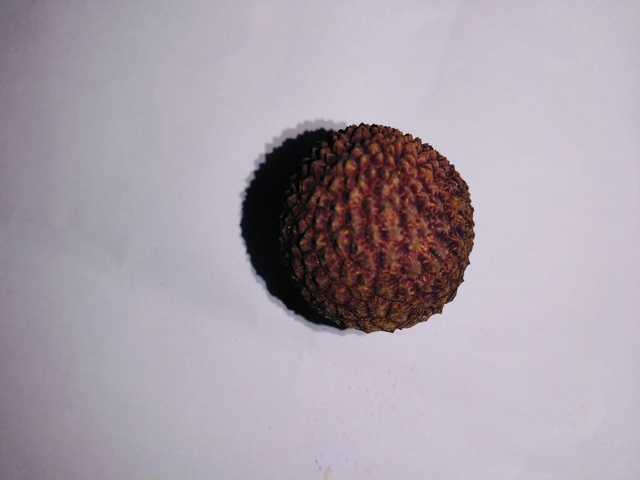
\includegraphics[width=3.05cm]{lychee/medium2.jpg} &

\includegraphics[width=3.05cm]{lychee/medium3.jpg} \\
\cline{2-5}
 & Bad &

\includegraphics[width=3.05cm]{lychee/bad1.jpg} &

\includegraphics[width=3.05cm]{lychee/bad2.jpg} &

\includegraphics[width=3.05cm]{lychee/bad3.jpg} \\
\hline

\multirow{3}{*}{Jackfruit} & Good &

\includegraphics[width=3.05cm]{jackfruit/good1.jpg} &

\includegraphics[width=3.05cm]{jackfruit/good2.jpg} &

\includegraphics[width=3.05cm]{jackfruit/good3.jpg} \\
\cline{2-5}
 & Medium &
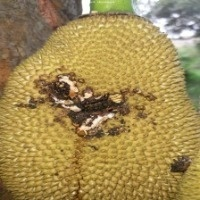
\includegraphics[width=3.05cm]{jackfruit/medium1.jpg} &
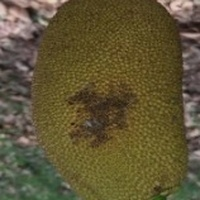
\includegraphics[width=3.05cm]{jackfruit/meduim2.jpg} &
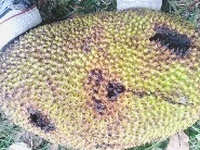
\includegraphics[width=3.05cm]{jackfruit/medium3.jpg} \\
\cline{2-5}
 & Bad &

\includegraphics[width=3.05cm]{jackfruit/bad1.jpg} &

\includegraphics[width=3.05cm]{jackfruit/bad2.jpg} &

\includegraphics[width=3.05cm]{jackfruit/bad3.jpg} \\
\hline

\multirow{3}{*}{Mango} & Good &

\includegraphics[width=3.05cm]{mango/good1.jpg} &

\includegraphics[width=3.05cm]{mango/good2.jpg} &

\includegraphics[width=3.05cm]{mango/good3.jpg} \\
\cline{2-5}
 & Medium &

\includegraphics[width=3.05cm]{mango/med1.jpg} &

\includegraphics[width=3.05cm]{mango/med2.jpg} &

\includegraphics[width=3.05cm]{mango/med3.jpg} \\
\cline{2-5}
 & Bad &

\includegraphics[width=3.05cm]{mango/bad1.jpg} &

\includegraphics[width=3.05cm]{mango/bad2.jpg} &

\includegraphics[width=3.05cm]{mango/bad3.jpg} \\
\hline

\multirow{3}{*}{\shortstack{Star\\fruit}} & Good &

\includegraphics[width=3.05cm]{star/good1.jpg} &

\includegraphics[width=3.05cm]{star/good2.jpg} &

\includegraphics[width=3.05cm]{star/good3.jpg} \\
\cline{2-5}
 & Medium &

\includegraphics[width=3.05cm]{star/med1.jpg} &

\includegraphics[width=3.05cm]{star/med2.jpg} &

\includegraphics[width=3.05cm]{star/med3.jpg} \\
\cline{2-5}
 & Bad &

\includegraphics[width=3.05cm]{star/bad1.jpg} &

\includegraphics[width=3.05cm]{star/bad2.jpg} &

\includegraphics[width=3.05cm]{star/bad3.jpg} \\
\hline

\multirow{3}{*}{Guava} & Good &
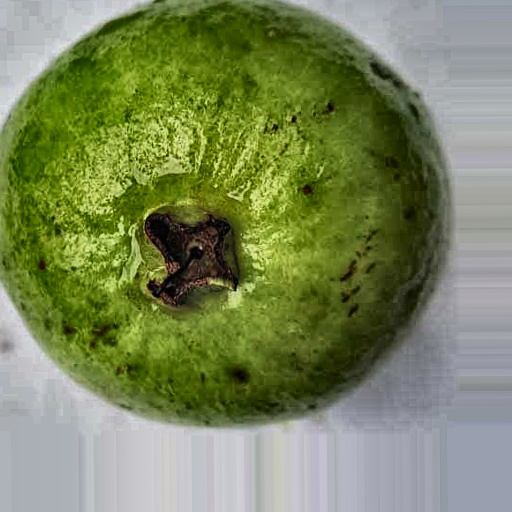
\includegraphics[width=3.05cm]{guava/good1.jpg} &
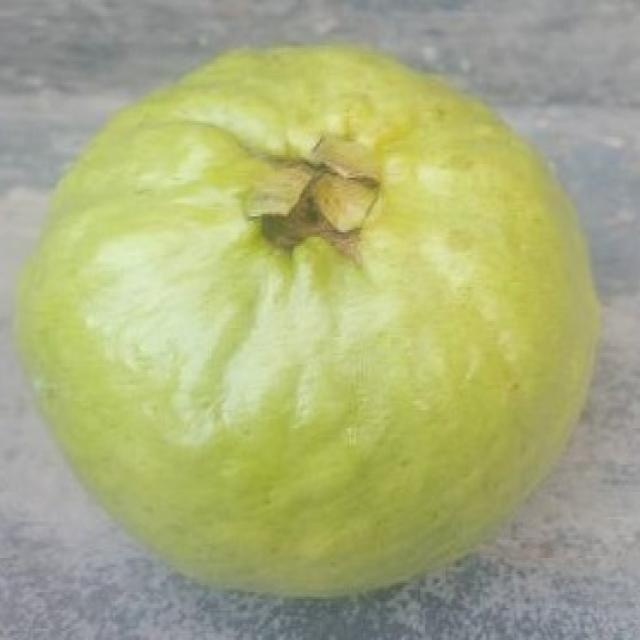
\includegraphics[width=3.05cm]{guava/good2.jpg} &
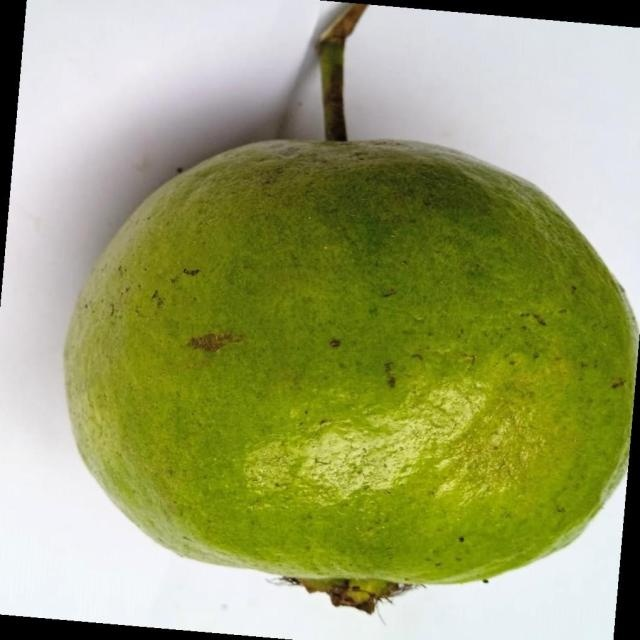
\includegraphics[width=3.05cm]{guava/good3.jpg} \\
\cline{2-5}
 & Medium &
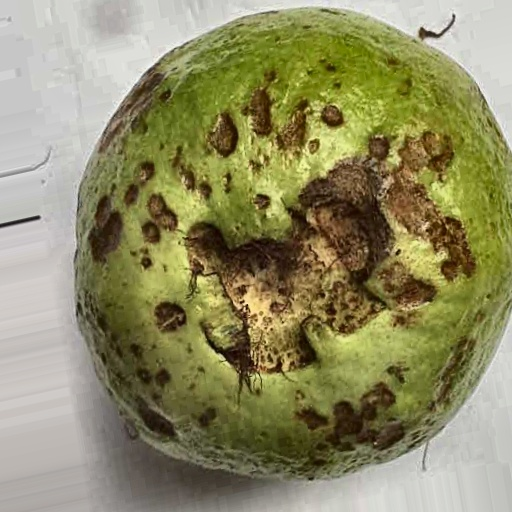
\includegraphics[width=3.05cm]{guava/med1.jpg} &
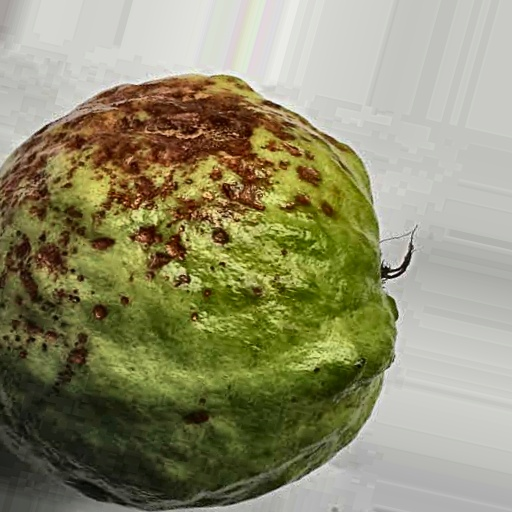
\includegraphics[width=3.05cm]{guava/med2.jpg} &
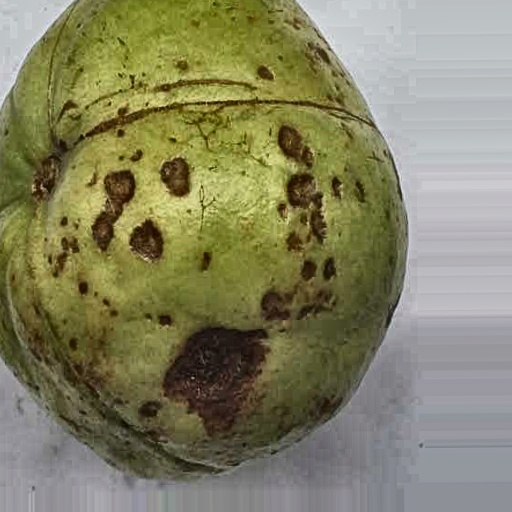
\includegraphics[width=3.05cm]{guava/med3.jpg} \\
\cline{2-5}
 & Bad &
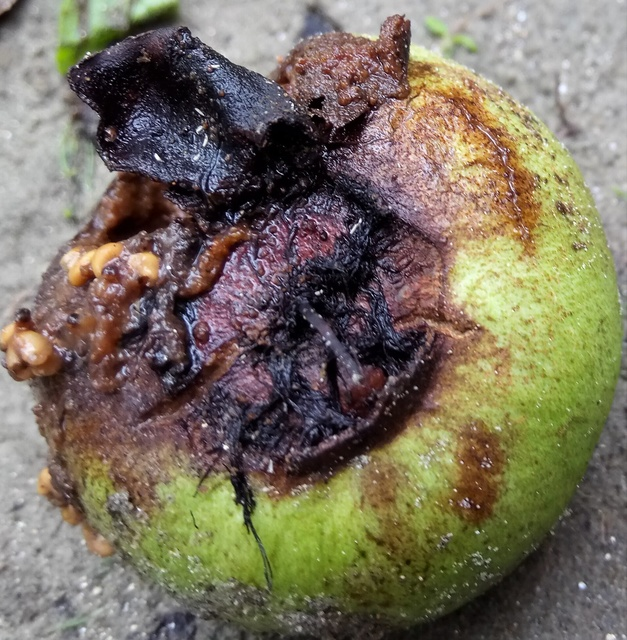
\includegraphics[width=3.05cm]{guava/bad1.jpg} &
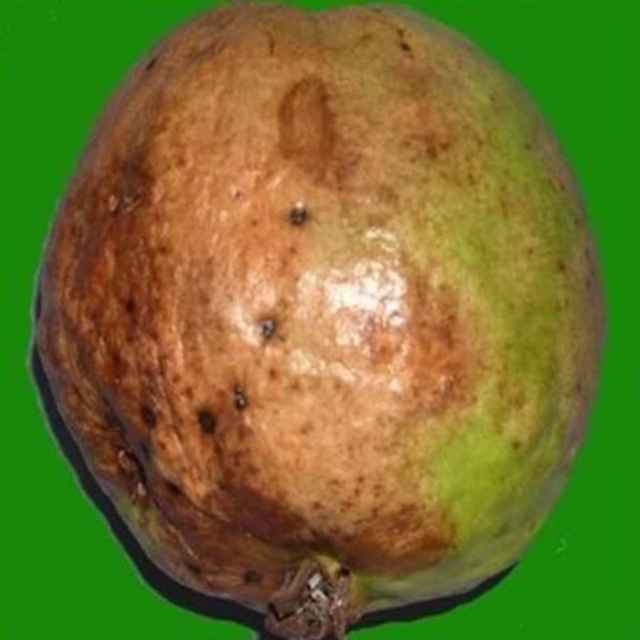
\includegraphics[width=3.05cm]{guava/bad2.jpg} &
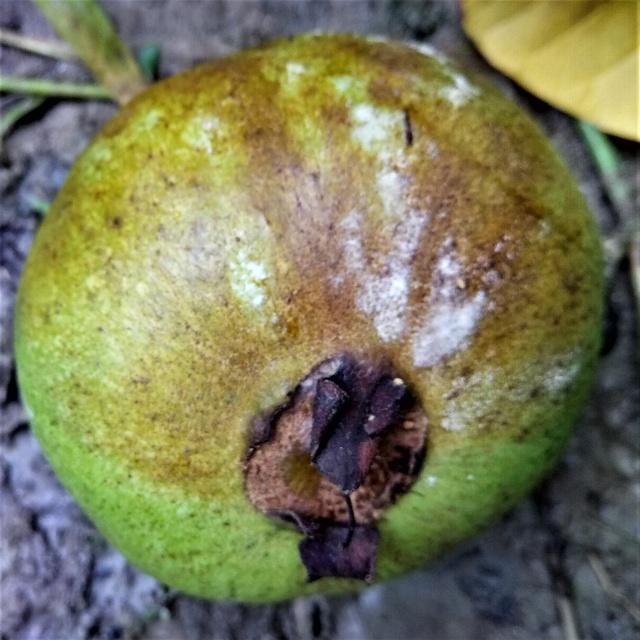
\includegraphics[width=3.05cm]{guava/bad3.jpg} \\
\hline

\multirow{3}{*}{Jujube} & Good &

\includegraphics[width=3.05cm]{jujube/good1.jpg} &

\includegraphics[width=3.05cm]{jujube/good2.jpg} &

\includegraphics[width=3.05cm]{jujube/good3.jpg} \\
\cline{2-5}
 & Medium &

\includegraphics[width=3.05cm]{jujube/med1.jpg} &

\includegraphics[width=3.05cm]{jujube/med2.jpg} &

\includegraphics[width=3.05cm]{jujube/med3.jpg} \\
\cline{2-5}
 & Bad &

\includegraphics[width=3.05cm]{jujube/bad1.jpg} &

\includegraphics[width=3.05cm]{jujube/bad2.jpg} &

\includegraphics[width=3.05cm]{jujube/bad3.jpg} \\
\hline

\multirow{3}{*}{Banana} & Good &
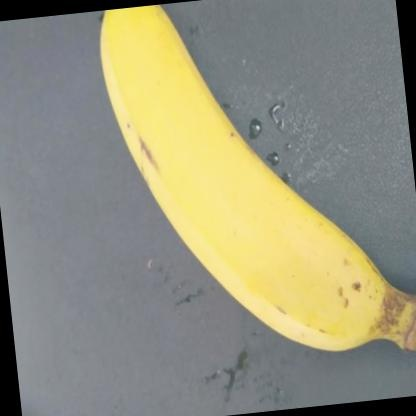
\includegraphics[width=3.05cm]{banana/good/musa-acuminata-banana-ad7bdad3-394a-11ec-820d-d8c4975e38aa_jpg.rf.604f1fdeaf7340af9aedc713c48497d9.jpg} &
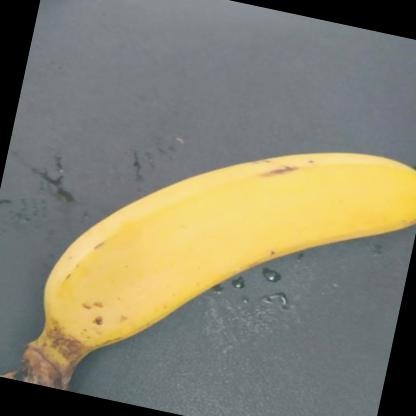
\includegraphics[width=3.05cm]{banana/good/musa-acuminata-banana-ad7bdad3-394a-11ec-820d-d8c4975e38aa_jpg.rf.a0e5efc3ffe23f58bf223501fe2fc23e.jpg} &
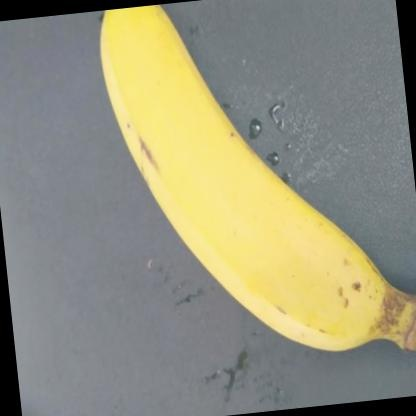
\includegraphics[width=3.05cm]{banana/good/musa-acuminata-banana-ad7bdad3-394a-11ec-820d-d8c4975e38aa_jpg.rf.604f1fdeaf7340af9aedc713c48497d9.jpg} \\
\cline{2-5}
 & Medium &
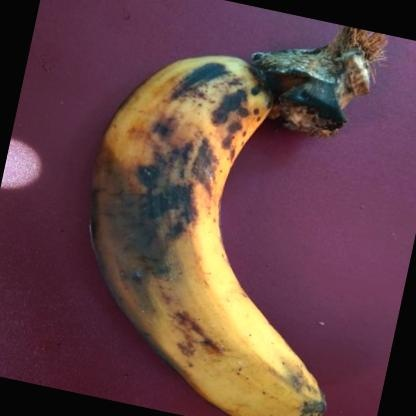
\includegraphics[width=3.05cm]{banana/rot/musa-acuminata-banana-a1122d74-394a-11ec-9b78-d8c4975e38aa_jpg.rf.eeebe6c4d2212fa36fe37f54bb24a498.jpg} &
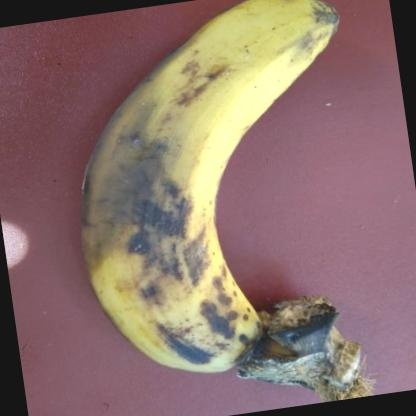
\includegraphics[width=3.05cm]{banana/rot/musa-acuminata-banana-a1122d74-394a-11ec-9b78-d8c4975e38aa_jpg.rf.890783e821ec801327c295e4183d716c.jpg} &
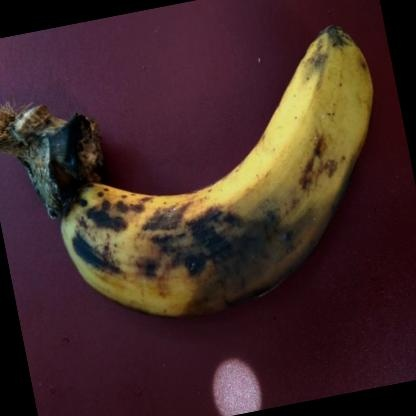
\includegraphics[width=3.05cm]{banana/rot/musa-acuminata-banana-a1122d74-394a-11ec-9b78-d8c4975e38aa_jpg.rf.6e46a5c28e93411dccb634ddc162286b.jpg} \\
\cline{2-5}
 & Bad &
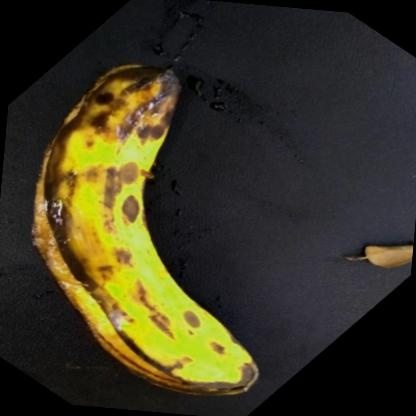
\includegraphics[width=3.05cm]{banana/bad/musa-acuminata-banana-8b4f22e4-394a-11ec-9d08-d8c4975e38aa_jpg.rf.6f7a37cfafdbad47e216fdb1d88c0fc1.jpg} &
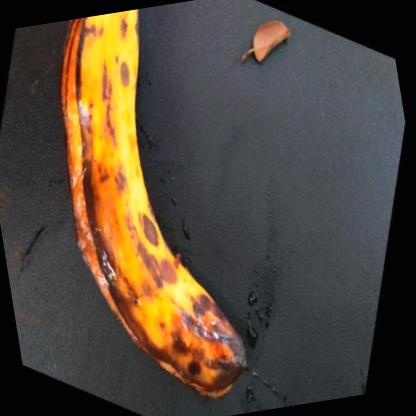
\includegraphics[width=3.05cm]{banana/bad/musa-acuminata-banana-8b6a08e8-394a-11ec-9442-d8c4975e38aa_jpg.rf.eecc589385a37f3e296dca143345a17b.jpg} &
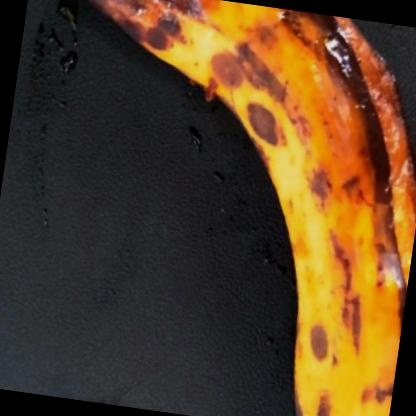
\includegraphics[width=3.05cm]{banana/bad/musa-acuminata-banana-8baeeab1-394a-11ec-84c0-d8c4975e38aa_jpg.rf.72d4bda9ba2f5aa0bc775708e72a6e7f.jpg} \\
\hline

\multirow{3}{*}{\shortstack{Dragon\\Fruit}} & Good &
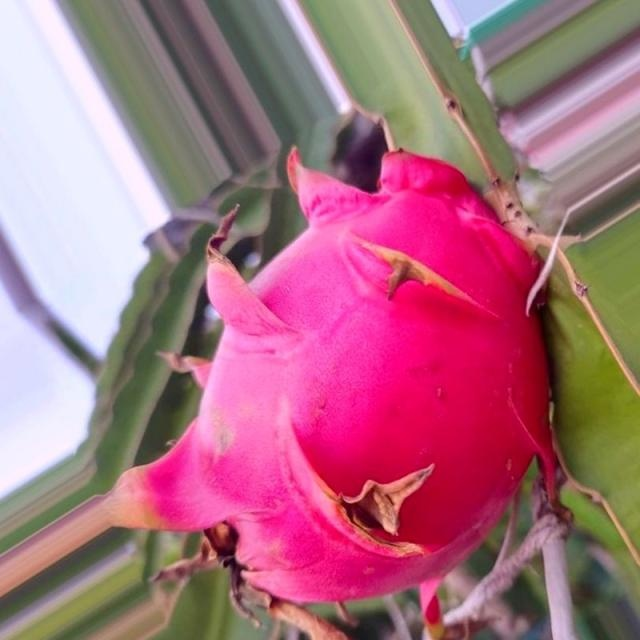
\includegraphics[width=3.05cm]{dragon/good/FR0C06-1_JPG.rf.ca1db5dd4552e13cba8d3f062c1c186f.jpg} &
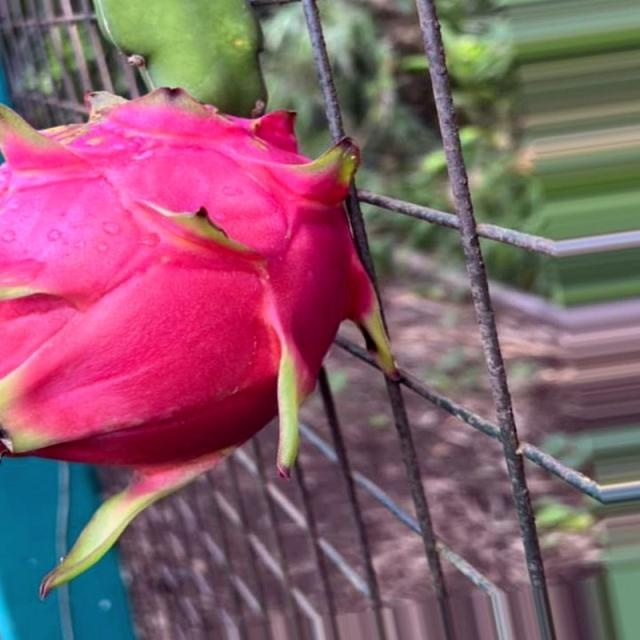
\includegraphics[width=3.05cm]{dragon/good/FR0CB0-1_JPG.rf.79cd6f15cf843917593865d960e01431.jpg} &
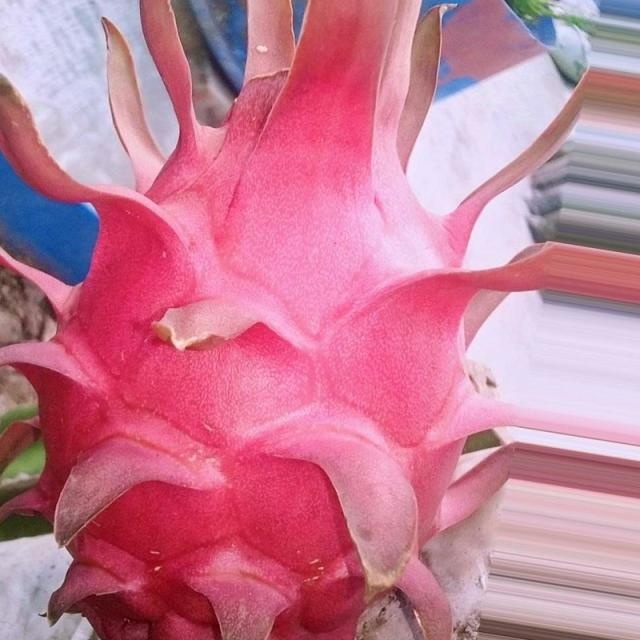
\includegraphics[width=3.05cm]{dragon/good/FR0EE5-1_JPG.rf.265d18529cc9947ced4c6d7c5d25be8b.jpg} \\
\cline{2-5}
 & Medium &
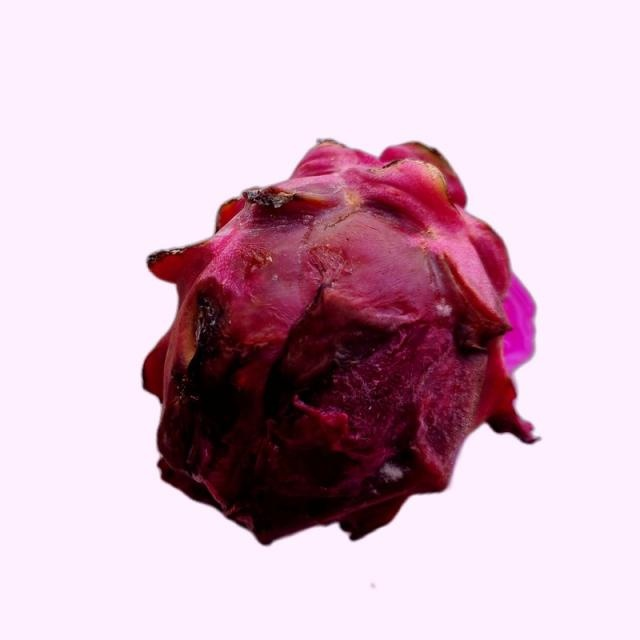
\includegraphics[width=3.05cm]{dragon/start_to_rot/DE02E2-1_JPG.rf.33f73958c3afb2901cca8030862cb986.jpg} &
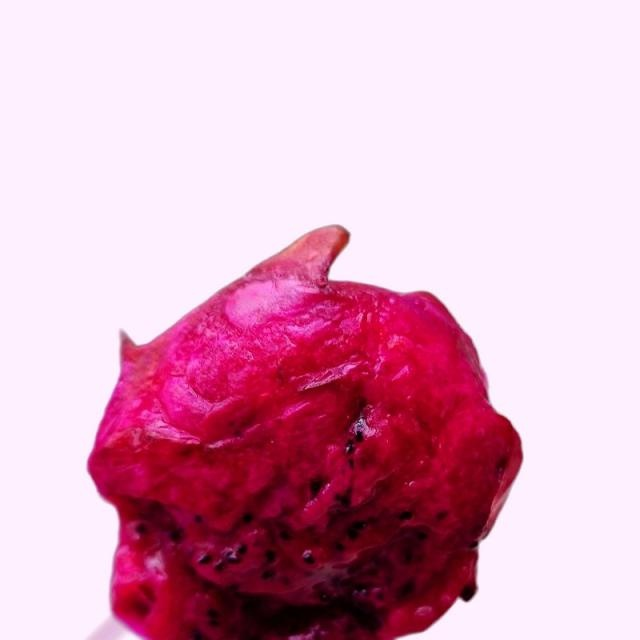
\includegraphics[width=3.05cm]{dragon/start_to_rot/DE1D03-1_JPG.rf.24973ea5aae6ea08f615319006293eeb.jpg} &
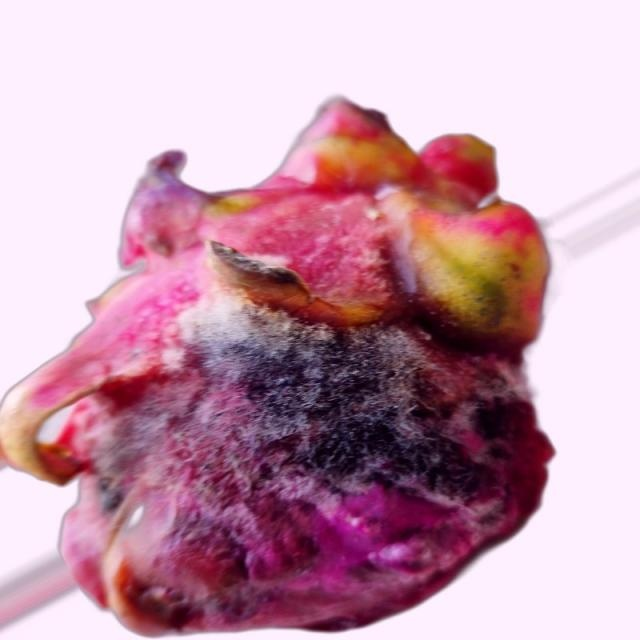
\includegraphics[width=3.05cm]{dragon/start_to_rot/DE1E2A-1_JPG.rf.bea113ab5961f2fc3433f4039ae3d06c.jpg} \\
\cline{2-5}
 & Bad &
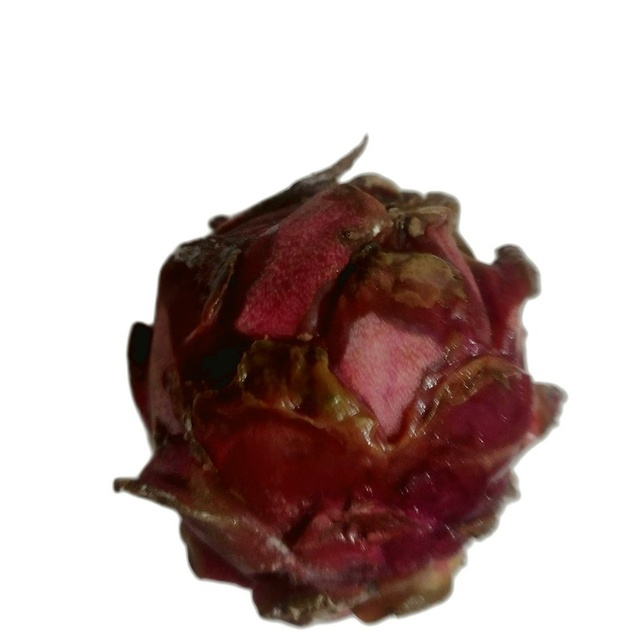
\includegraphics[width=3.05cm]{dragon/bad/Defect_Dragon_Original_Data0011.jpg} &
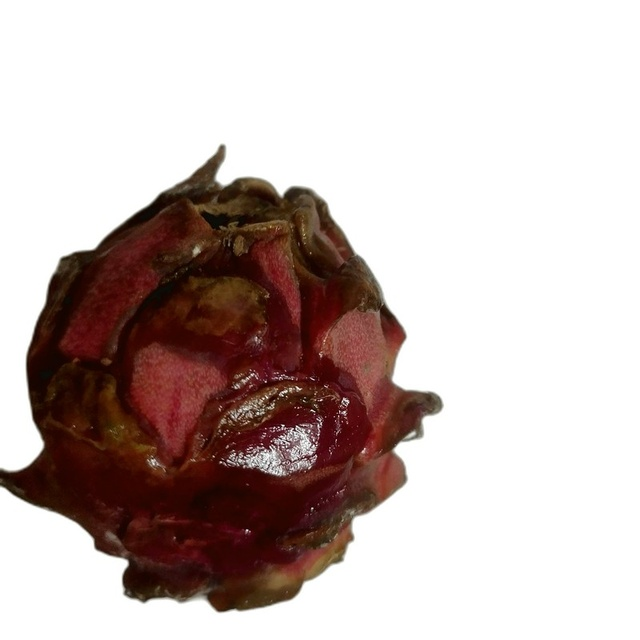
\includegraphics[width=3.05cm]{dragon/bad/Defect_Dragon_Original_Data0012.jpg} &
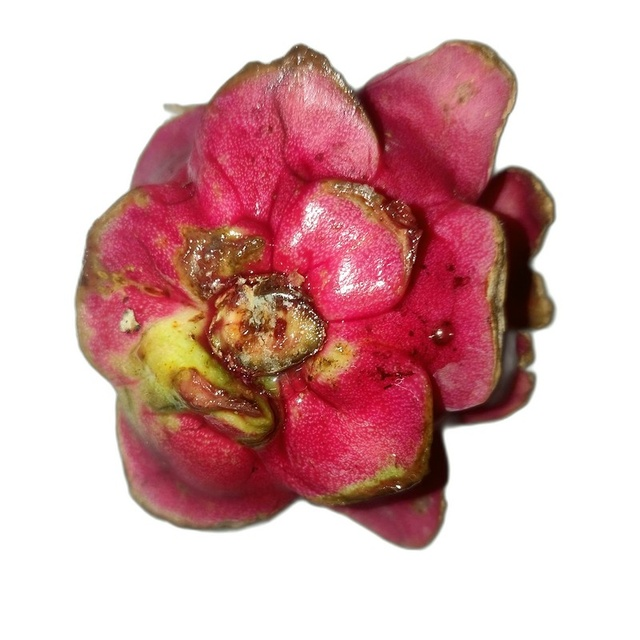
\includegraphics[width=3.05cm]{dragon/bad/Defect_Dragon_Original_Data0047.jpg} \\
\hline

\multirow{3}{*}{Pineapple} & Good &
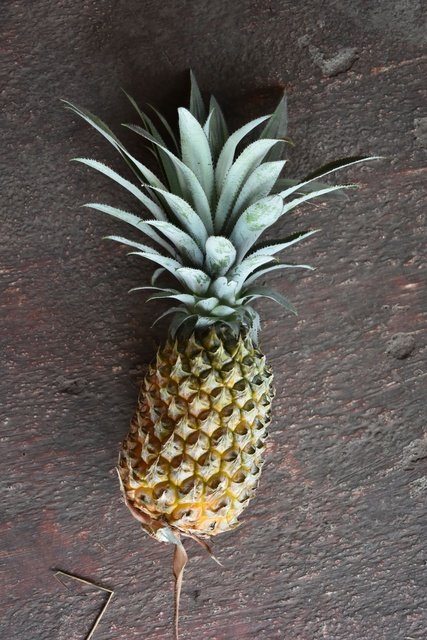
\includegraphics[width=3.05cm]{pineapple/gd3/DSC_5885.jpg} &
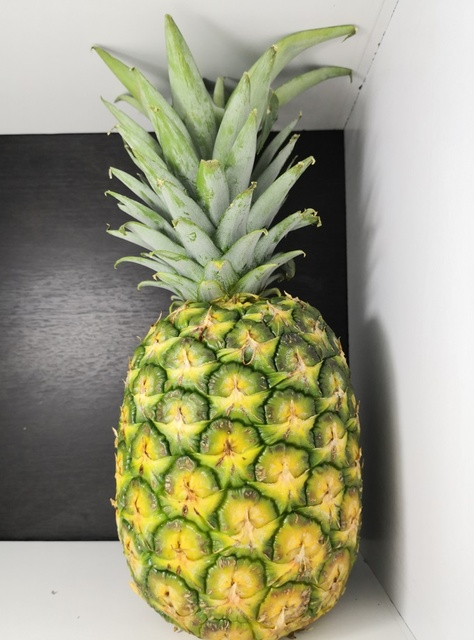
\includegraphics[width=3.05cm]{pineapple/gd3/2_cuatro.jpg} &
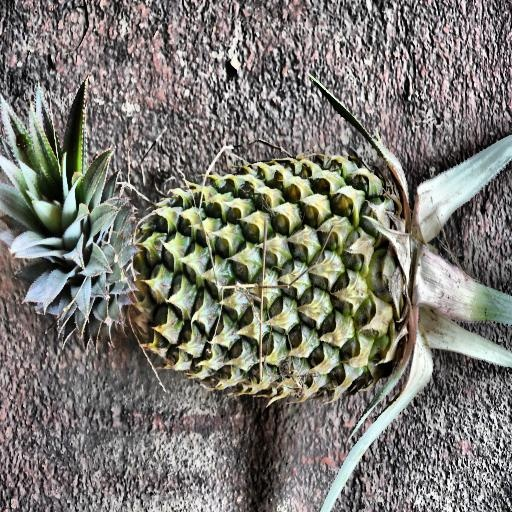
\includegraphics[width=3.05cm]{pineapple/gd3/pineapple_fresh_raw_526_jpg.rf.892852cc9f44a5d5ab154143c6f337b1.jpg} \\
\cline{2-5}
 & Medium &
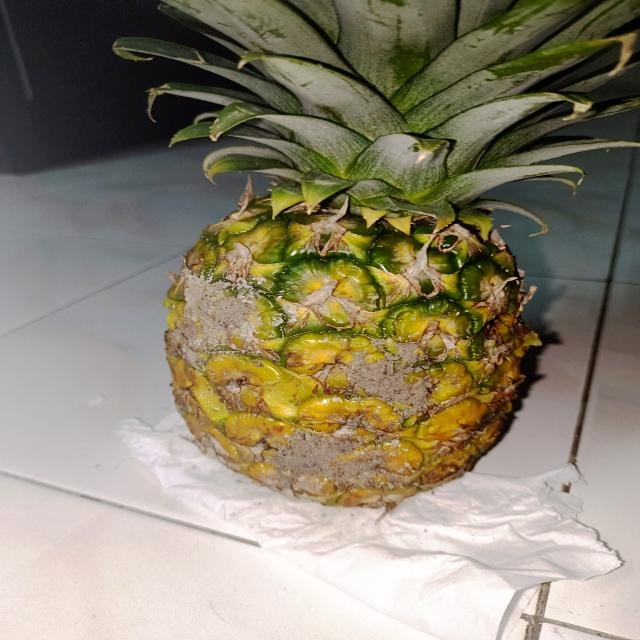
\includegraphics[width=3.05cm]{pineapple/md3/IMG_20230913_195212_jpg.rf.4fb6f792dc782f646fa766b828f744ff.jpg} &
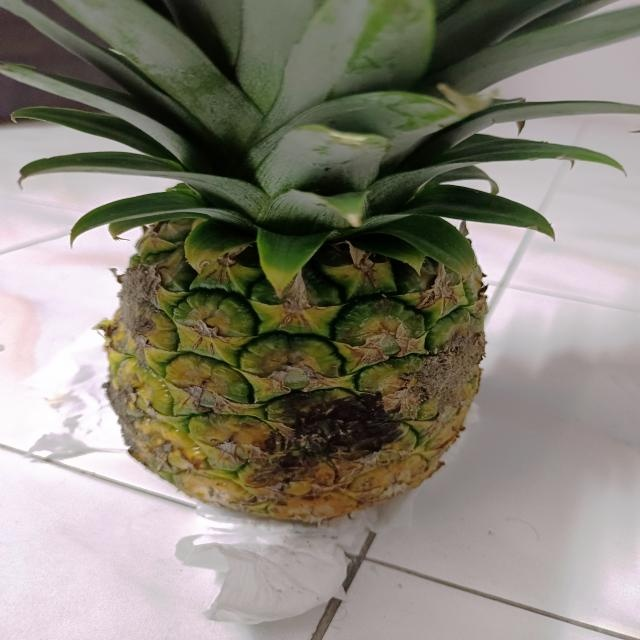
\includegraphics[width=3.05cm]{pineapple/md3/IMG_20230913_195239_jpg.rf.44aed74df6127164f46a73ca9f12824d.jpg} &
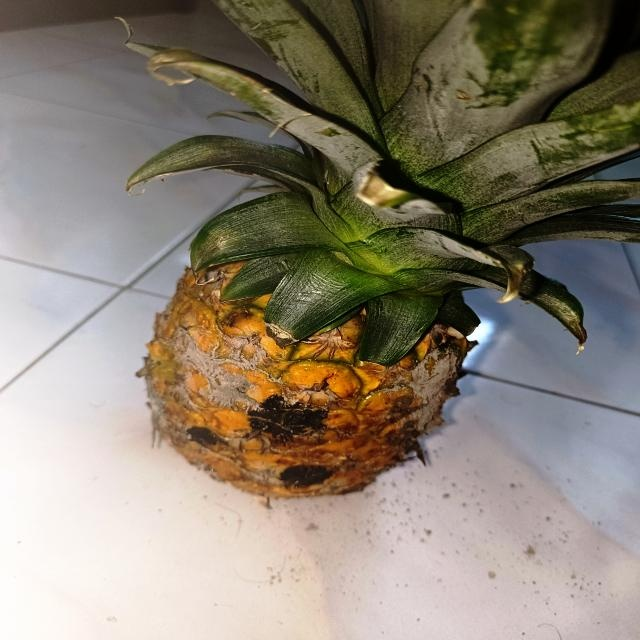
\includegraphics[width=3.05cm]{pineapple/md3/IMG_20230914_161017-1-_jpg.rf.d4993ec954883a3b872f4ca3544fe75a.jpg} \\
\cline{2-5}
 & Bad &
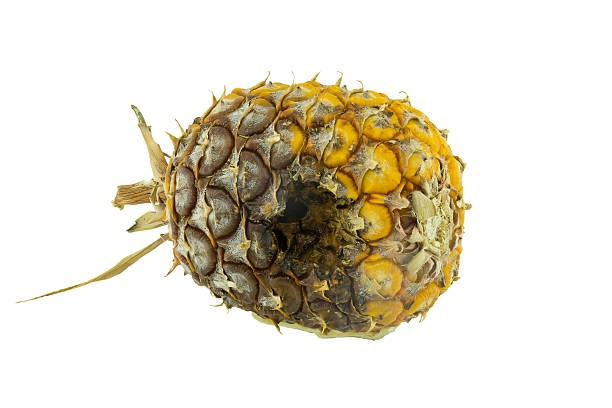
\includegraphics[width=3.05cm]{pineapple/bd3/istockphoto-513935806-612x612.jpg} &
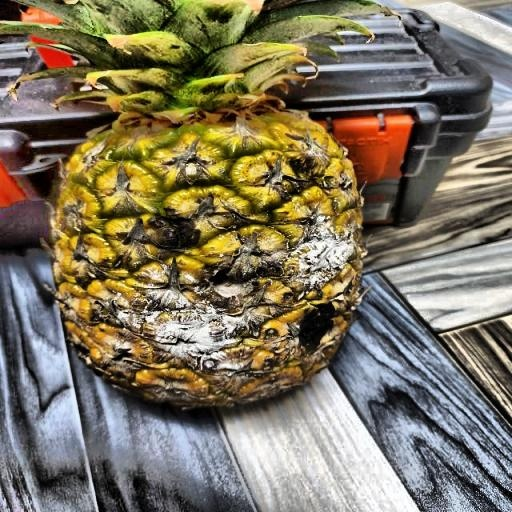
\includegraphics[width=3.05cm]{pineapple/bd3/pineapple_rotten_ripe_3277_jpg.rf.0df2d98f14e94339102f04f8bfd8e1f9.jpg} &
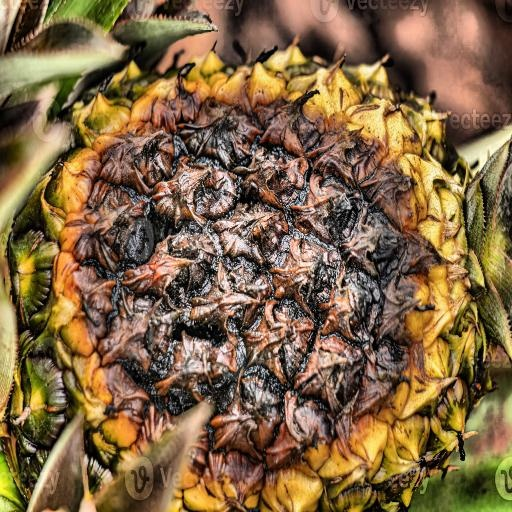
\includegraphics[width=3.05cm]{pineapple/bd3/pineapple-fruit-rotting-on-the-plant-photo_jpg.rf.35b3a38ac9806177bee3252641b1af5b.jpg} \\
\hline

\multirow{3}{*}{Sapodilla} & Good &
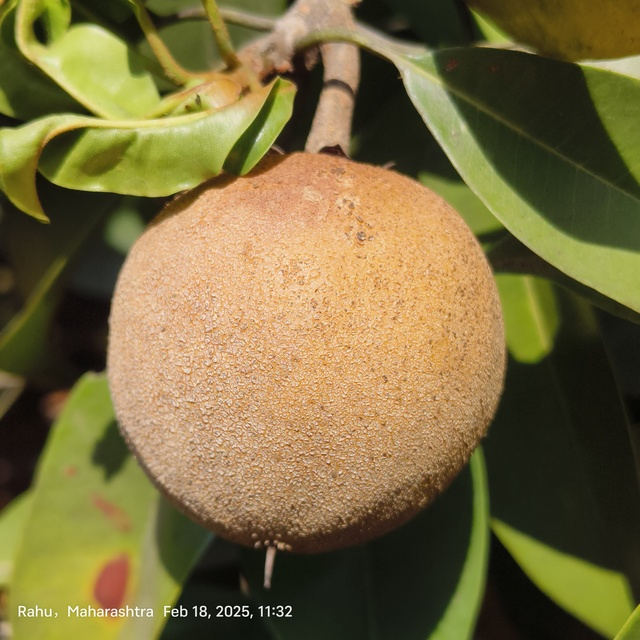
\includegraphics[width=3.05cm]{sofeda/gd3/gd (1).jpg} &
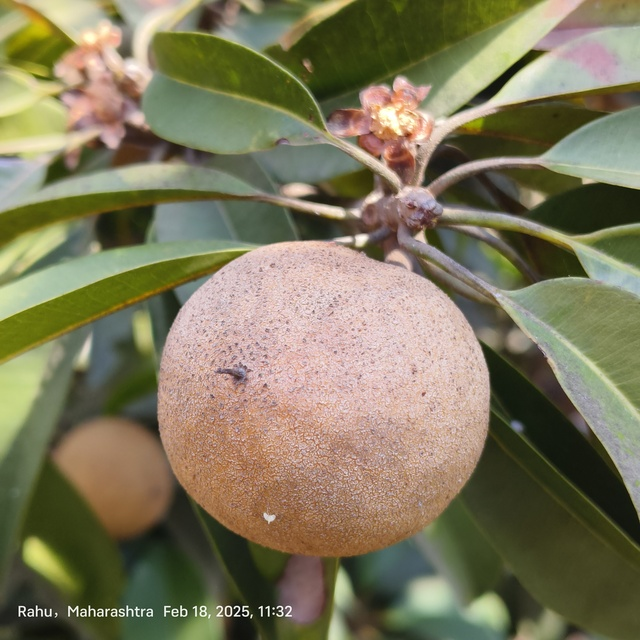
\includegraphics[width=3.05cm]{sofeda/gd3/gd (2).jpg} &
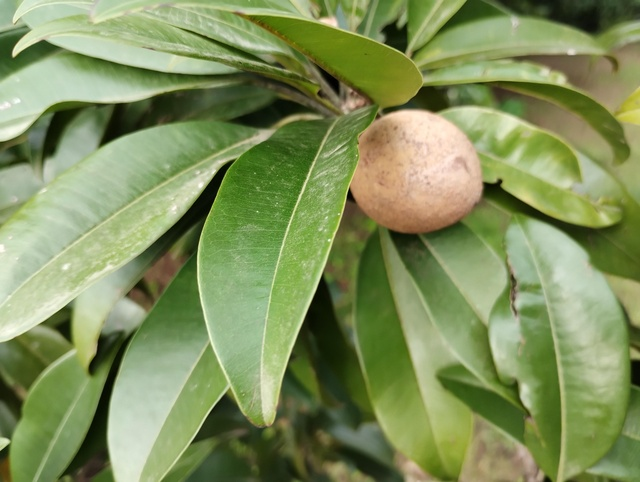
\includegraphics[width=3.05cm]{sofeda/gd3/gd (3).jpg} \\
\cline{2-5}
 & Medium &
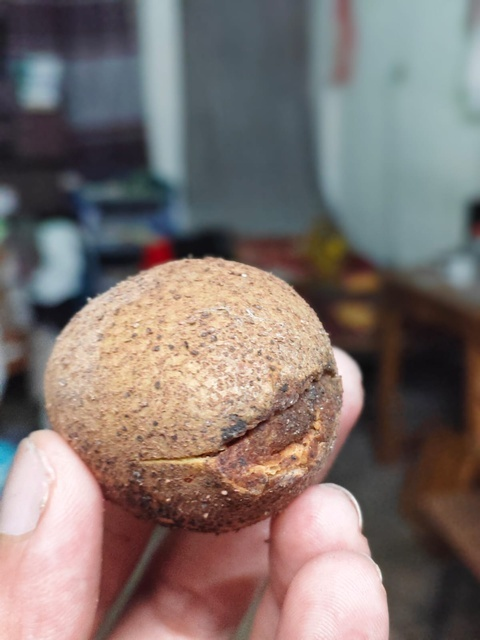
\includegraphics[width=3.05cm]{sofeda/med3/md (1).jpg} &
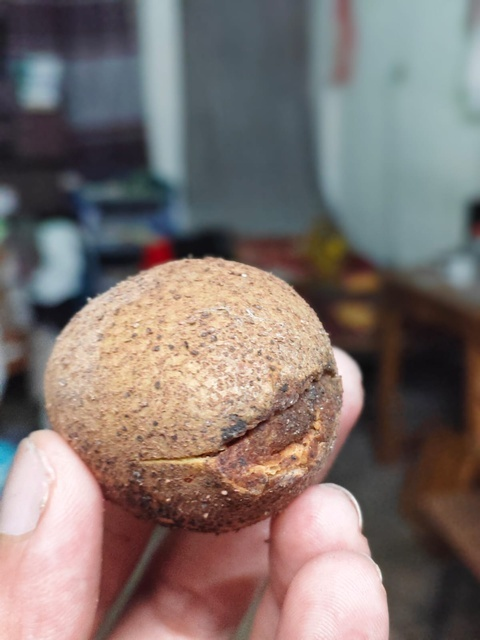
\includegraphics[width=3.05cm]{sofeda/med3/md (1).jpg} &
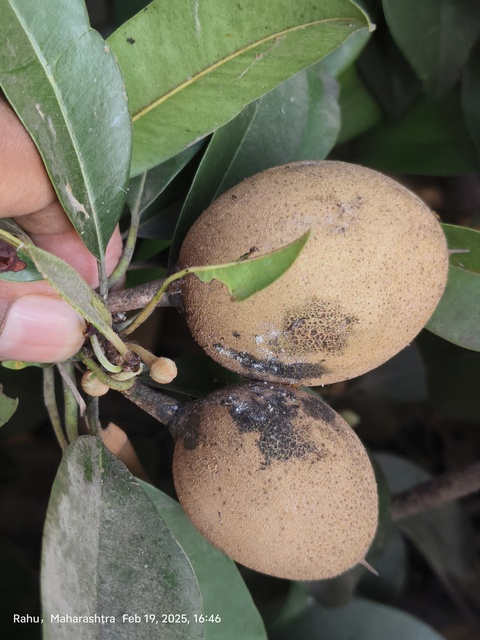
\includegraphics[width=3.05cm]{sofeda/med3/md (2).jpg} \\
\cline{2-5}
 & Bad &
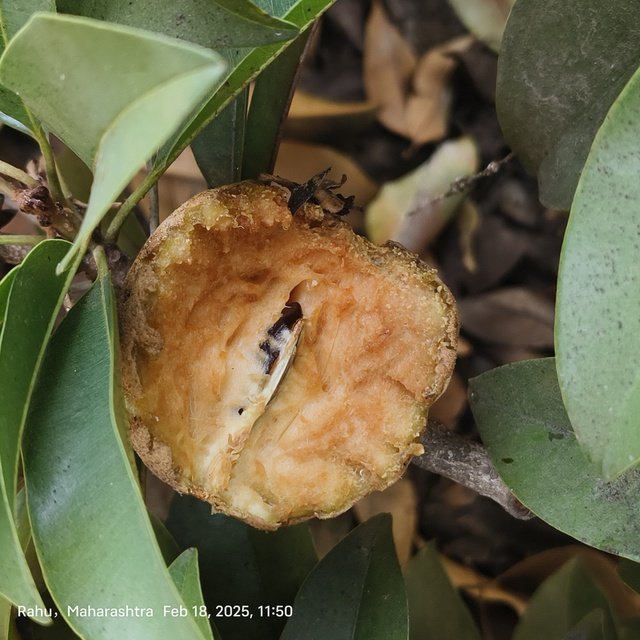
\includegraphics[width=3.05cm]{sofeda/bd3/bd1 (1).jpg}&
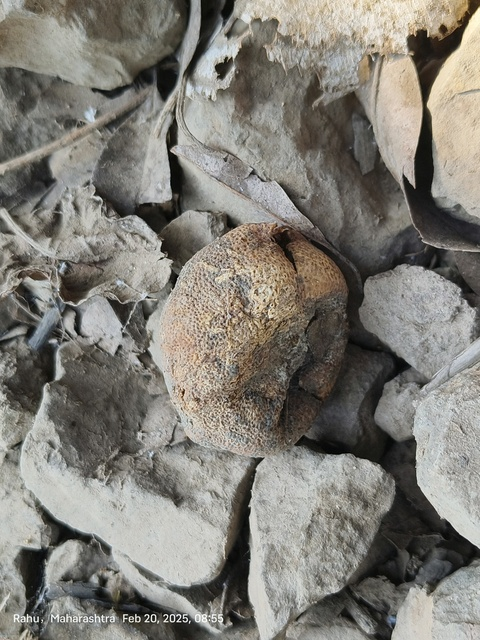
\includegraphics[width=3.05cm]{sofeda/bd3/bd1 (2).jpg} &
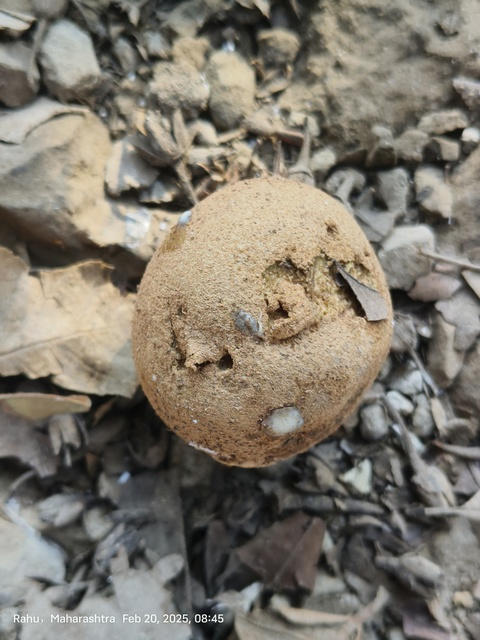
\includegraphics[width=3.05cm]{sofeda/bd3/bd1 (3).jpg} \\
\hline

\multirow{3}{*}{\shortstack{Custard\\apple}} & Good &
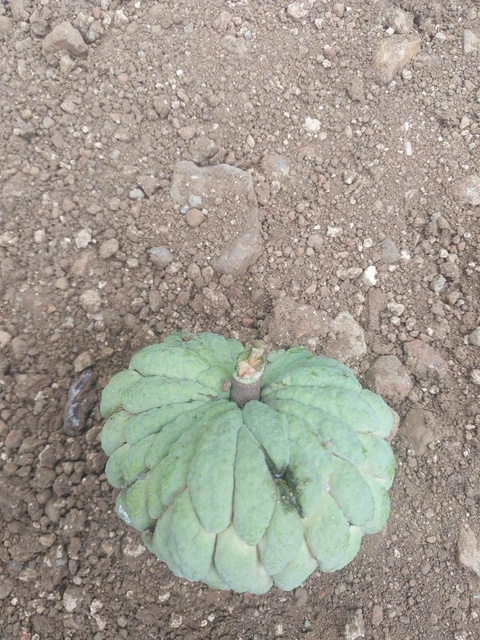
\includegraphics[width=3.05cm]{Custard apple/g1.jpg} &
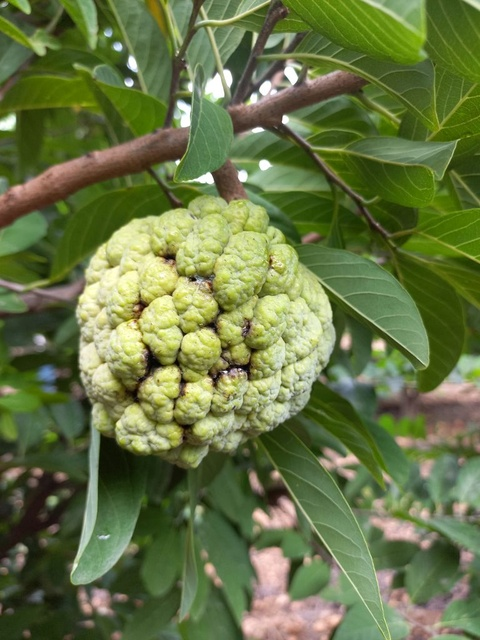
\includegraphics[width=3.05cm]{Custard apple/g2.jpg} &
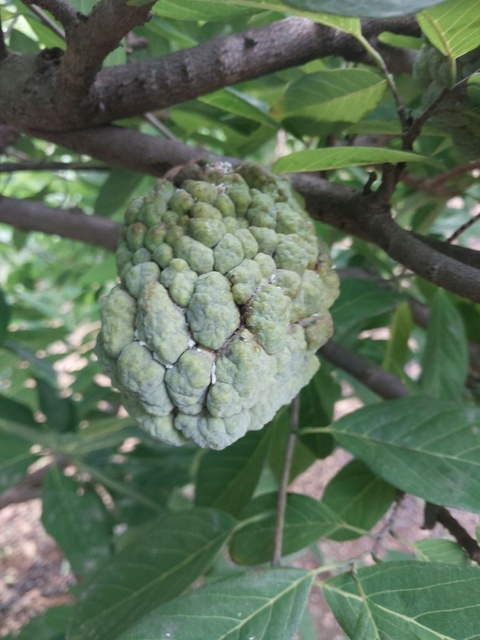
\includegraphics[width=3.05cm]{Custard apple/g3.jpg} \\
\cline{2-5}
 & Medium &
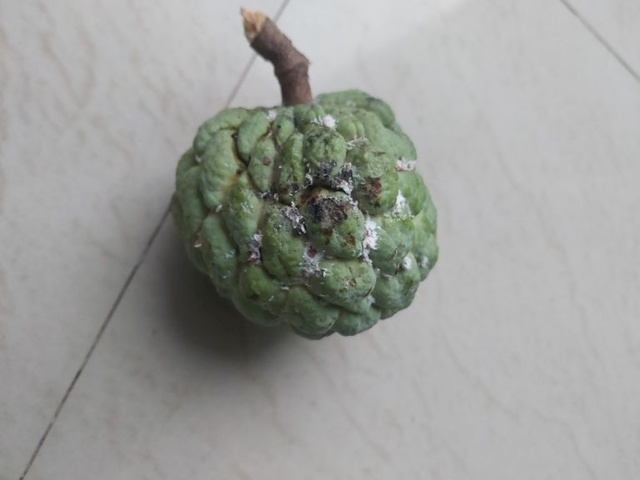
\includegraphics[width=3.05cm]{Custard apple/m1.jpg} &
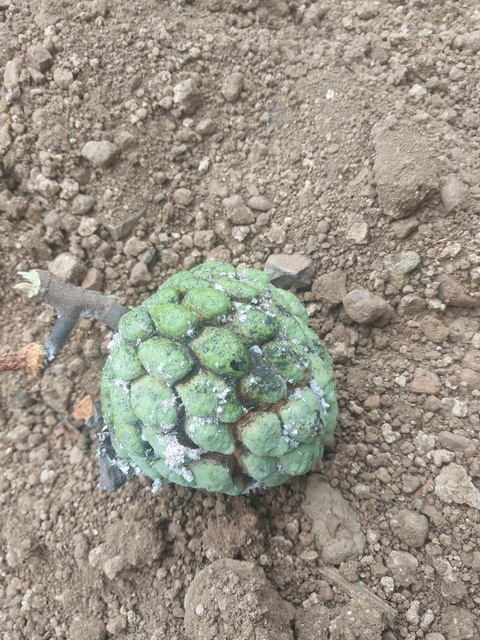
\includegraphics[width=3.05cm]{Custard apple/m2.jpg} &
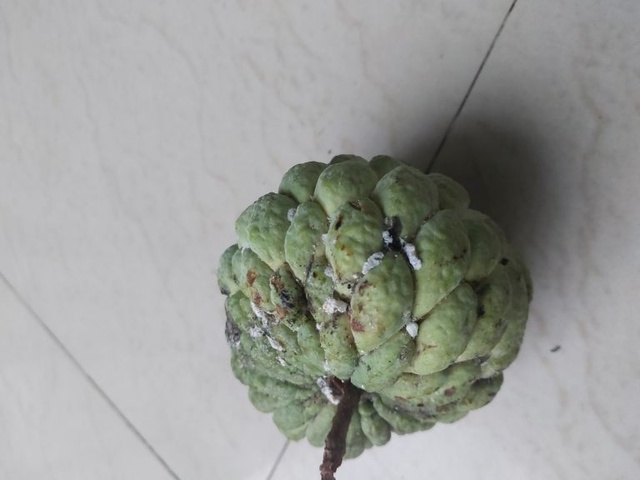
\includegraphics[width=3.05cm]{Custard apple/m3.jpg} \\
\cline{2-5}
 & Bad &
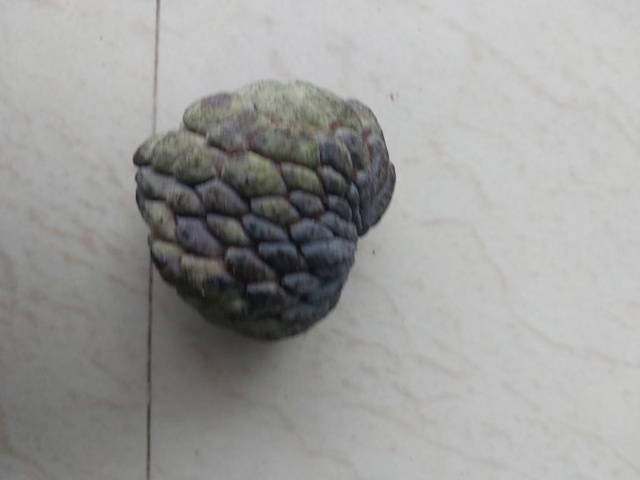
\includegraphics[width=3.05cm]{Custard apple/b1.jpg} &
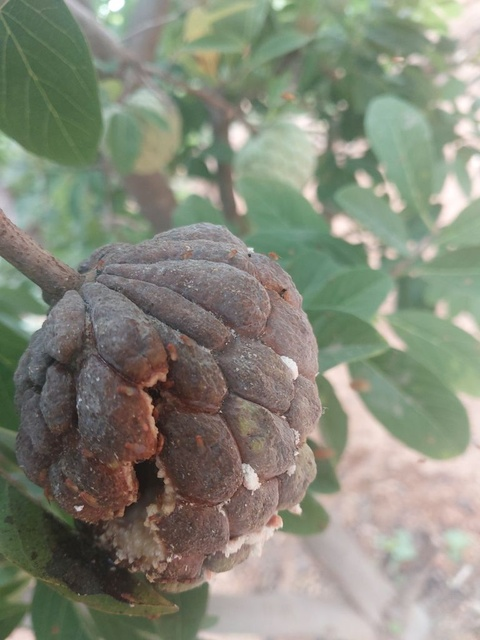
\includegraphics[width=3.05cm]{Custard apple/b2.jpg} &
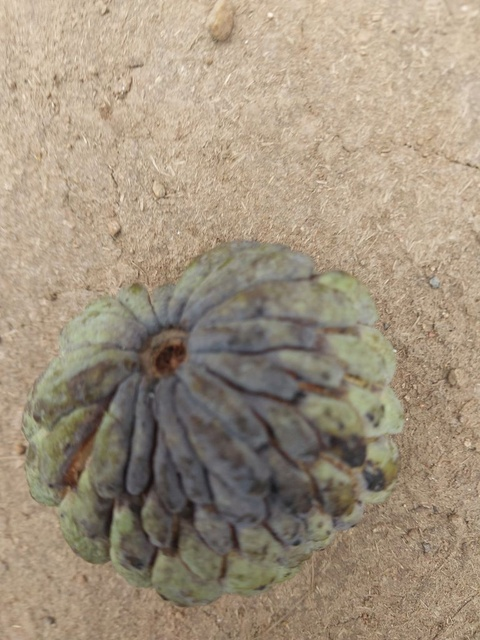
\includegraphics[width=3.05cm]{Custard apple/b3.jpg} \\
\hline

\end{longtable}


% =========================================================
% 8. DATA PREPROCESSING, CURATION AND LEAKAGE CONTROL
% =========================================================
\section{Data Preprocessing, Curation and Leakage Control}
Transformations from raw images to the released machine-learning-ready datasets followed strict pipeline isolation to prevent data leakage.

\begin{itemize}
    \item \textbf{Data Cleaning:} Duplicate and near-duplicate images were identified and removed using perceptual hashing (pHash) with a Hamming distance threshold $\le 4$. Corrupt files and images with non-standard EXIF rotations were normalized.
    \item \textbf{Missing Data Handling:} Corrupted or unreadable image headers were discarded during the ingestion audit. Missing labels were not permitted; every retained image possesses verified species and grade tags.
    \item \textbf{Outliers and Noise Filtering:} Extremely blurry captures (Laplacian variance $< 100$) and images where the fruit covered less than 20\% of the bounding area were purged.
    \item \textbf{Resizing and Scaling:} All images were bilinearly interpolated and standardized to $224 \times 224$ pixels, matching standard deep neural network input requirements while preserving aspect ratios via center cropping.
    \item \textbf{Normalization:} Pixel intensities were normalized to $[0, 1]$ and subsequently standardized using ImageNet RGB channel means ($\mu = [0.485, 0.456, 0.406]$) and standard deviations ($\sigma = [0.229, 0.224, 0.225]$).
    \item \textbf{Contrast Enhancement (CLAHE):} Contrast Limited Adaptive Histogram Equalization was applied to equalize illumination across shadows and highlight subtle localized peel abrasions.
    \item \textbf{Data Augmentation:} Augmentations were applied exclusively to training splits: random rotations ($\pm 30^\circ$), horizontal and vertical flips, random scaling/zooming ($0.8 \times$ to $1.2 \times$), and brightness/contrast jitter ($\pm 15\%$).
    \item \textbf{Strict Leakage Control:} Data partitioning was executed on the original, unique image set \emph{prior} to any augmentation. Test partitions contain solely raw, unaugmented photographic captures, ensuring zero cross-split leakage.
\end{itemize}

\subsection{Resizing / Scaling}
All images are resized to a fixed input resolution of $224 \times 224$ pixels so that they match the standardized input shape required by the CNN and transfer-learning architectures.

\begin{figure}[H]
    \centering
    \begin{subfigure}[b]{0.35\textwidth}
        \centering
        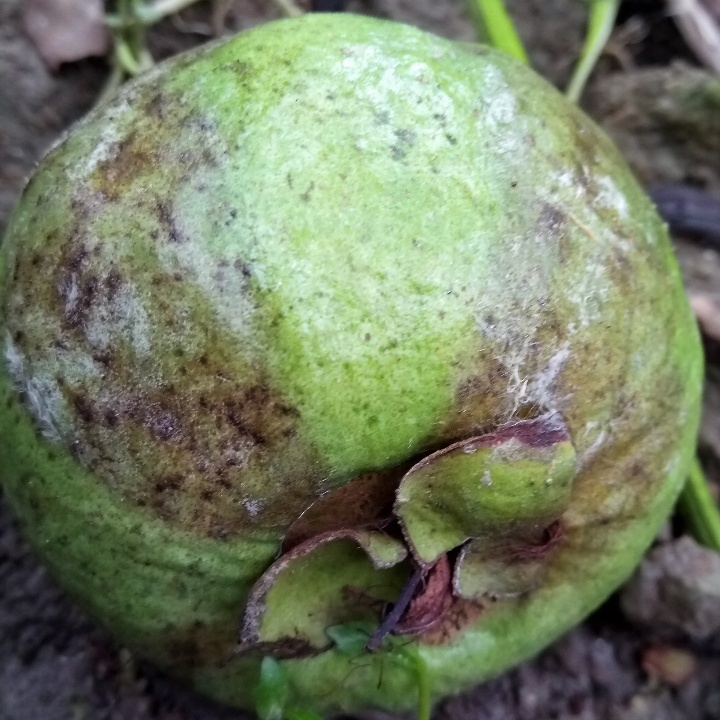
\includegraphics[width=\textwidth]{augment/original.jpg}
        \caption{Original input image}
    \end{subfigure}
    \hspace{1cm}
    \begin{subfigure}[b]{0.35\textwidth}
        \centering
        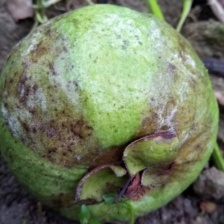
\includegraphics[width=\textwidth]{augment/resized_224x224.jpg}
        \caption{Resized image ($224\times224$)}
    \end{subfigure}
    \caption{Example of image resizing and scaling}
    \label{fig:resize-example}
\end{figure}

\subsection{Normalization}
Pixel intensity values (originally in the range $[0, 255]$) are rescaled to $[0, 1]$ or standardized using the dataset channel mean $\mu$ and standard deviation $\sigma$:

\begin{equation}
    x_{norm} = \frac{x - \mu}{\sigma}
\end{equation}

Normalization stabilizes gradient descent updates, accelerates model convergence, and ensures balanced weight learning across color channels.

\subsection{Contrast Adjustment (CLAHE)}
Contrast Limited Adaptive Histogram Equalization (CLAHE) is applied to enhance local contrast without over-amplifying noise. This highlights subtle surface defects, blemishes, and texture variations crucial for differentiating quality grades.

\begin{figure}[H]
    \centering
    \begin{subfigure}[b]{0.38\textwidth}
        \centering
        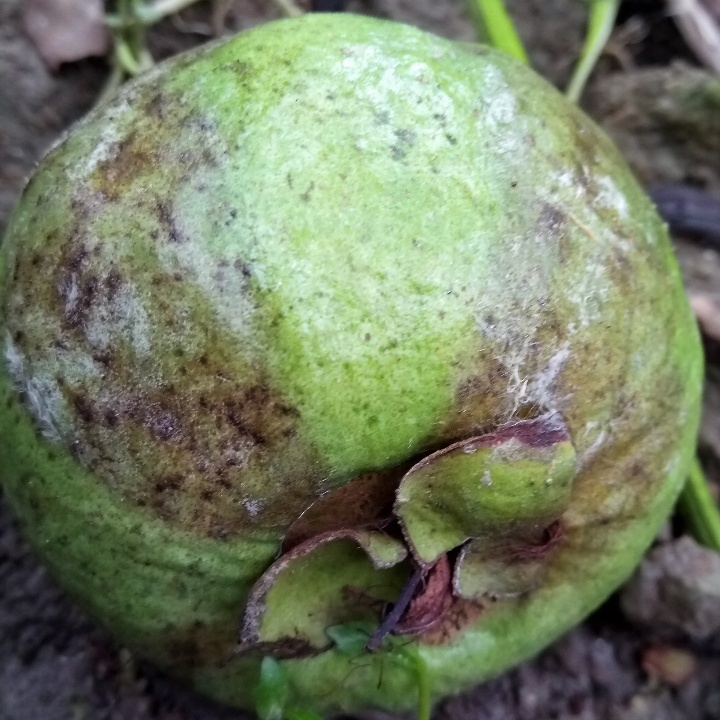
\includegraphics[width=\textwidth]{augment/original.jpg}
        \caption{Original image}
    \end{subfigure}
    \hspace{1cm}
    \begin{subfigure}[b]{0.38\textwidth}
        \centering
        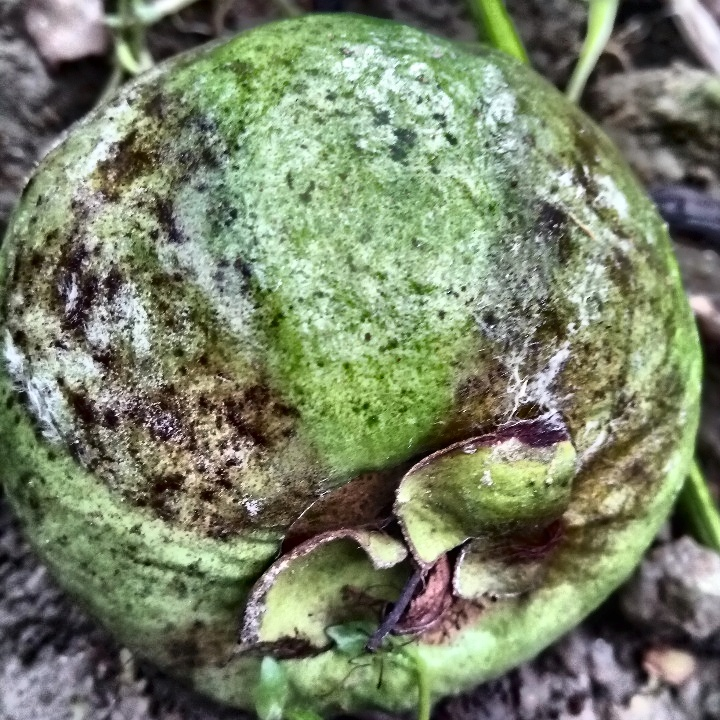
\includegraphics[width=\textwidth]{augment/clahe_enhanced.jpg}
        \caption{CLAHE contrast enhanced}
    \end{subfigure}
    \caption{Example of CLAHE contrast enhancement}
    \label{fig:contrast-example}
\end{figure}

\subsection{Data Augmentation}
To artificially increase dataset diversity, simulate varied lighting/environmental conditions, and prevent model overfitting, multiple augmentation techniques are applied during training:
\begin{itemize}
    \item \textbf{Rotation} ($\pm 30^\circ$)
    \item \textbf{Horizontal / Vertical Flip}
    \item \textbf{Random Zoom / Cropping}
    \item \textbf{Brightness Variation}
\end{itemize}

\begin{figure}[H]
    \centering
    \begin{subfigure}[b]{0.18\textwidth}
        \centering
        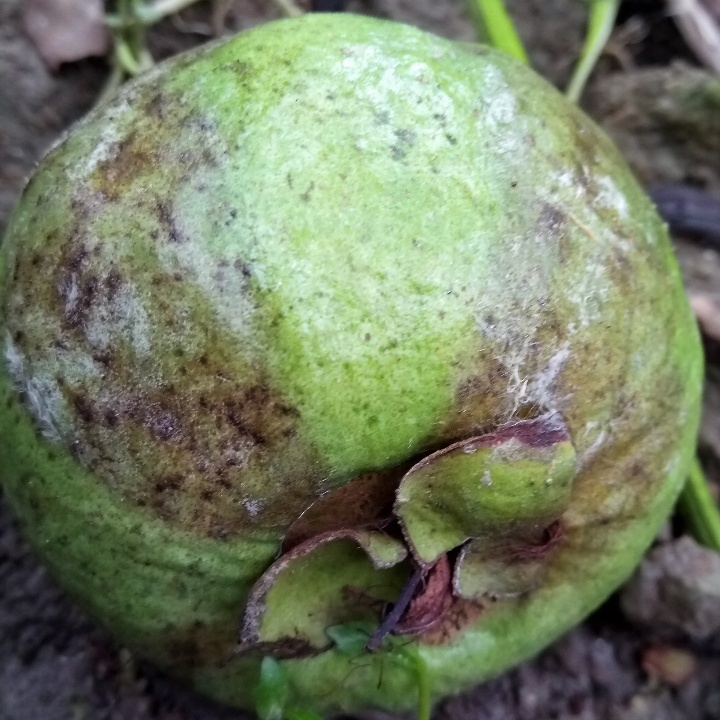
\includegraphics[width=\textwidth]{augment/original.jpg}
        \caption{Original}
    \end{subfigure}
    \hfill
    \begin{subfigure}[b]{0.18\textwidth}
        \centering
        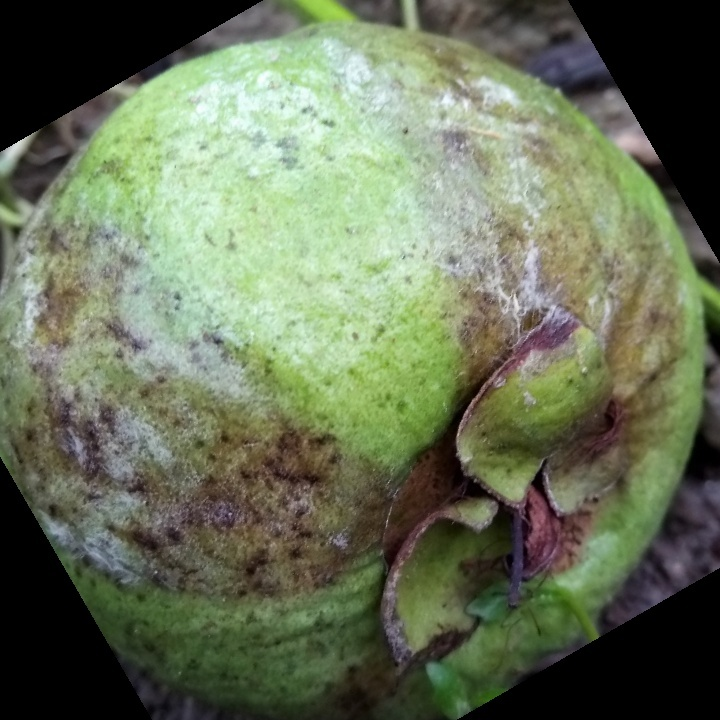
\includegraphics[width=\textwidth]{augment/rotated.jpg}
        \caption{Rotated}
    \end{subfigure}
    \hfill
    \begin{subfigure}[b]{0.18\textwidth}
        \centering
        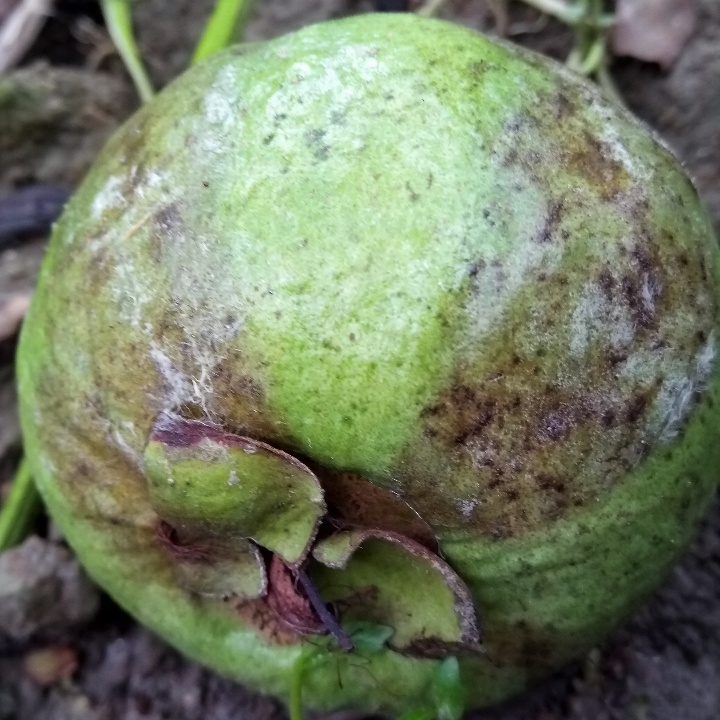
\includegraphics[width=\textwidth]{augment/flipped.jpg}
        \caption{Flipped}
    \end{subfigure}
    \hfill
    \begin{subfigure}[b]{0.18\textwidth}
        \centering
        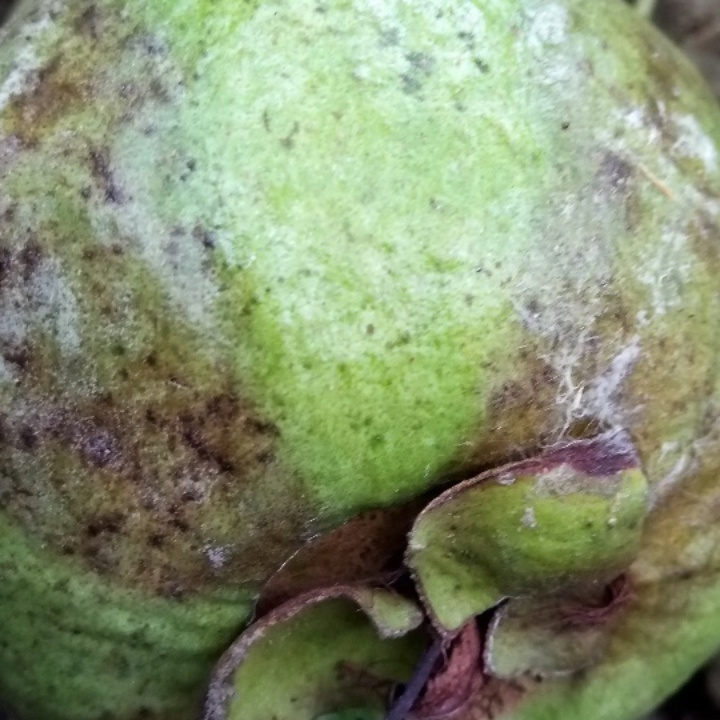
\includegraphics[width=\textwidth]{augment/zoomed.jpg}
        \caption{Zoomed}
    \end{subfigure}
    \hfill
    \begin{subfigure}[b]{0.18\textwidth}
        \centering
        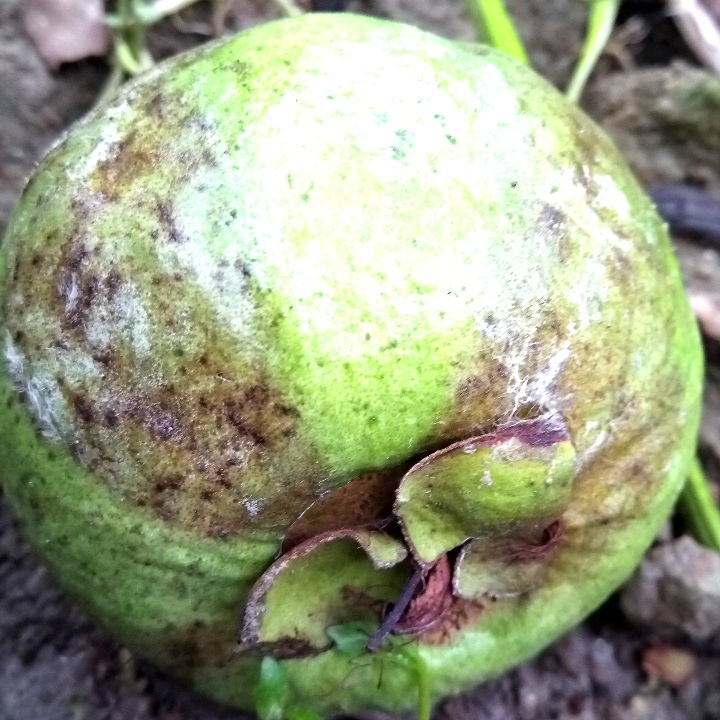
\includegraphics[width=\textwidth]{augment/brightness.jpg}
        \caption{Brightness}
    \end{subfigure}
    \caption{Data augmentation transformations applied to a sample image}
    \label{fig:augmentation-example}
\end{figure}


% =========================================================
% 9. TECHNICAL VALIDATION AND DATA QUALITY
% =========================================================
\section{Technical Validation and Data Quality}
The integrity of the dataset was verified along seven distinct quality dimensions prior to baseline benchmarking, as summarized in Table~\ref{tab:data-quality-checks}.

\begin{table}[H]
\centering\small
\begin{tabular}{@{}p{0.25\textwidth}p{0.71\textwidth}@{}}
\toprule
\textbf{Quality Dimension} & \textbf{Evidence and Checks Performed} \\
\midrule
\textbf{Completeness} & All 20,823 images possess validated labels and verified RGB channels. No missing or null values exist in the dataset manifest. \\
\midrule
\textbf{Consistency} & All released images are strictly formatted to 24-bit RGB JPEG/PNG format, scaled uniformly to $224 \times 224$ pixels with standardized lowercase directory paths. \\
\midrule
\textbf{Label Quality} & Two-tier verification: initial classification by designated team member followed by cross-review by a secondary member. Borderline cases adjudicated jointly. \\
\midrule
\textbf{Measurement Quality} & Optical clarity confirmed via Laplacian blur variance thresholding ($> 100$). Standardized color balance verified under varied indoor and field illumination. \\
\midrule
\textbf{Integrity} & Cryptographic SHA-256 checksums computed for every file to verify corruption-free archival and reproducible download verification. \\
\midrule
\textbf{Representativeness} & Balanced representation across 13 diverse fruits with balanced quality distributions ($\approx 500$--$600$ images per quality class per fruit). \\
\midrule
\textbf{Reproducibility} & Fully deterministic data processing pipeline with explicit random seeds (seed 42) and standalone Python scripts. \\
\bottomrule
\end{tabular}
\caption{Data quality validation dimensions and verification evidence}
\label{tab:data-quality-checks}
\end{table}

\subsection{Comparison with Existing Datasets and Significance}
Table~\ref{tab:comparison-existing-datasets} contrasts the proposed dataset against well-known public benchmarks in the fruit classification literature.

\begin{table}[H]
\centering\small
\begin{tabularx}{\textwidth}{@{}p{0.20\textwidth}cccp{0.16\textwidth}X@{}}
\toprule
\textbf{Dataset} & \textbf{Total Images} & \textbf{Fruits} & \textbf{Quality Grades} & \textbf{Background} & \textbf{Key Distinctions} \\
\midrule
Fruit-360 \cite{fruit360} & 90,483 & 131 & None (Only Type) & White / Studio & Studio rotary setup; no defect or quality grading. \\
FruitNet (Indian) \cite{fruitnet} & 14,700 & 6 & 2 (Good / Bad) & Complex & Binary condition only; limited to 6 fruit types. \\
Fresh/Rotten \cite{khalil_fresh_rotten} & 13,599 & 3 & 2 (Fresh / Rotten) & Mixed & Only 3 fruits (Apple, Banana, Orange); binary only. \\
\textbf{Our Dataset} & \textbf{20,823} & \textbf{13} & \textbf{3 (Good/Med/Bad)} & \textbf{Real-World} & \textbf{13 fruits, 3-tier grading (with Medium), multi-source.} \\
\bottomrule
\end{tabularx}
\caption{Comparison with existing public fruit classification datasets}
\label{tab:comparison-existing-datasets}
\end{table}

The dataset introduces several novel properties:
\begin{enumerate}
    \item \textbf{Comprehensive 13-Fruit Regional Breadth:} Encompasses major tropical and domestic species—including under-represented cultivars like Sapodilla, Custard Apple, Jujube, Star Fruit, and Jackfruit—seldom represented in mainstream benchmarks.
    \item \textbf{Granular 3-Tier Quality Annotation:} Introduces an explicit \texttt{medium} grade capturing initial blemishes and partial ripeness, reflecting operational post-harvest supply chain realities.
    \item \textbf{Ecological Background Variety:} Incorporates realistic shadows, natural foliage, wooden market crates, and packaging trays, preparing models for robust on-field and conveyor deployment.
\end{enumerate}

% =========================================================
% 10. MACHINE LEARNING (ML) USE DEMONSTRATION
% =========================================================
\section{Machine Learning (ML) Use Demonstration}
The primary objective is to prove the dataset's validity and usability in supporting machine learning workflows.

\subsection{ML Task Definition}
We establish two distinct supervised learning tasks:
\begin{itemize}
    \item \textbf{Task 1 (Macro Fruit-Type Recognition):} Given an RGB image $X \in \mathbb{R}^{224 \times 224 \times 3}$, predict the fruit species label $y \in \{1, 2, \dots, 13\}$ across all 20,823 images.
    \item \textbf{Task 2 (Intra-Class Quality Classification):} For each of the 13 fruit varieties independently, predict the quality condition $y \in \{\text{Good}, \text{Medium}, \text{Bad}\}$ from a single input image.
\end{itemize}

\subsection{Data Partitioning Strategy}
Each dataset was split into 80\% training and 20\% test sets using stratified random sampling with a fixed random seed (\texttt{seed = 42}). Stratification guarantees identical class proportions across both splits. Augmentation was strictly applied solely during training epochs.

\subsection{Preprocessing and Representation Steps}
Images were resized to $224 \times 224$, CLAHE-enhanced, normalized to ImageNet statistics, and converted to PyTorch tensors. All feature extractors operated on these standardized representations.

\subsection{ML Models and Hyperparameters}
Five candidate architectures were benchmarked across the dataset tasks: a lightweight from-scratch Custom CNN baseline and four transfer-learning backbones (MobileNetV3-Large, YOLO26n-cls, EfficientNet-B0, and ResNet-50).

\subsubsection{Custom CNN Architectures}
Two dedicated from-scratch convolutional neural network baselines were developed and benchmarked: a 4-stage architecture for Task~1 (13-Class Macro Fruit Species Classification) and a 3-stage architecture for Task~2 (3-Tier Intra-Fruit Quality Inspection). Figure~\ref{fig:custom-cnn-architectures} illustrates the visual layer block diagrams, while Table~\ref{tab:custom-cnn-13class} and Table~\ref{tab:custom-cnn-quality} outline the sequential layer-by-layer specifications.

\begin{figure}[H]
    \centering
    \begin{subfigure}[b]{\textwidth}
        \centering
        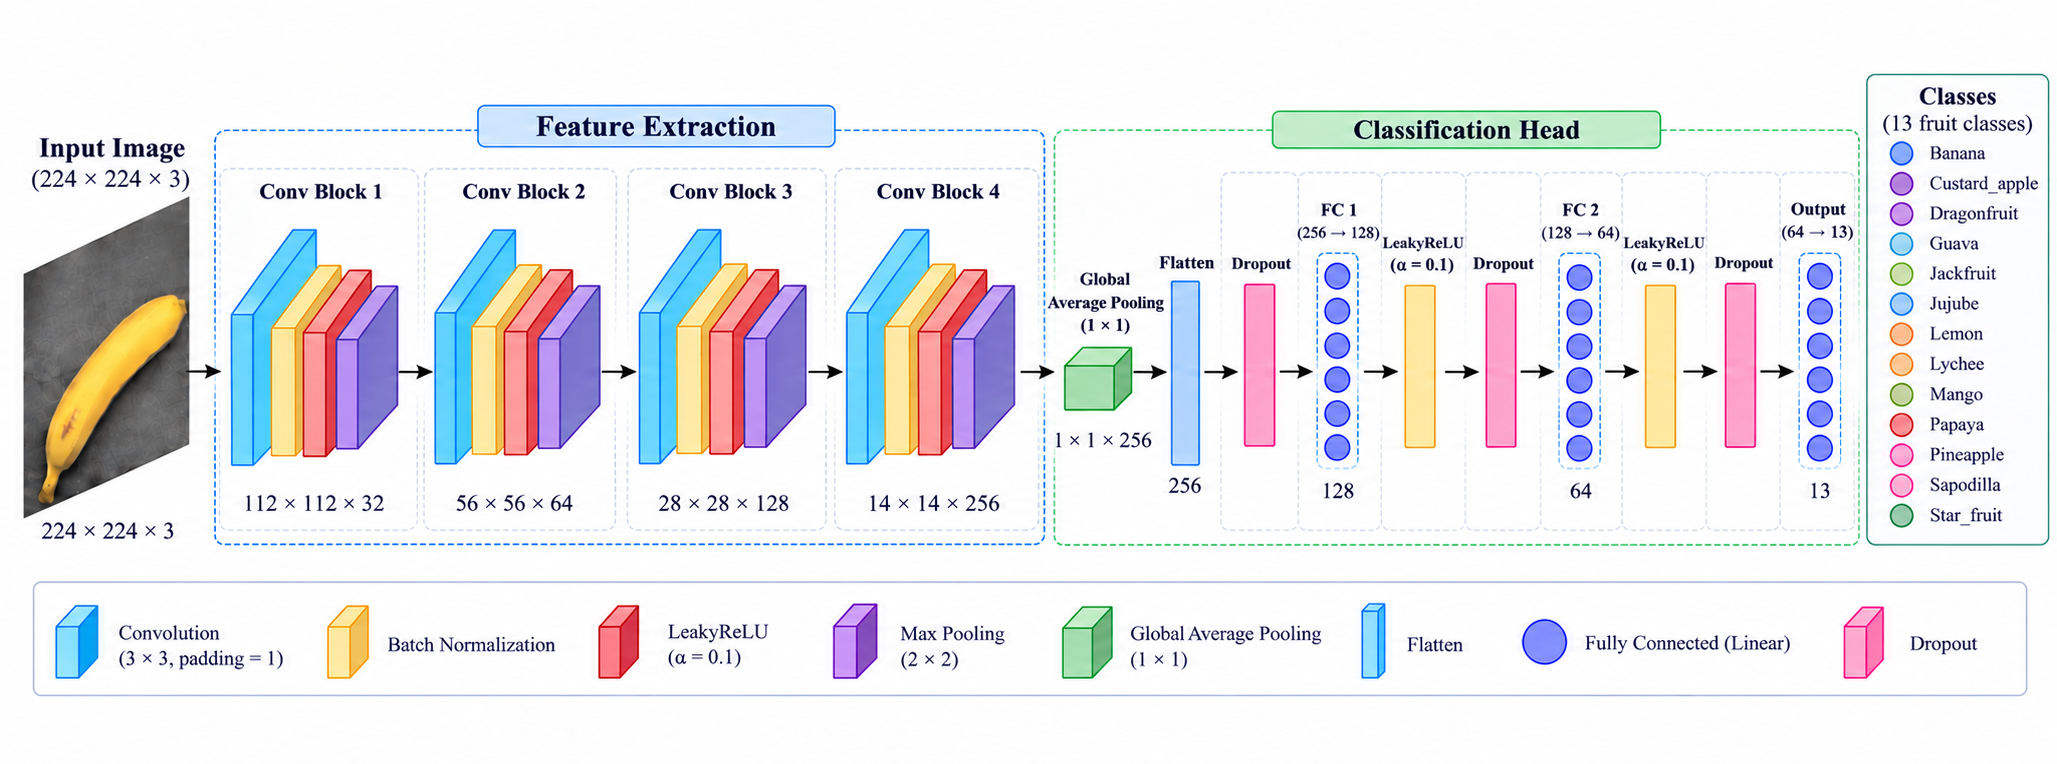
\includegraphics[width=\textwidth]{cnn1.png}
        \caption{Custom CNN architecture diagram (Task 1: 13-Class Multi-Fruit Species Recognition)}
        \label{fig:custom-cnn-13class}
    \end{subfigure}
    \vspace{0.3cm}
    \begin{subfigure}[b]{\textwidth}
        \centering
        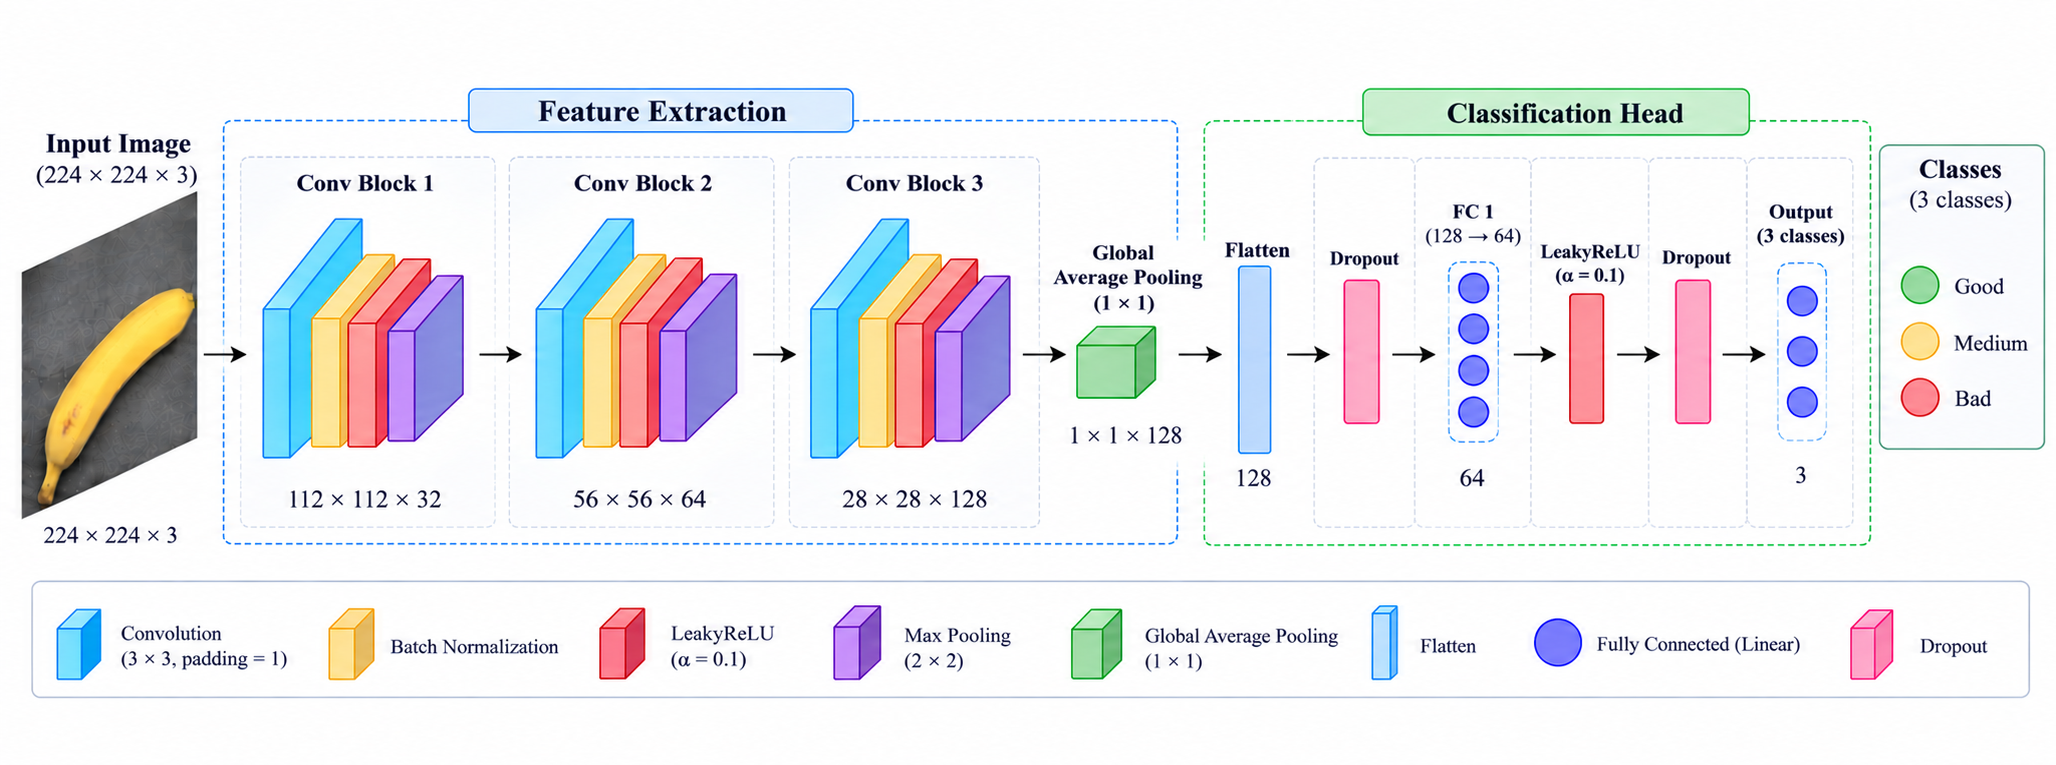
\includegraphics[width=\textwidth]{cnn2.png}
        \caption{Custom CNN architecture diagram (Task 2: 3-Class Intra-Fruit Quality Inspection)}
        \label{fig:custom-cnn-quality}
    \end{subfigure}
    \caption{Layer-by-layer architectural diagrams of the custom convolutional neural network baseline models}
    \label{fig:custom-cnn-architectures}
\end{figure}

\begin{table}[H]
\centering\small
\begin{tabularx}{\textwidth}{@{}l l l X@{}}
\toprule
\textbf{Layer / Stage} & \textbf{Output Shape} & \textbf{Kernel / Config} & \textbf{Operations and Hyperparameters} \\
\midrule
Input Layer & $224 \times 224 \times 3$ & -- & Standardized RGB photographic input \\
\midrule
\multicolumn{4}{@{}l}{\textbf{Feature Extraction Backbone (4 Convolutional Blocks)}} \\
\midrule
Conv Block 1 & $112 \times 112 \times 32$ & $3 \times 3$, pad 1 & Conv2D (32 filters) $\to$ BatchNorm2d $\to$ LeakyReLU($\alpha=0.1$) $\to$ MaxPool2d($2\times2$) \\
Conv Block 2 & $56 \times 56 \times 64$ & $3 \times 3$, pad 1 & Conv2D (64 filters) $\to$ BatchNorm2d $\to$ LeakyReLU($\alpha=0.1$) $\to$ MaxPool2d($2\times2$) \\
Conv Block 3 & $28 \times 28 \times 128$ & $3 \times 3$, pad 1 & Conv2D (128 filters) $\to$ BatchNorm2d $\to$ LeakyReLU($\alpha=0.1$) $\to$ MaxPool2d($2\times2$) \\
Conv Block 4 & $14 \times 14 \times 256$ & $3 \times 3$, pad 1 & Conv2D (256 filters) $\to$ BatchNorm2d $\to$ LeakyReLU($\alpha=0.1$) $\to$ MaxPool2d($2\times2$) \\
\midrule
Global Pooling & $1 \times 1 \times 256$ & -- & AdaptiveAvgPool2d($1 \times 1$) spatial reduction \\
\midrule
\multicolumn{4}{@{}l}{\textbf{Sequential Classification Head ($256 \to 128 \to 64 \to 13$)}} \\
\midrule
Flatten & 256 & -- & Flatten 3D spatial tensor into 1D feature vector \\
Dropout 1 & 256 & $p = 0.3$ & Regularization to prevent neuron co-adaptation \\
Dense Layer 1 & 128 & Linear($256 \to 128$) & Fully-connected feature projection \\
Activation 1 & 128 & LeakyReLU($\alpha=0.1$) & Non-linear activation preventing dying gradients \\
Dropout 2 & 128 & $p = 0.3$ & Intermediate dense layer dropout \\
Dense Layer 2 & 64 & Linear($128 \to 64$) & Bottleneck dense representation \\
Activation 2 & 64 & LeakyReLU($\alpha=0.1$) & Non-linear activation \\
Dropout 3 & 64 & $p = 0.3$ & Pre-output dropout regularization \\
Output Layer & 13 & Linear($64 \to 13$) & Final unnormalized class logits for 13 fruit species \\
\bottomrule
\end{tabularx}
\caption{Custom CNN architecture specification for Task 1: 13-Class Multi-Fruit Species Classification}
\label{tab:custom-cnn-13class}
\end{table}

\begin{table}[H]
\centering\small
\begin{tabularx}{\textwidth}{@{}l l l X@{}}
\toprule
\textbf{Layer / Stage} & \textbf{Output Shape} & \textbf{Kernel / Config} & \textbf{Operations and Hyperparameters} \\
\midrule
Input Layer & $224 \times 224 \times 3$ & -- & Standardized RGB photographic input \\
\midrule
\multicolumn{4}{@{}l}{\textbf{Feature Extraction Backbone (3 Convolutional Blocks)}} \\
\midrule
Conv Block 1 & $112 \times 112 \times 32$ & $3 \times 3$, pad 1 & Conv2D (32 filters) $\to$ BatchNorm2d $\to$ LeakyReLU($\alpha=0.1$) $\to$ MaxPool2d($2\times2$) \\
Conv Block 2 & $56 \times 56 \times 64$ & $3 \times 3$, pad 1 & Conv2D (64 filters) $\to$ BatchNorm2d $\to$ LeakyReLU($\alpha=0.1$) $\to$ MaxPool2d($2\times2$) \\
Conv Block 3 & $28 \times 28 \times 128$ & $3 \times 3$, pad 1 & Conv2D (128 filters) $\to$ BatchNorm2d $\to$ LeakyReLU($\alpha=0.1$) $\to$ MaxPool2d($2\times2$) \\
\midrule
Global Pooling & $1 \times 1 \times 128$ & -- & AdaptiveAvgPool2d($1 \times 1$) spatial reduction \\
\midrule
\multicolumn{4}{@{}l}{\textbf{Sequential Classification Head ($128 \to 64 \to 3$)}} \\
\midrule
Flatten & 128 & -- & Flatten 3D spatial tensor into 1D feature vector \\
Dropout 1 & 128 & $p = 0.3$ & Regularization to prevent neuron co-adaptation \\
Dense Layer 1 & 64 & Linear($128 \to 64$) & Fully-connected feature projection \\
Activation 1 & 64 & LeakyReLU($\alpha=0.1$) & Non-linear activation \\
Dropout 2 & 64 & $p = 0.3$ & Pre-output dropout regularization \\
Output Layer & 3 & Linear($64 \to 3$) & Final unnormalized class logits for 3 quality grades \\
\bottomrule
\end{tabularx}
\caption{Custom CNN architecture specification for Task 2: 3-Class Intra-Fruit Quality Inspection}
\label{tab:custom-cnn-quality}
\end{table}

\subsubsection{Candidate Transfer-Learning Architectures}
Table~\ref{tab:transfer-models} summarizes the pre-trained deep learning architectures adapted for quality grading and macro-classification.

\begin{table}[H]
\centering\small
\begin{tabular}{@{}llccp{0.34\textwidth}@{}}
\toprule
\textbf{Model} & \textbf{Pre-trained Source} & \textbf{Parameters} & \textbf{Input Resolution} & \textbf{Architectural Feature} \\
\midrule
MobileNetV3-Large & ImageNet-1k & 5.4M & $224 \times 224$ & Depthwise separable convs, Squeeze-and-Excitation, hard-swish non-linearities. \\
\midrule
YOLO26n-cls & ImageNet-1k & 3.1M & $224 \times 224$ & Ultralytics state-of-the-art real-time classifier with multi-scale attention heads. \\
\midrule
EfficientNet-B0 & ImageNet-1k & 5.3M & $224 \times 224$ & Principled compound scaling balancing network depth, width, and resolution. \\
\midrule
ResNet-50 & ImageNet-1k & 25.6M & $224 \times 224$ & 50-layer deep residual network with bottleneck blocks and identity skip shortcuts. \\
\bottomrule
\end{tabular}
\caption{Transfer-learning candidate models benchmarked}
\label{tab:transfer-models}
\end{table}

\subsubsection{Training Configuration and Hyperparameters}
Table~\ref{tab:training-config} summarizes the standardized training hyperparameters applied across all model implementations in the benchmark pipeline.

\begin{table}[H]
\centering\small
\begin{tabular}{@{}llp{0.52\textwidth}@{}}
\toprule
\textbf{Hyperparameter} & \textbf{Benchmark Setting} & \textbf{Implementation Details} \\
\midrule
Input Resolution & $224 \times 224$ pixels & Center-cropped and standardized RGB channels \\
Batch Size & 64 (Quality) / 128 (13-Fruits) & Mini-batch optimization with GPU tensor pinning \\
Maximum Epochs & 25 epochs & Early stopping with patience = 5 epochs on test macro F1 \\
Optimizer & AdamW ($\beta_1=0.9, \beta_2=0.999$) & Weight decay $= 1 \times 10^{-4}$ for PyTorch models; Auto for YOLO26 \\
Learning Rate & $1 \times 10^{-3}$ (Custom CNN) & $2 \times 10^{-4}$ (MobileNetV3, EfficientNet), $1 \times 10^{-4}$ (ResNet-50) \\
LR Scheduler & CosineAnnealingLR & $T_{\max} = 25$, smoothly decaying learning rate to minimum \\
Loss Function & Cross-Entropy Loss & $\mathcal{L}_{\text{CE}} = -\sum_{c=1}^C y_c \log(\hat{y}_c)$ \\
Regularization & Dropout ($p=0.3$) & Weight decay ($10^{-4}$) and train-only spatial augmentation \\
Precision & Mixed Precision (FP16/AMP) & PyTorch \texttt{torch.amp.autocast('cuda')} with \texttt{GradScaler} \\
Random Seed & 42 & Deterministic cuDNN backends (\texttt{cudnn.deterministic = True}) \\
Data Partitioning & Stratified 80\% / 20\% & Class-balanced splitting preserving quality and species ratios \\
\bottomrule
\end{tabular}
\caption{Training hyperparameters and optimization configuration across all models}
\label{tab:training-config}
\end{table}
\subsection{Accuracy}
\begin{equation}
    \text{Accuracy} = \frac{TP + TN}{TP + TN + FP + FN}
\end{equation}

\subsection{Precision}
\begin{equation}
    \text{Precision} = \frac{TP}{TP + FP}
\end{equation}

\subsection{Recall (Sensitivity)}
\begin{equation}
    \text{Recall} = \frac{TP}{TP + FN}
\end{equation}

\subsection{F1-Score}
\begin{equation}
    F1 = 2 \times \frac{\text{Precision} \times \text{Recall}}{\text{Precision} + \text{Recall}}
\end{equation}

\subsection{Confusion Matrix}
A confusion matrix was used to visualize class-wise prediction performance and error distributions across the quality classes for each fruit, distinguishing between false positives and false negatives.

\subsection{Receiver Operating Characteristic (ROC) and AUC}
Receiver Operating Characteristic (ROC) curves and the Area Under the Curve (AUC) evaluate the trade-off between the True Positive Rate (Sensitivity) and False Positive Rate across all classification thresholds in a One-vs-Rest (OvR) multiclass setting.

\subsection{Summary of Evaluation Metrics}
Table~\ref{tab:metrics-summary} summarizes the purpose and role of each evaluation metric used throughout our experimental benchmarks.

\begin{table}[H]
\centering
\begin{tabular}{@{}ll@{}}
\toprule
\textbf{Evaluation Metric} & \textbf{Purpose} \\
\midrule
Accuracy & Overall correctness across all samples \\
Precision & Reliability of positive predictions per class \\
Recall & Sensitivity / coverage of actual positive instances \\
F1-Score (Macro / Weighted) & Balance between precision and recall across classes \\
Confusion Matrix & Detailed class-wise error and misclassification analysis \\
ROC-AUC & Discrimination capability across classification thresholds \\
\bottomrule
\end{tabular}
\caption{Summary of evaluation metrics used}
\label{tab:metrics-summary}
\end{table}


\subsection{Reproducibility}
All training runs used deterministic PyTorch and cuDNN backends (\texttt{torch.manual\_seed(42)}, \texttt{torch.cuda.manual\_seed\_all(42)}, \texttt{cudnn.deterministic = True}). Scripts, model configuration YAMLs, and trained weights are hosted in the repository.

\subsection{Results}
Table~\ref{tab:baseline-summary-compact} presents a compact summary of baseline model performance across the evaluated tasks.

\begin{table}[H]
\centering\small
\begin{tabularx}{\textwidth}{@{}p{0.34\textwidth}cccX@{}}
\toprule
\textbf{Task / Dataset} & \textbf{Custom CNN} & \textbf{MobileNetV3} & \textbf{ResNet-50} & \textbf{Top Architecture} \\
\midrule
Overall 13-Fruit Recognition & 96.45\% & 99.76\% & \textbf{99.86\%} & ResNet-50 (99.86\%) \\
Mean Quality Classification (13 Fruits) & 87.62\% & \textbf{96.99\%} & 96.59\% & MobileNetV3-Large (96.99\%) \\
Best-case Quality (Lychee, Dragon Fruit) & 99.06\% & 100.00\% & 100.00\% & All Transfer Models (100.00\%) \\
Challenging Quality (Papaya) & 76.18\% & \textbf{85.59\%} & 85.29\% & MobileNetV3-Large (85.59\%) \\
\bottomrule
\end{tabularx}
\caption{Compact summary of baseline model performance across tasks}
\label{tab:baseline-summary-compact}
\end{table}

\subsubsection{Overall Fruit-Type Recognition (13 Classes)}
Before diving into the per-fruit quality classification, a unified 13-class fruit-type recognition model was evaluated to test the models' ability to identify the fruit species regardless of its quality state (good, medium, or bad). The dataset contains 20{,}823 total images across 13 fruits.

\begin{table}[H]
\centering\small
\begin{tabular}{@{}lccc@{}}
\toprule
\textbf{Model} & \textbf{Accuracy (\%)} & \textbf{Macro F1} & \textbf{Weighted F1} \\
\midrule
Small Custom CNN & 96.45 & 0.9639 & 0.9642 \\
MobileNetV3-Large & 99.76 & 0.9975 & 0.9976 \\
YOLO26n-cls & 99.76 & 0.9975 & 0.9976 \\
EfficientNet-B0 & 99.81 & 0.9981 & 0.9981 \\
\textbf{ResNet-50} & \textbf{99.86} & \textbf{0.9985} & \textbf{0.9986} \\
\bottomrule
\end{tabular}
\caption{Fruit-type recognition (13 classes) benchmark}
\label{tab:13fruits-benchmark}
\end{table}

\begin{figure}[H]
    \centering
    
\includegraphics[width=0.85\textwidth]{Output/13-fruits/outputs/plots/eda_fruit_quality_distribution.png}
    \caption{All 13 Fruits: Dataset class distribution}
    \label{fig:13fruits-dist}
\end{figure}

\begin{figure}[H]
    \centering
    \includegraphics[width=0.85\textwidth]{Output/13-fruits/outputs/plots/final_benchmark_accuracy.png}
    \caption{All 13 Fruits: Test accuracy comparison across model architectures}
    \label{fig:13fruits-benchmark-acc}
\end{figure}

\begin{figure}[H]
    \centering
    \includegraphics[width=0.85\textwidth]{Output/13-fruits/outputs/plots/final_benchmark_macro_f1.png}
    \caption{All 13 Fruits: Macro F1-score comparison across model architectures}
    \label{fig:13fruits-benchmark-f1}
\end{figure}

\begin{figure}[H]
    \centering
    \includegraphics[width=0.85\textwidth]{Output/13-fruits/outputs/plots/resnet50_confusion_matrix.png}
    \caption{All 13 Fruits: ResNet-50 (best model, 99.86\% accuracy) -- Normalized confusion matrix across 13 classes}
    \label{fig:13fruits-cm}
\end{figure}

\begin{figure}[H]
    \centering
    \includegraphics[width=0.85\textwidth]{Output/13-fruits/outputs/plots/resnet50_roc_curve.png}
    \caption{All 13 Fruits: ResNet-50 -- One-vs-Rest ROC curves for all 13 fruit classes}
    \label{fig:13fruits-roc}
\end{figure}

\begin{figure}[H]
    \centering
    \includegraphics[width=0.85\textwidth]{Output/13-fruits/outputs/plots/resnet50_loss_curve.png}
    \caption{All 13 Fruits: ResNet-50 -- Training and validation loss curves}
    \label{fig:13fruits-loss}
\end{figure}

\begin{figure}[H]
    \centering
    \includegraphics[width=0.85\textwidth]{Output/13-fruits/outputs/plots/resnet50_accuracy_curve.png}
    \caption{All 13 Fruits: ResNet-50 -- Training and validation accuracy curves}
    \label{fig:13fruits-acc}
\end{figure}

The fruit-type recognition task achieves near-perfect accuracy (up to 99.86\% with ResNet-50), indicating that the inter-class variance between different fruit species is extremely high and easily learned. Even the lightweight Custom CNN achieves an impressive 96.45\% accuracy across 13 classes. This confirms that basic fruit identification is a highly solvable problem, shifting the primary challenge to the more nuanced intra-class quality classification task.



\subsubsection{Per-Fruit Quality Results}
This section presents the 3-class quality classification results across all 13 fruit classes.

% ---------- PAPAYA ----------
\subsection{Papaya}

\begin{table}[H]
\centering\small
\begin{tabular}{@{}lccc@{}}
\toprule
\textbf{Model} & \textbf{Accuracy (\%)} & \textbf{Macro F1} & \textbf{Weighted F1} \\
\midrule
Small Custom CNN & 76.18 & 0.7685 & 0.7645 \\
\textbf{MobileNetV3-Large} & \textbf{85.59} & \textbf{0.8575} & \textbf{0.8546} \\
YOLO26n-cls & 83.82 & 0.8417 & 0.8397 \\
EfficientNet-B0 & 84.41 & 0.8492 & 0.8448 \\
ResNet-50 & 85.29 & 0.8570 & 0.8527 \\
\bottomrule
\end{tabular}
\caption{Papaya quality classification benchmark}
\label{tab:papaya-benchmark}
\end{table}

\begin{figure}[H]
    \centering
    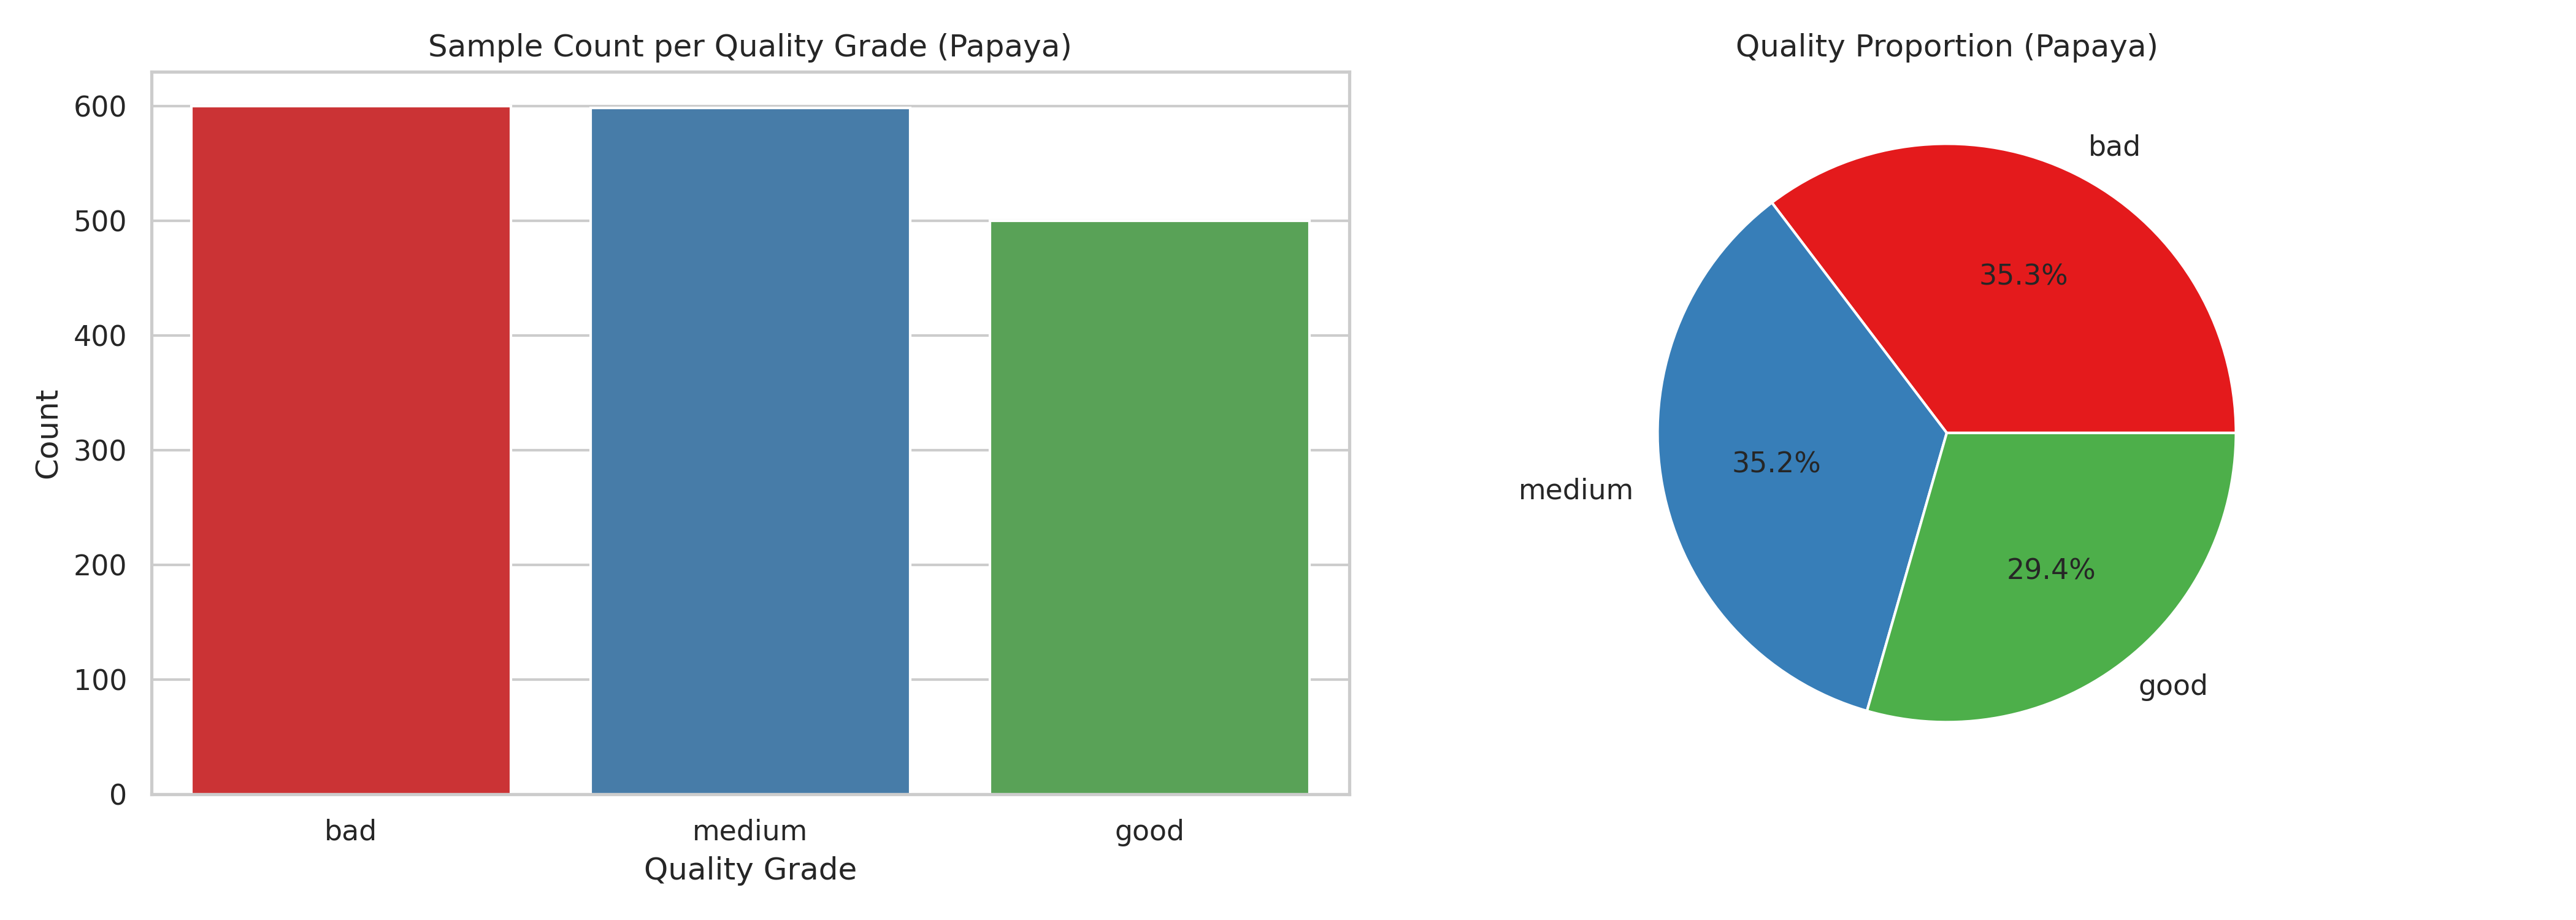
\includegraphics[width=0.85\textwidth]{Output/papaya/fruit_quality_outputs_papaya/plots/papaya_distribution.png}
    \caption{Papaya: Quality class distribution}
    \label{fig:papaya-dist}
\end{figure}

\begin{figure}[H]
    \centering
    
\includegraphics[width=0.85\textwidth]{Output/papaya/fruit_quality_outputs_papaya/plots/final_quality_benchmark_comparison.png}
    \caption{Papaya: Model benchmark comparison}
    \label{fig:papaya-benchmark}
\end{figure}

\begin{figure}[H]
    \centering
    
\includegraphics[width=0.85\textwidth]{Output/papaya/fruit_quality_outputs_papaya/plots/mobilenetv3_large_confusion_matrix_and_roc.png}
    \caption{Papaya: MobileNetV3-Large (top model, 85.59\% accuracy) -- Confusion matrix and ROC curve}
    \label{fig:papaya-cm}
\end{figure}

\begin{figure}[H]
    \centering
    
\includegraphics[width=0.85\textwidth]{Output/papaya/fruit_quality_outputs_papaya/plots/mobilenetv3_large_learning_curves.png}
    \caption{Papaya: MobileNetV3-Large -- Training and validation curves}
    \label{fig:papaya-lc}
\end{figure}

\begin{figure}[H]
    \centering
    
\includegraphics[width=0.85\textwidth]{Output/papaya/fruit_quality_outputs_papaya/plots/mobilenetv3_large_correct_predictions.png}
    \caption{Papaya: MobileNetV3-Large -- Representative correct quality predictions with confidence scores}
    \label{fig:papaya-correct}
\end{figure}

\begin{figure}[H]
    \centering
    
\includegraphics[width=0.85\textwidth]{Output/papaya/fruit_quality_outputs_papaya/plots/mobilenetv3_large_wrong_predictions.png}
    \caption{Papaya: MobileNetV3-Large -- Sample misclassifications and failure case analysis}
    \label{fig:papaya-wrong}
\end{figure}

Papaya remains the \textbf{most challenging} fruit for quality classification across the dataset, with top accuracy reaching 85.59\% on MobileNetV3-Large and 85.29\% on ResNet-50. The difficulty stems from continuous, subtle color and textural transitions between quality grades, particularly the \texttt{medium} category which exhibits high visual overlap with both fresh green-yellow specimens and ripe/blemished surfaces. The Custom CNN baseline achieves 76.18\%, demonstrating that transfer-learning representations provide substantial benefit for resolving complex, multi-scale surface variations. Representative correct quality predictions and failure case diagnostics for MobileNetV3-Large are illustrated in Figure~\ref{fig:papaya-correct} and Figure~\ref{fig:papaya-wrong}.

% ---------- LEMON ----------
\subsection{Lemon}

\begin{table}[H]
\centering\small
\begin{tabular}{@{}lccc@{}}
\toprule
\textbf{Model} & \textbf{Accuracy (\%)} & \textbf{Macro F1} & \textbf{Weighted F1} \\
\midrule
Small Custom CNN & 84.10 & 0.8364 & 0.8402 \\
MobileNetV3-Large & 96.53 & 0.9644 & 0.9653 \\
YOLO26n-cls & 96.24 & 0.9616 & 0.9623 \\
EfficientNet-B0 & 95.95 & 0.9586 & 0.9596 \\
\textbf{ResNet-50} & \textbf{96.82} & \textbf{0.9675} & \textbf{0.9682} \\
\bottomrule
\end{tabular}
\caption{Lemon quality classification benchmark}
\label{tab:lemon-benchmark}
\end{table}

\begin{figure}[H]
    \centering
    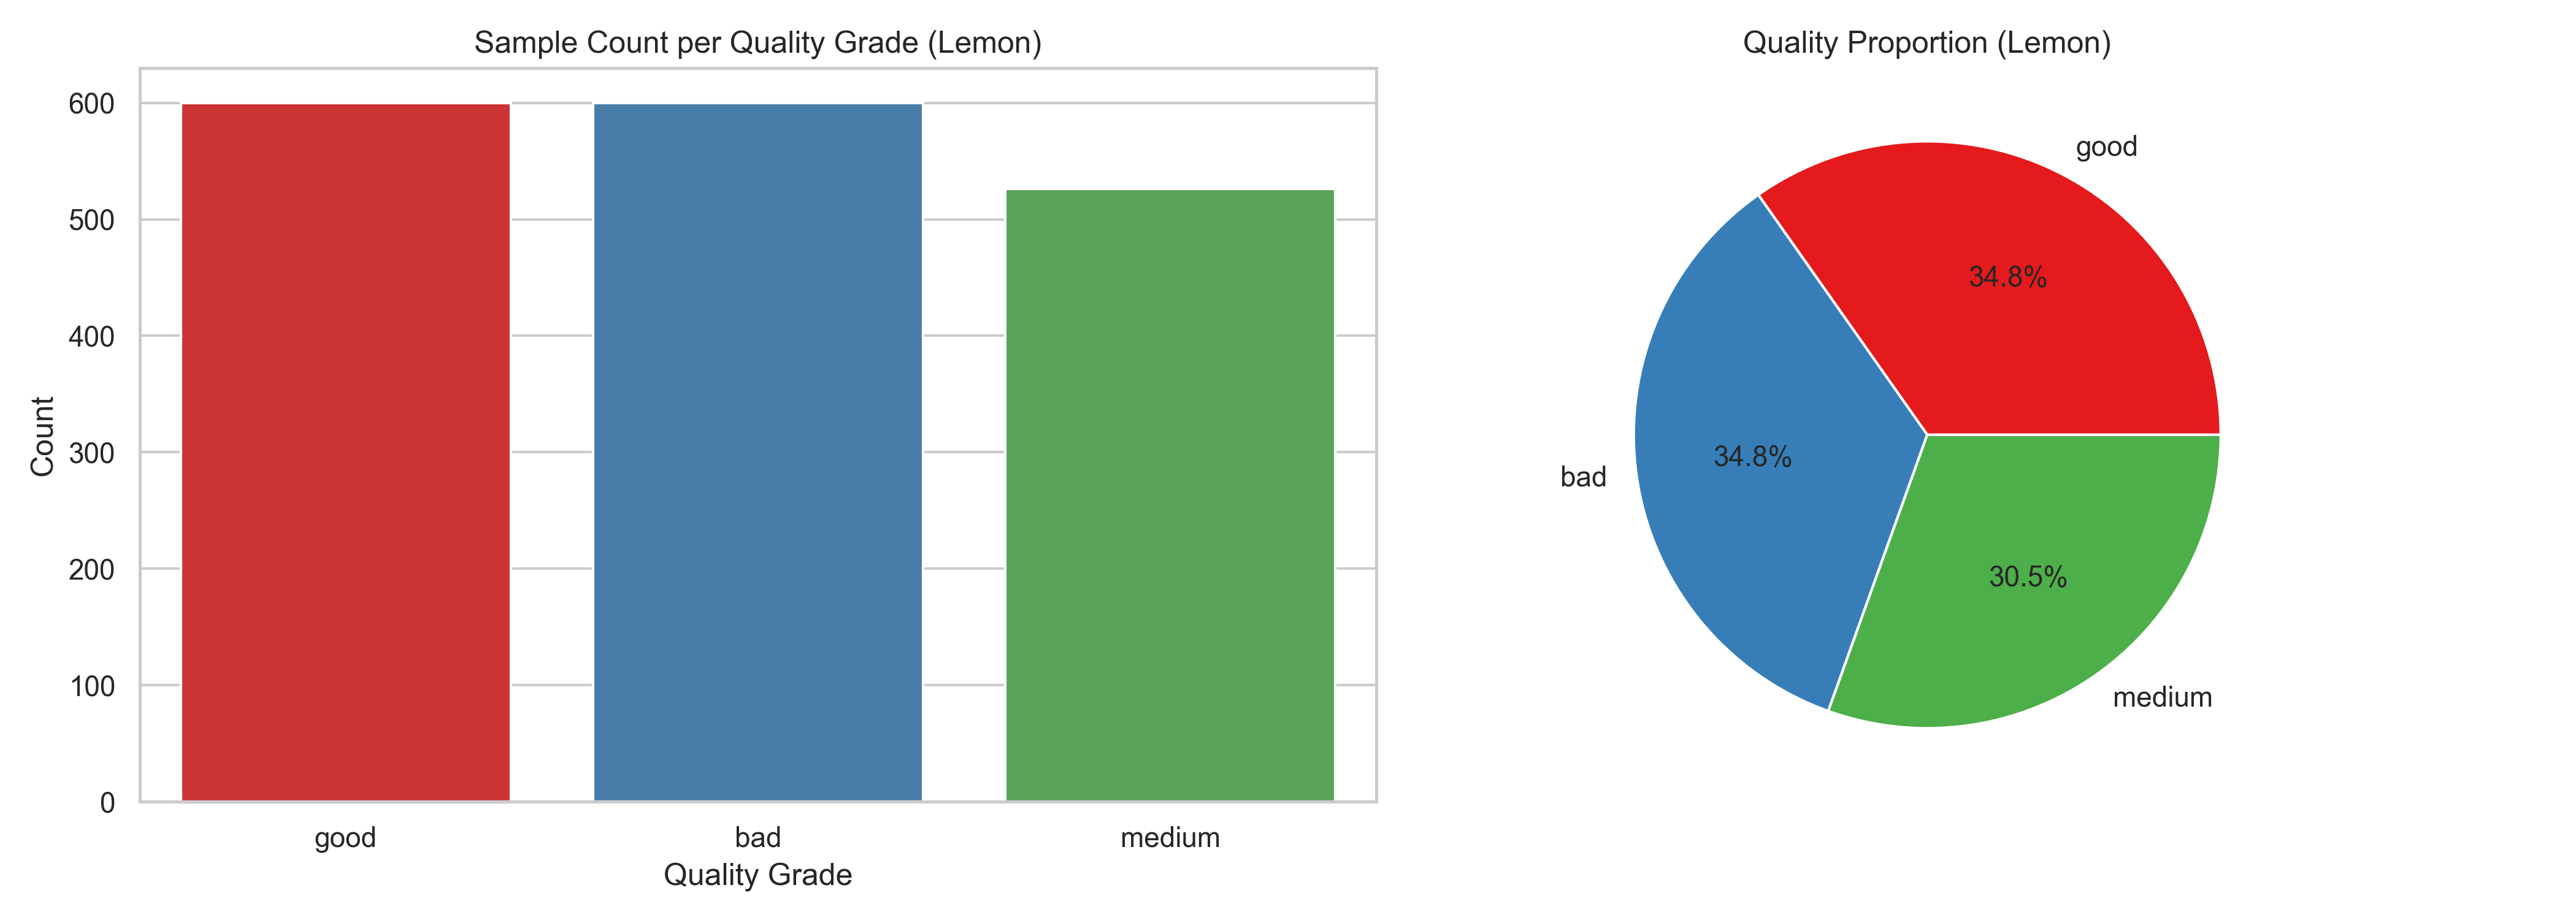
\includegraphics[width=0.85\textwidth]{Output/lemon/fruit_quality_outputs_lemon (1)/plots/lemon_distribution.png}
    \caption{Lemon: Quality class distribution}
    \label{fig:lemon-dist}
\end{figure}

\begin{figure}[H]
    \centering
    
\includegraphics[width=0.85\textwidth]{Output/lemon/fruit_quality_outputs_lemon (1)/plots/final_quality_benchmark_comparison.png}
    \caption{Lemon: Model benchmark comparison}
    \label{fig:lemon-benchmark}
\end{figure}

\begin{figure}[H]
    \centering
    
\includegraphics[width=0.85\textwidth]{Output/lemon/fruit_quality_outputs_lemon (1)/plots/resnet_50_confusion_matrix_and_roc.png}
    \caption{Lemon: ResNet-50 (top model, 96.82\% accuracy) -- Confusion matrix and ROC curve}
    \label{fig:lemon-cm}
\end{figure}

\begin{figure}[H]
    \centering
    
\includegraphics[width=0.85\textwidth]{Output/lemon/fruit_quality_outputs_lemon (1)/plots/resnet_50_learning_curves.png}
    \caption{Lemon: ResNet-50 -- Training and validation curves}
    \label{fig:lemon-lc}
\end{figure}

\begin{figure}[H]
    \centering
    
\includegraphics[width=0.85\textwidth]{Output/lemon/fruit_quality_outputs_lemon (1)/plots/resnet_50_correct_predictions.png}
    \caption{Lemon: ResNet-50 -- Representative correct quality predictions with confidence scores}
    \label{fig:lemon-correct}
\end{figure}

\begin{figure}[H]
    \centering
    
\includegraphics[width=0.85\textwidth]{Output/lemon/fruit_quality_outputs_lemon (1)/plots/resnet_50_wrong_predictions.png}
    \caption{Lemon: ResNet-50 -- Sample misclassifications and failure case analysis}
    \label{fig:lemon-wrong}
\end{figure}

Lemon quality classification achieves strong performance across transfer architectures, led by \textbf{ResNet-50} at 96.82\% accuracy (0.9675 macro F1) and MobileNetV3-Large at 96.53\%. Distinct color shifts from dark green to vibrant yellow and unmistakable surface mold spots provide strong discriminative cues. The Custom CNN reaches 84.10\% accuracy, reflecting a notable 12.7\% performance gap that pre-trained residual representations bridge effectively. Figure~\ref{fig:lemon-correct} shows robust high-confidence classifications across peel stages, while Figure~\ref{fig:lemon-wrong} analyzes the rare error cases arising from borderline green-yellow transitions.

% ---------- LYCHEE ----------
\subsection{Lychee}

\begin{table}[H]
\centering\small
\begin{tabular}{@{}lccc@{}}
\toprule
\textbf{Model} & \textbf{Accuracy (\%)} & \textbf{Macro F1} & \textbf{Weighted F1} \\
\midrule
Small Custom CNN & 99.06 & 0.9907 & 0.9906 \\
\textbf{MobileNetV3-Large} & \textbf{100.00} & \textbf{1.0000} & \textbf{1.0000} \\
\textbf{YOLO26n-cls} & \textbf{100.00} & \textbf{1.0000} & \textbf{1.0000} \\
\textbf{EfficientNet-B0} & \textbf{100.00} & \textbf{1.0000} & \textbf{1.0000} \\
\textbf{ResNet-50} & \textbf{100.00} & \textbf{1.0000} & \textbf{1.0000} \\
\bottomrule
\end{tabular}
\caption{Lychee quality classification benchmark}
\label{tab:lychee-benchmark}
\end{table}

\begin{figure}[H]
    \centering
    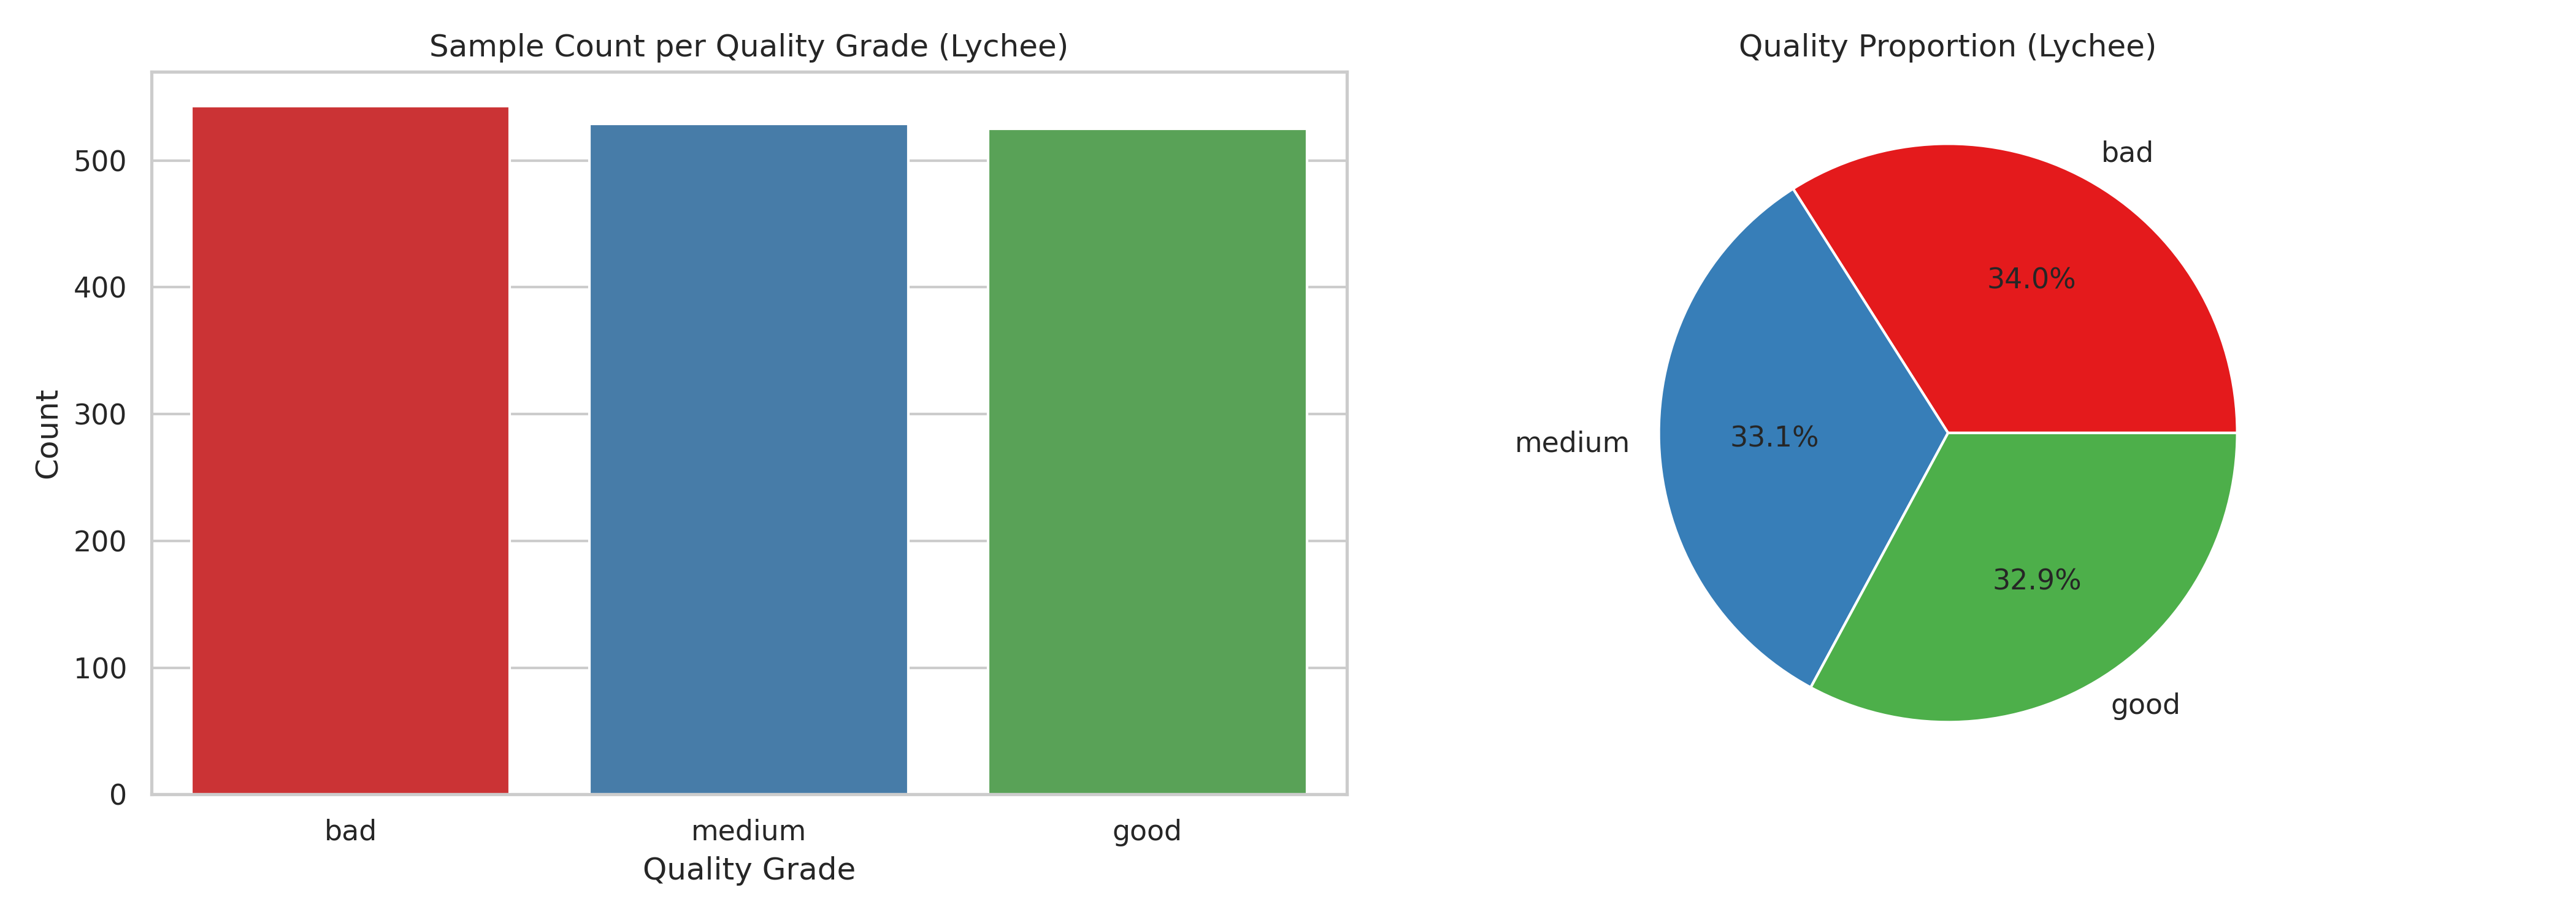
\includegraphics[width=0.85\textwidth]{Output/lychee/fruit_quality_outputs_lychee/plots/lychee_distribution.png}
    \caption{Lychee: Quality class distribution}
    \label{fig:lychee-dist}
\end{figure}

\begin{figure}[H]
    \centering
    
\includegraphics[width=0.85\textwidth]{Output/lychee/fruit_quality_outputs_lychee/plots/final_quality_benchmark_comparison.png}
    \caption{Lychee: Model benchmark comparison}
    \label{fig:lychee-benchmark}
\end{figure}

\begin{figure}[H]
    \centering
    
\includegraphics[width=0.85\textwidth]{Output/lychee/fruit_quality_outputs_lychee/plots/efficientnet_b0_confusion_matrix_and_roc.png}
    \caption{Lychee: EfficientNet-B0 (top model, 100.00\% accuracy) -- Confusion matrix and ROC curve}
    \label{fig:lychee-cm}
\end{figure}

\begin{figure}[H]
    \centering
    
\includegraphics[width=0.85\textwidth]{Output/lychee/fruit_quality_outputs_lychee/plots/efficientnet_b0_learning_curves.png}
    \caption{Lychee: EfficientNet-B0 -- Training and validation curves}
    \label{fig:lychee-lc}
\end{figure}

\begin{figure}[H]
    \centering
    
\includegraphics[width=0.85\textwidth]{Output/lychee/fruit_quality_outputs_lychee/plots/efficientnet_b0_correct_predictions.png}
    \caption{Lychee: EfficientNet-B0 -- Representative correct quality predictions with confidence scores}
    \label{fig:lychee-correct}
\end{figure}

\begin{figure}[H]
    \centering
    
\includegraphics[width=0.85\textwidth]{Output/lychee/fruit_quality_outputs_lychee/plots/efficientnet_b0_wrong_predictions.png}
    \caption{Lychee: EfficientNet-B0 -- Misclassified quality predictions analysis (flawless 100\% test set accuracy)}
    \label{fig:lychee-wrong}
\end{figure}

Lychee quality classification achieves \textbf{flawless 100.00\% accuracy} across all four transfer-learning backbones (MobileNetV3-Large, YOLO26n-cls, EfficientNet-B0, and ResNet-50), with macro and weighted F1-scores of 1.0000. Even the Small Custom CNN baseline performs exceptionally well at 99.06\%. The distinctive visual indicators of lychee deterioration---transitioning from bright red pericarp to brown, desiccated shells---provide unambiguous features that enable complete class separation. Figure~\ref{fig:lychee-correct} and Figure~\ref{fig:lychee-wrong} demonstrate the high prediction confidence of EfficientNet-B0 and confirm zero test-set misclassifications.

% ---------- JACKFRUIT ----------
\subsection{Jackfruit}

\begin{table}[H]
\centering\small
\begin{tabular}{@{}lccc@{}}
\toprule
\textbf{Model} & \textbf{Accuracy (\%)} & \textbf{Macro F1} & \textbf{Weighted F1} \\
\midrule
Small Custom CNN & 76.49 & 0.7658 & 0.7661 \\
\textbf{MobileNetV3-Large} & \textbf{99.67} & \textbf{0.9967} & \textbf{0.9967} \\
YOLO26n-cls & 97.68 & 0.9768 & 0.9768 \\
\textbf{EfficientNet-B0} & \textbf{99.67} & \textbf{0.9967} & \textbf{0.9967} \\
ResNet-50 & 99.34 & 0.9934 & 0.9934 \\
\bottomrule
\end{tabular}
\caption{Jackfruit quality classification benchmark}
\label{tab:jackfruit-benchmark}
\end{table}

\begin{figure}[H]
    \centering
    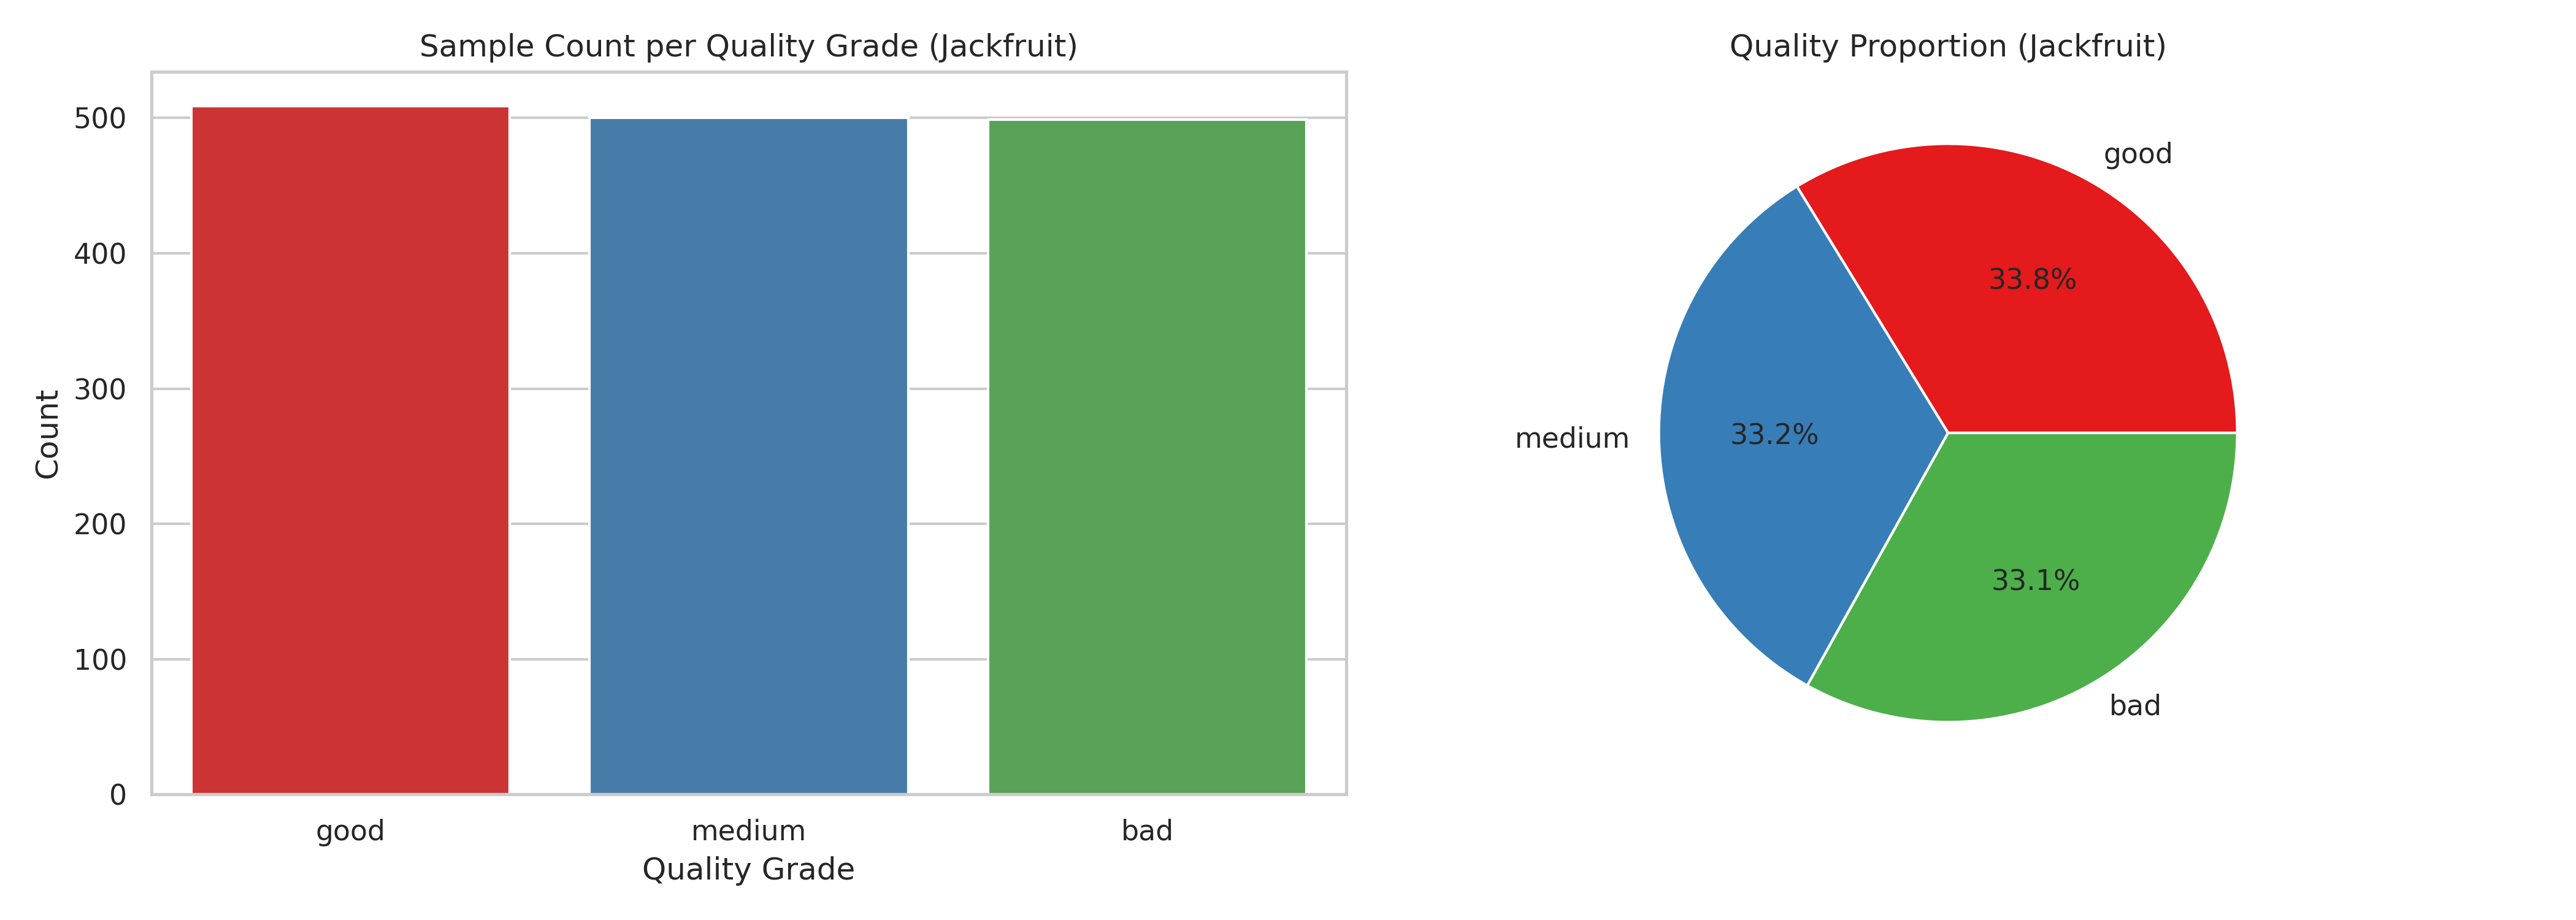
\includegraphics[width=0.85\textwidth]{Output/jackfruit/fruit_quality_outputs_jackfruit/plots/jackfruit_distribution.png}
    \caption{Jackfruit: Quality class distribution}
    \label{fig:jackfruit-dist}
\end{figure}

\begin{figure}[H]
    \centering
    
\includegraphics[width=0.85\textwidth]{Output/jackfruit/fruit_quality_outputs_jackfruit/plots/final_quality_benchmark_comparison.png}
    \caption{Jackfruit: Model benchmark comparison}
    \label{fig:jackfruit-benchmark}
\end{figure}

\begin{figure}[H]
    \centering
    
\includegraphics[width=0.85\textwidth]{Output/jackfruit/fruit_quality_outputs_jackfruit/plots/mobilenetv3_large_confusion_matrix_and_roc.png}
    \caption{Jackfruit: MobileNetV3-Large (top model, 99.67\% accuracy) -- Confusion matrix and ROC curve}
    \label{fig:jackfruit-cm}
\end{figure}

\begin{figure}[H]
    \centering
    
\includegraphics[width=0.85\textwidth]{Output/jackfruit/fruit_quality_outputs_jackfruit/plots/mobilenetv3_large_learning_curves.png}
    \caption{Jackfruit: MobileNetV3-Large -- Training and validation curves}
    \label{fig:jackfruit-lc}
\end{figure}

\begin{figure}[H]
    \centering
    
\includegraphics[width=0.85\textwidth]{Output/jackfruit/fruit_quality_outputs_jackfruit/plots/mobilenetv3_large_correct_predictions.png}
    \caption{Jackfruit: MobileNetV3-Large -- Representative correct quality predictions with confidence scores}
    \label{fig:jackfruit-correct}
\end{figure}

\begin{figure}[H]
    \centering
    
\includegraphics[width=0.85\textwidth]{Output/jackfruit/fruit_quality_outputs_jackfruit/plots/mobilenetv3_large_wrong_predictions.png}
    \caption{Jackfruit: MobileNetV3-Large -- Sample misclassifications and failure case analysis}
    \label{fig:jackfruit-wrong}
\end{figure}

Jackfruit quality classification demonstrates outstanding accuracy, with both \textbf{MobileNetV3-Large} and \textbf{EfficientNet-B0} achieving 99.67\% accuracy (0.9967 macro F1) and ResNet-50 reaching 99.34\%. In contrast, the Custom CNN baseline struggles at 76.49\% accuracy, highlighting a substantial 23.2\% margin that underscores the necessity of rich, pre-trained spatial hierarchies for interpreting complex spiky exterior textures. Figure~\ref{fig:jackfruit-correct} and Figure~\ref{fig:jackfruit-wrong} illustrate prediction samples and error diagnostics on textured jackfruit surfaces.

% ---------- MANGO ----------
\subsection{Mango}

\begin{table}[H]
\centering\small
\begin{tabular}{@{}lccc@{}}
\toprule
\textbf{Model} & \textbf{Accuracy (\%)} & \textbf{Macro F1} & \textbf{Weighted F1} \\
\midrule
Small Custom CNN & 85.31 & 0.8533 & 0.8541 \\
\textbf{MobileNetV3-Large} & \textbf{94.38} & \textbf{0.9425} & \textbf{0.9433} \\
\textbf{YOLO26n-cls} & \textbf{94.38} & \textbf{0.9431} & \textbf{0.9437} \\
EfficientNet-B0 & 92.81 & 0.9271 & 0.9280 \\
ResNet-50 & 92.50 & 0.9245 & 0.9251 \\
\bottomrule
\end{tabular}
\caption{Mango quality classification benchmark}
\label{tab:mango-benchmark}
\end{table}

\begin{figure}[H]
    \centering
    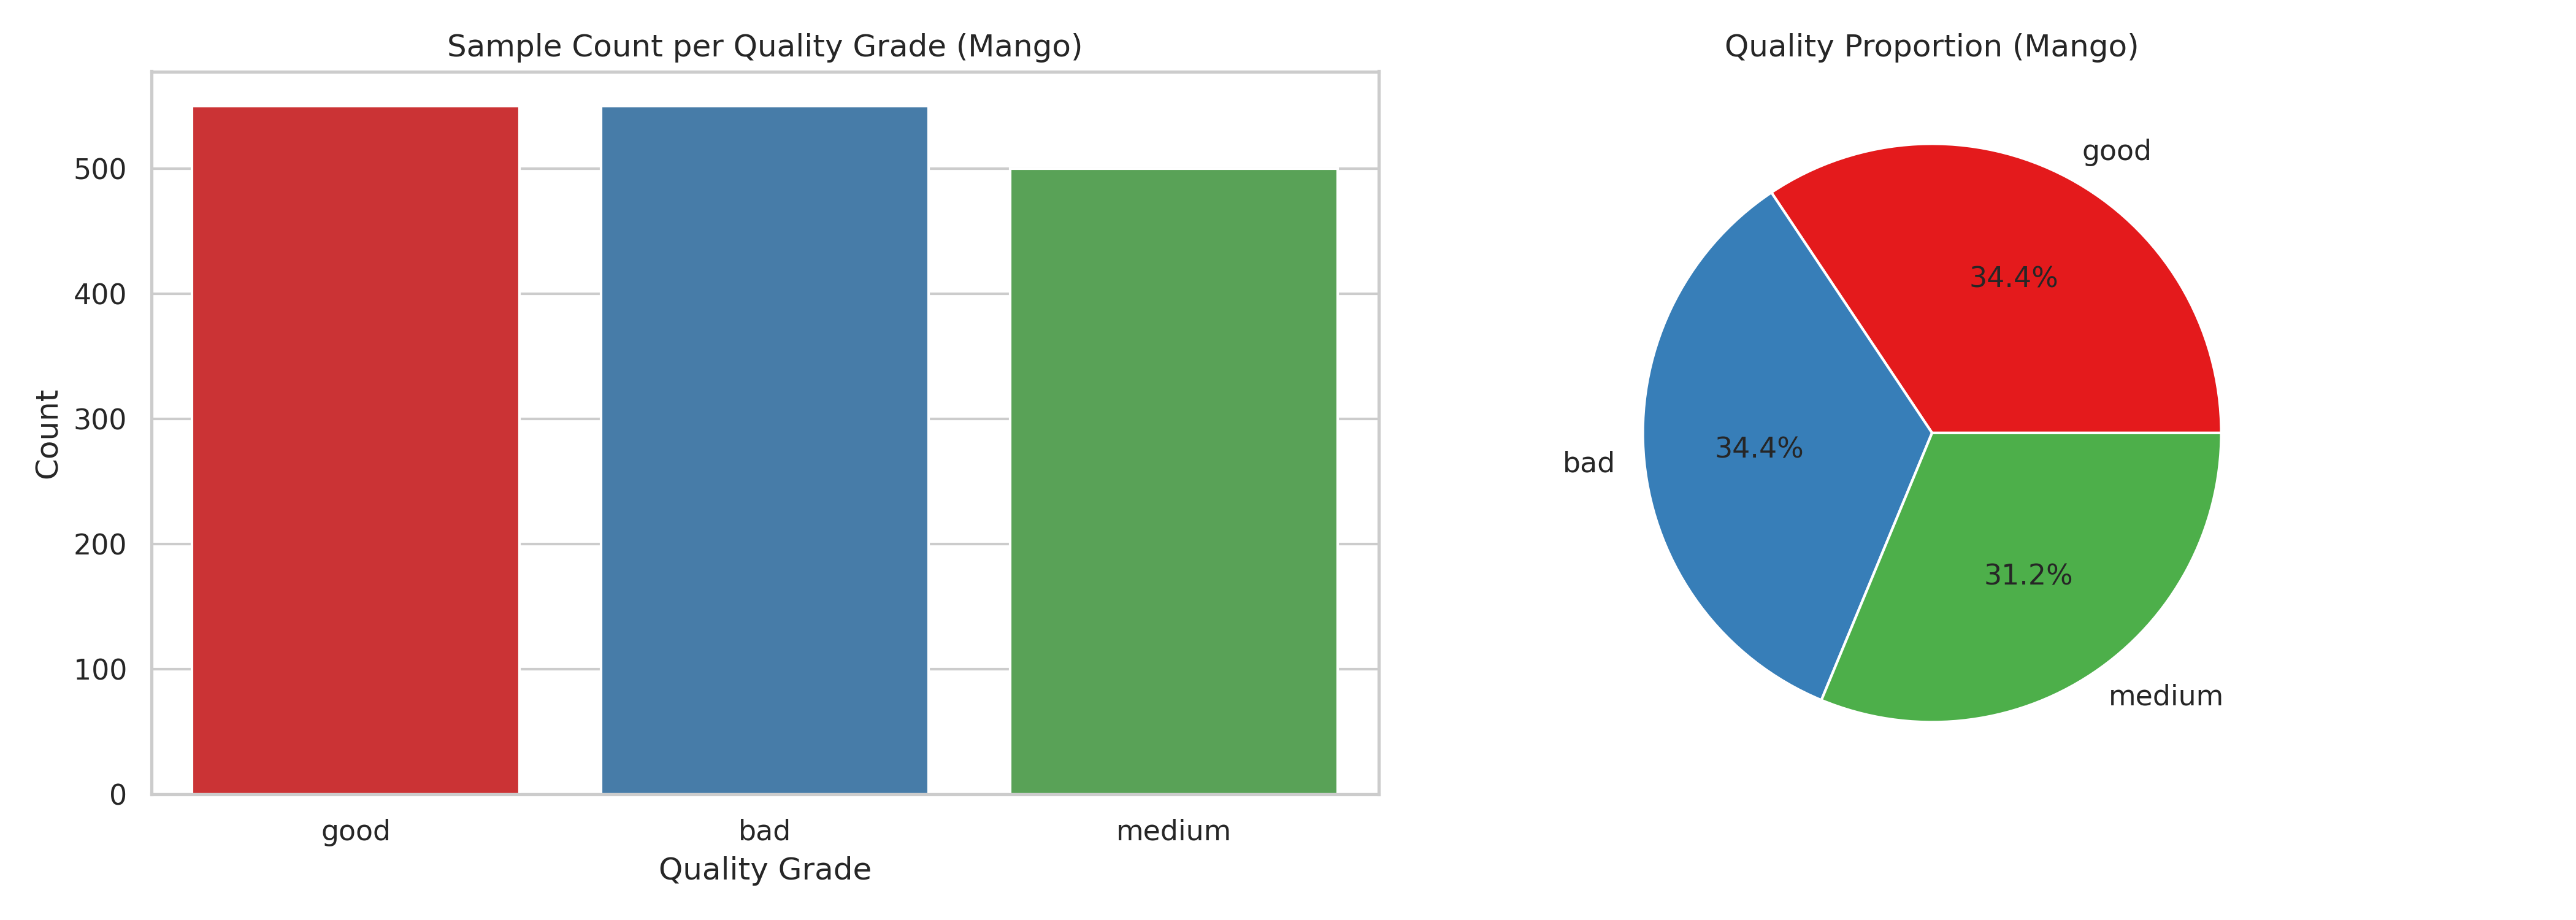
\includegraphics[width=0.85\textwidth]{Output/mango/fruit_quality_outputs_mango/plots/mango_distribution.png}
    \caption{Mango: Quality class distribution}
    \label{fig:mango-dist}
\end{figure}

\begin{figure}[H]
    \centering
    
\includegraphics[width=0.85\textwidth]{Output/mango/fruit_quality_outputs_mango/plots/final_quality_benchmark_comparison.png}
    \caption{Mango: Model benchmark comparison}
    \label{fig:mango-benchmark}
\end{figure}

\begin{figure}[H]
    \centering
    
\includegraphics[width=0.85\textwidth]{Output/mango/fruit_quality_outputs_mango/plots/mobilenetv3_large_confusion_matrix_and_roc.png}
    \caption{Mango: MobileNetV3-Large (top model, 94.38\% accuracy) -- Confusion matrix and ROC curve}
    \label{fig:mango-cm}
\end{figure}

\begin{figure}[H]
    \centering
    
\includegraphics[width=0.85\textwidth]{Output/mango/fruit_quality_outputs_mango/plots/mobilenetv3_large_learning_curves.png}
    \caption{Mango: MobileNetV3-Large -- Training and validation curves}
    \label{fig:mango-lc}
\end{figure}

\begin{figure}[H]
    \centering
    
\includegraphics[width=0.85\textwidth]{Output/mango/fruit_quality_outputs_mango/plots/mobilenetv3_large_correct_predictions.png}
    \caption{Mango: MobileNetV3-Large -- Representative correct quality predictions with confidence scores}
    \label{fig:mango-correct}
\end{figure}

\begin{figure}[H]
    \centering
    
\includegraphics[width=0.85\textwidth]{Output/mango/fruit_quality_outputs_mango/plots/mobilenetv3_large_wrong_predictions.png}
    \caption{Mango: MobileNetV3-Large -- Sample misclassifications and failure case analysis}
    \label{fig:mango-wrong}
\end{figure}

For mango quality classification, \textbf{MobileNetV3-Large} and \textbf{YOLO26n-cls} both achieve the top accuracy of 94.38\% (0.9425 and 0.9431 macro F1, respectively), while EfficientNet-B0 and ResNet-50 achieve 92.81\% and 92.50\%. The Custom CNN baseline reaches 85.31\%. Subtle ripening spots (lenticels) and natural skin blushing create moderate confusion between \texttt{good} and \texttt{medium} grades, whereas decayed specimens (\texttt{bad}) are detected with near-perfect sensitivity. Figure~\ref{fig:mango-correct} and Figure~\ref{fig:mango-wrong} visualize representative correct predictions and sample failure cases for MobileNetV3-Large.

% ---------- STAR FRUIT ----------
\subsection{Star Fruit}

\begin{table}[H]
\centering\small
\begin{tabular}{@{}lccc@{}}
\toprule
\textbf{Model} & \textbf{Accuracy (\%)} & \textbf{Macro F1} & \textbf{Weighted F1} \\
\midrule
Small Custom CNN & 80.00 & 0.7909 & 0.7939 \\
\textbf{MobileNetV3-Large} & \textbf{92.19} & \textbf{0.9184} & \textbf{0.9200} \\
YOLO26n-cls & 89.06 & 0.8881 & 0.8899 \\
EfficientNet-B0 & 90.00 & 0.8970 & 0.8988 \\
ResNet-50 & 90.00 & 0.8964 & 0.8981 \\
\bottomrule
\end{tabular}
\caption{Star Fruit quality classification benchmark}
\label{tab:star-benchmark}
\end{table}

\begin{figure}[H]
    \centering
    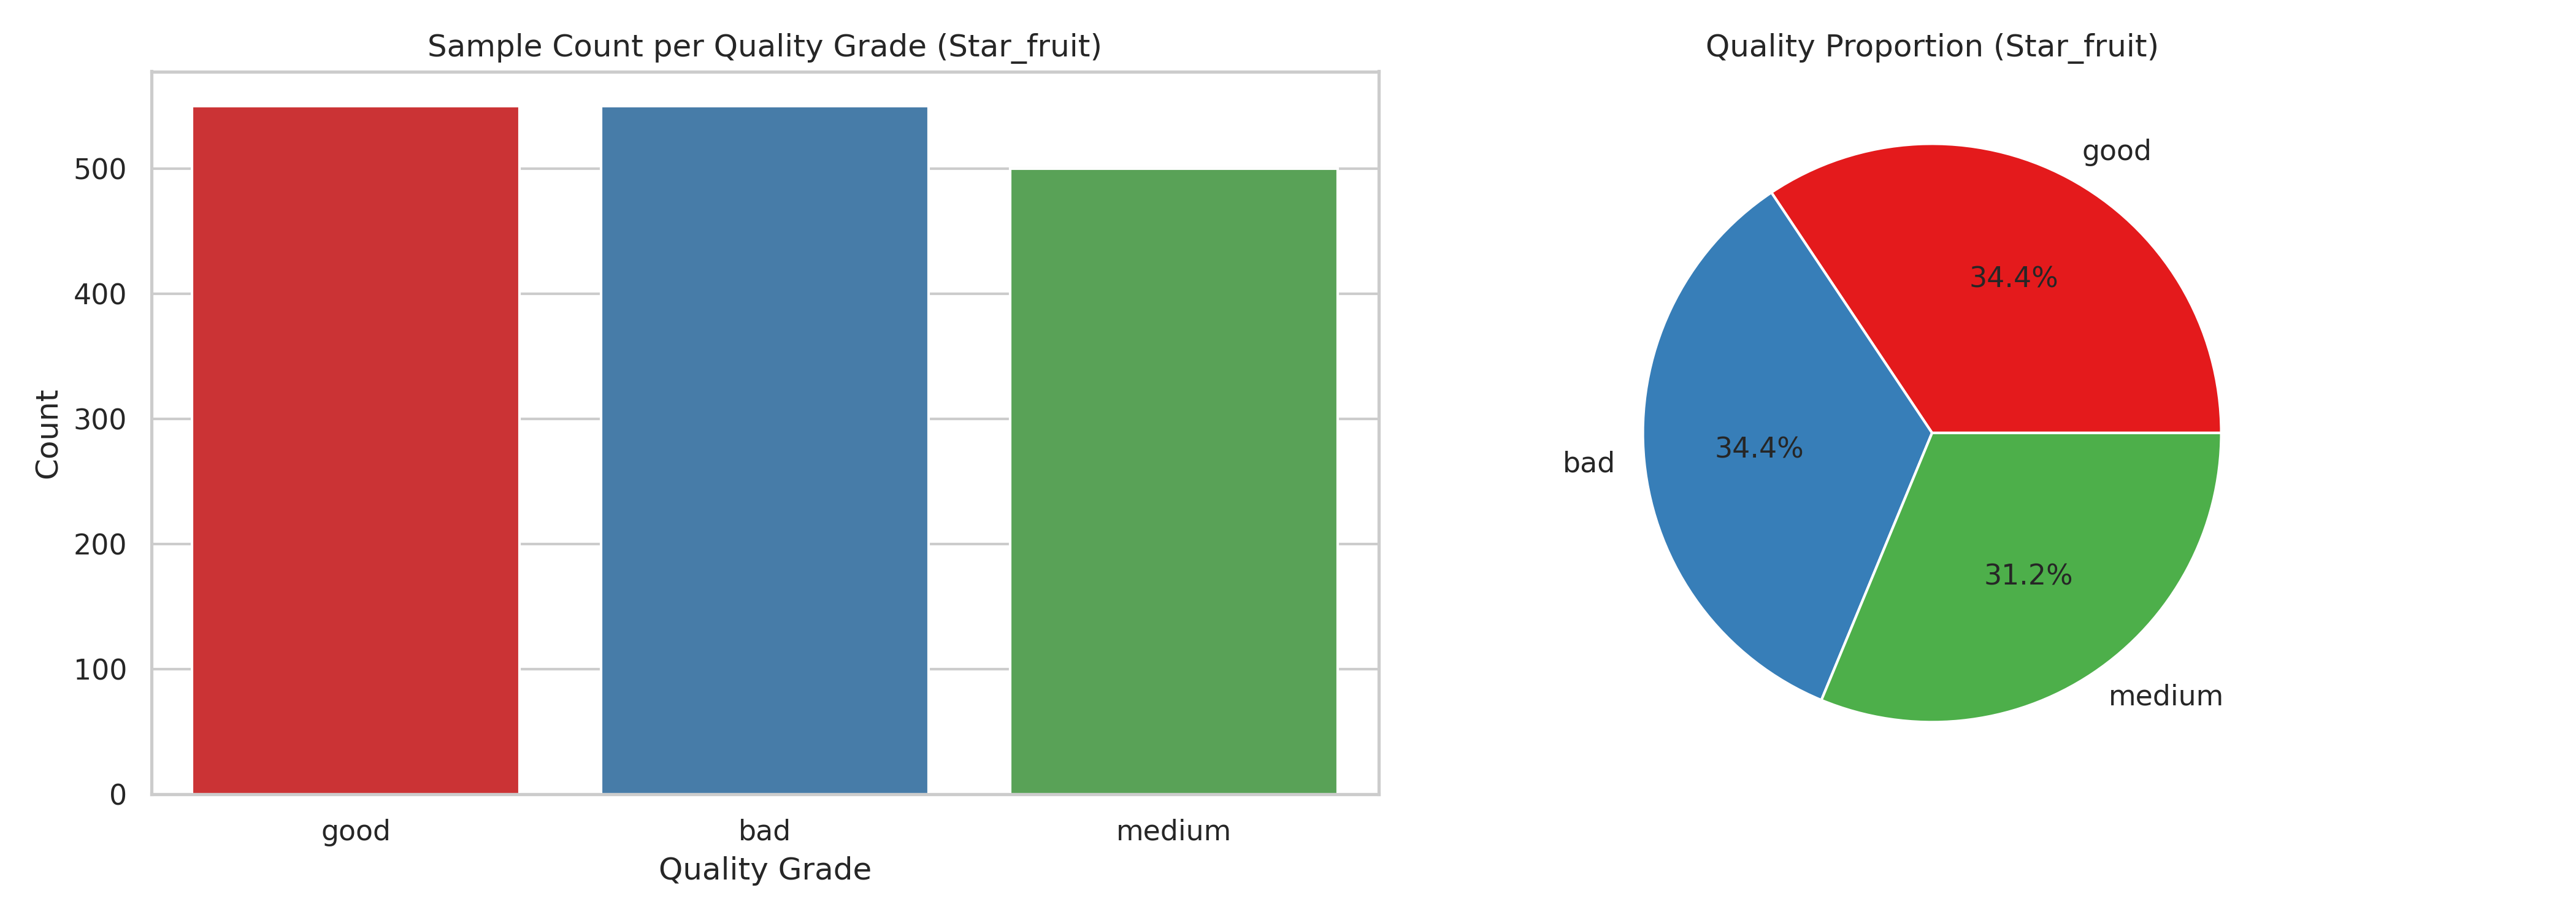
\includegraphics[width=0.85\textwidth]{Output/starfruit/fruit_quality_outputs_star_fruit/plots/star_fruit_distribution.png}
    \caption{Star Fruit: Quality class distribution}
    \label{fig:star-dist}
\end{figure}

\begin{figure}[H]
    \centering
    
\includegraphics[width=0.85\textwidth]{Output/starfruit/fruit_quality_outputs_star_fruit/plots/final_quality_benchmark_comparison.png}
    \caption{Star Fruit: Model benchmark comparison}
    \label{fig:star-benchmark}
\end{figure}

\begin{figure}[H]
    \centering
    
\includegraphics[width=0.85\textwidth]{Output/starfruit/fruit_quality_outputs_star_fruit/plots/mobilenetv3_large_confusion_matrix_and_roc.png}
    \caption{Star Fruit: MobileNetV3-Large (top model, 92.19\% accuracy) -- Confusion matrix and ROC curve}
    \label{fig:star-cm}
\end{figure}

\begin{figure}[H]
    \centering
    
\includegraphics[width=0.85\textwidth]{Output/starfruit/fruit_quality_outputs_star_fruit/plots/mobilenetv3_large_learning_curves.png}
    \caption{Star Fruit: MobileNetV3-Large -- Training and validation curves}
    \label{fig:star-lc}
\end{figure}

\begin{figure}[H]
    \centering
    
\includegraphics[width=0.85\textwidth]{Output/starfruit/fruit_quality_outputs_star_fruit/plots/mobilenetv3_large_correct_predictions.png}
    \caption{Star Fruit: MobileNetV3-Large -- Representative correct quality predictions with confidence scores}
    \label{fig:star-correct}
\end{figure}

\begin{figure}[H]
    \centering
    
\includegraphics[width=0.85\textwidth]{Output/starfruit/fruit_quality_outputs_star_fruit/plots/mobilenetv3_large_wrong_predictions.png}
    \caption{Star Fruit: MobileNetV3-Large -- Sample misclassifications and failure case analysis}
    \label{fig:star-wrong}
\end{figure}

Star fruit quality inspection reaches its highest accuracy of 92.19\% (0.9184 macro F1) with \textbf{MobileNetV3-Large}, while EfficientNet-B0 and ResNet-50 achieve 90.00\%, and YOLO26n-cls reaches 89.06\%. The Small Custom CNN achieves 80.00\%. The five-angled geometry of carambola creates localized rib-edge browning that can be challenging to differentiate between intermediate ripening and early decay. Figure~\ref{fig:star-correct} and Figure~\ref{fig:star-wrong} provide visual insights into MobileNetV3-Large predictions and failure modes along the prominent rib contours.

% ---------- GUAVA ----------
\subsection{Guava}

\begin{table}[H]
\centering\small
\begin{tabular}{@{}lccc@{}}
\toprule
\textbf{Model} & \textbf{Accuracy (\%)} & \textbf{Macro F1} & \textbf{Weighted F1} \\
\midrule
Small Custom CNN & 97.21 & 0.9725 & 0.9721 \\
MobileNetV3-Large & 99.07 & 0.9905 & 0.9907 \\
\textbf{YOLO26n-cls} & \textbf{99.38} & \textbf{0.9936} & \textbf{0.9938} \\
\textbf{EfficientNet-B0} & \textbf{99.38} & \textbf{0.9936} & \textbf{0.9938} \\
ResNet-50 & 99.07 & 0.9905 & 0.9907 \\
\bottomrule
\end{tabular}
\caption{Guava quality classification benchmark}
\label{tab:guava-benchmark}
\end{table}

\begin{figure}[H]
    \centering
    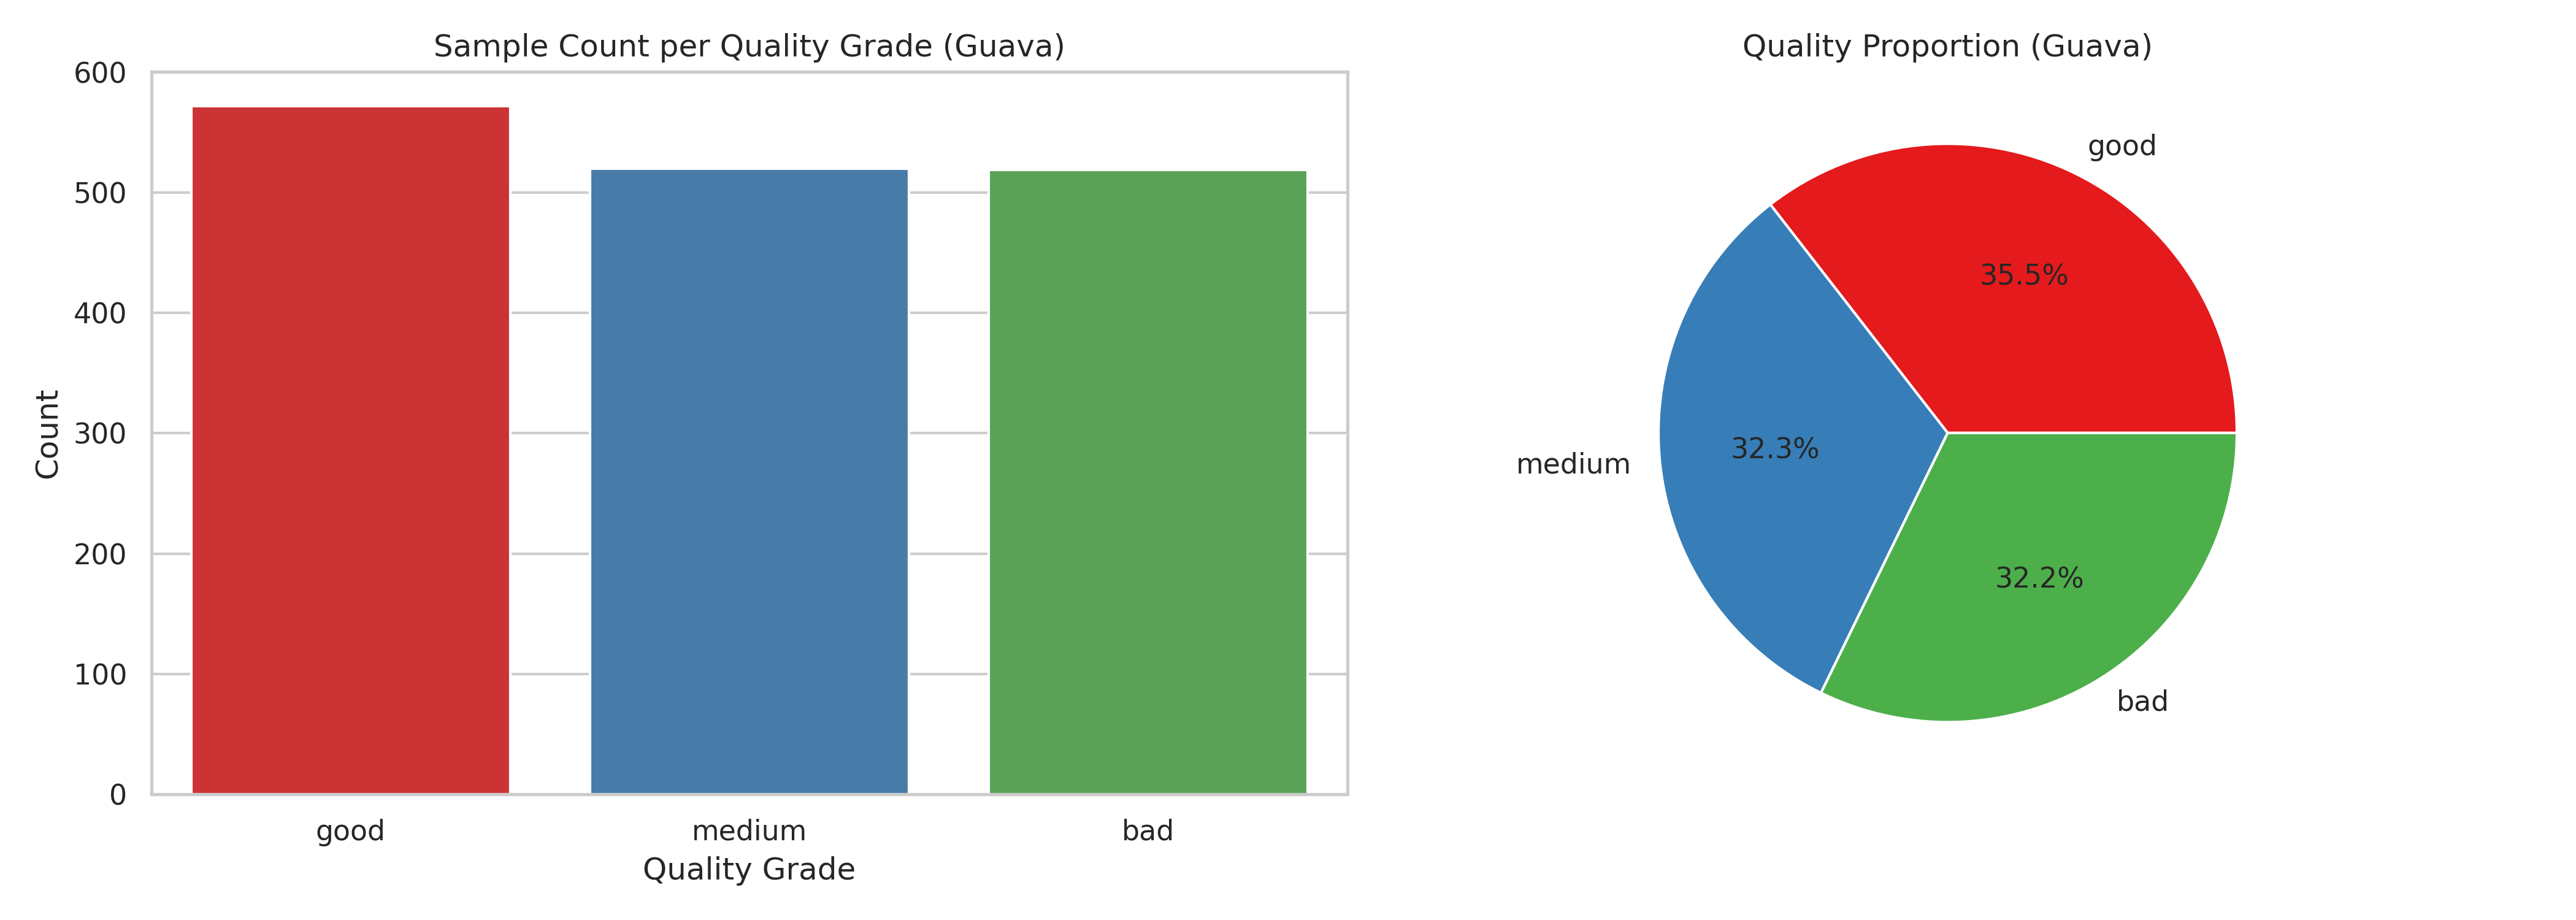
\includegraphics[width=0.85\textwidth]{Output/guava/fruit_quality_outputs_guava/plots/guava_distribution.png}
    \caption{Guava: Quality class distribution}
    \label{fig:guava-dist}
\end{figure}

\begin{figure}[H]
    \centering
    
\includegraphics[width=0.85\textwidth]{Output/guava/fruit_quality_outputs_guava/plots/final_quality_benchmark_comparison.png}
    \caption{Guava: Model benchmark comparison}
    \label{fig:guava-benchmark}
\end{figure}

\begin{figure}[H]
    \centering
    
\includegraphics[width=0.85\textwidth]{Output/guava/fruit_quality_outputs_guava/plots/efficientnet_b0_confusion_matrix_and_roc.png}
    \caption{Guava: EfficientNet-B0 (top model, 99.38\% accuracy) -- Confusion matrix and ROC curve}
    \label{fig:guava-cm}
\end{figure}

\begin{figure}[H]
    \centering
    
\includegraphics[width=0.85\textwidth]{Output/guava/fruit_quality_outputs_guava/plots/efficientnet_b0_learning_curves.png}
    \caption{Guava: EfficientNet-B0 -- Training and validation curves}
    \label{fig:guava-lc}
\end{figure}

\begin{figure}[H]
    \centering
    
\includegraphics[width=0.85\textwidth]{Output/guava/fruit_quality_outputs_guava/plots/efficientnet_b0_correct_predictions.png}
    \caption{Guava: EfficientNet-B0 -- Representative correct quality predictions with confidence scores}
    \label{fig:guava-correct}
\end{figure}

\begin{figure}[H]
    \centering
    
\includegraphics[width=0.85\textwidth]{Output/guava/fruit_quality_outputs_guava/plots/efficientnet_b0_wrong_predictions.png}
    \caption{Guava: EfficientNet-B0 -- Sample misclassifications and failure case analysis}
    \label{fig:guava-wrong}
\end{figure}

Guava quality classification achieves exceptional discrimination, with both \textbf{EfficientNet-B0} and \textbf{YOLO26n-cls} reaching 99.38\% accuracy (0.9936 macro F1), closely followed by MobileNetV3-Large and ResNet-50 at 99.07\%. The Small Custom CNN baseline also delivers high performance at 97.21\%. The clear contrast between smooth green skin, localized scab spots, and extensive soft rot enables near-perfect separation. Figure~\ref{fig:guava-correct} and Figure~\ref{fig:guava-wrong} display high-confidence predictions and diagnostic error visualizations for EfficientNet-B0.

% ---------- JUJUBE ----------
\subsection{Jujube}

\begin{table}[H]
\centering\small
\begin{tabular}{@{}lccc@{}}
\toprule
\textbf{Model} & \textbf{Accuracy (\%)} & \textbf{Macro F1} & \textbf{Weighted F1} \\
\midrule
Small Custom CNN & 89.32 & 0.8951 & 0.8925 \\
\textbf{MobileNetV3-Large} & \textbf{98.81} & \textbf{0.9884} & \textbf{0.9881} \\
YOLO26n-cls & 97.63 & 0.9768 & 0.9762 \\
\textbf{EfficientNet-B0} & \textbf{98.81} & \textbf{0.9884} & \textbf{0.9881} \\
ResNet-50 & 97.63 & 0.9769 & 0.9763 \\
\bottomrule
\end{tabular}
\caption{Jujube quality classification benchmark}
\label{tab:jujube-benchmark}
\end{table}

\begin{figure}[H]
    \centering
    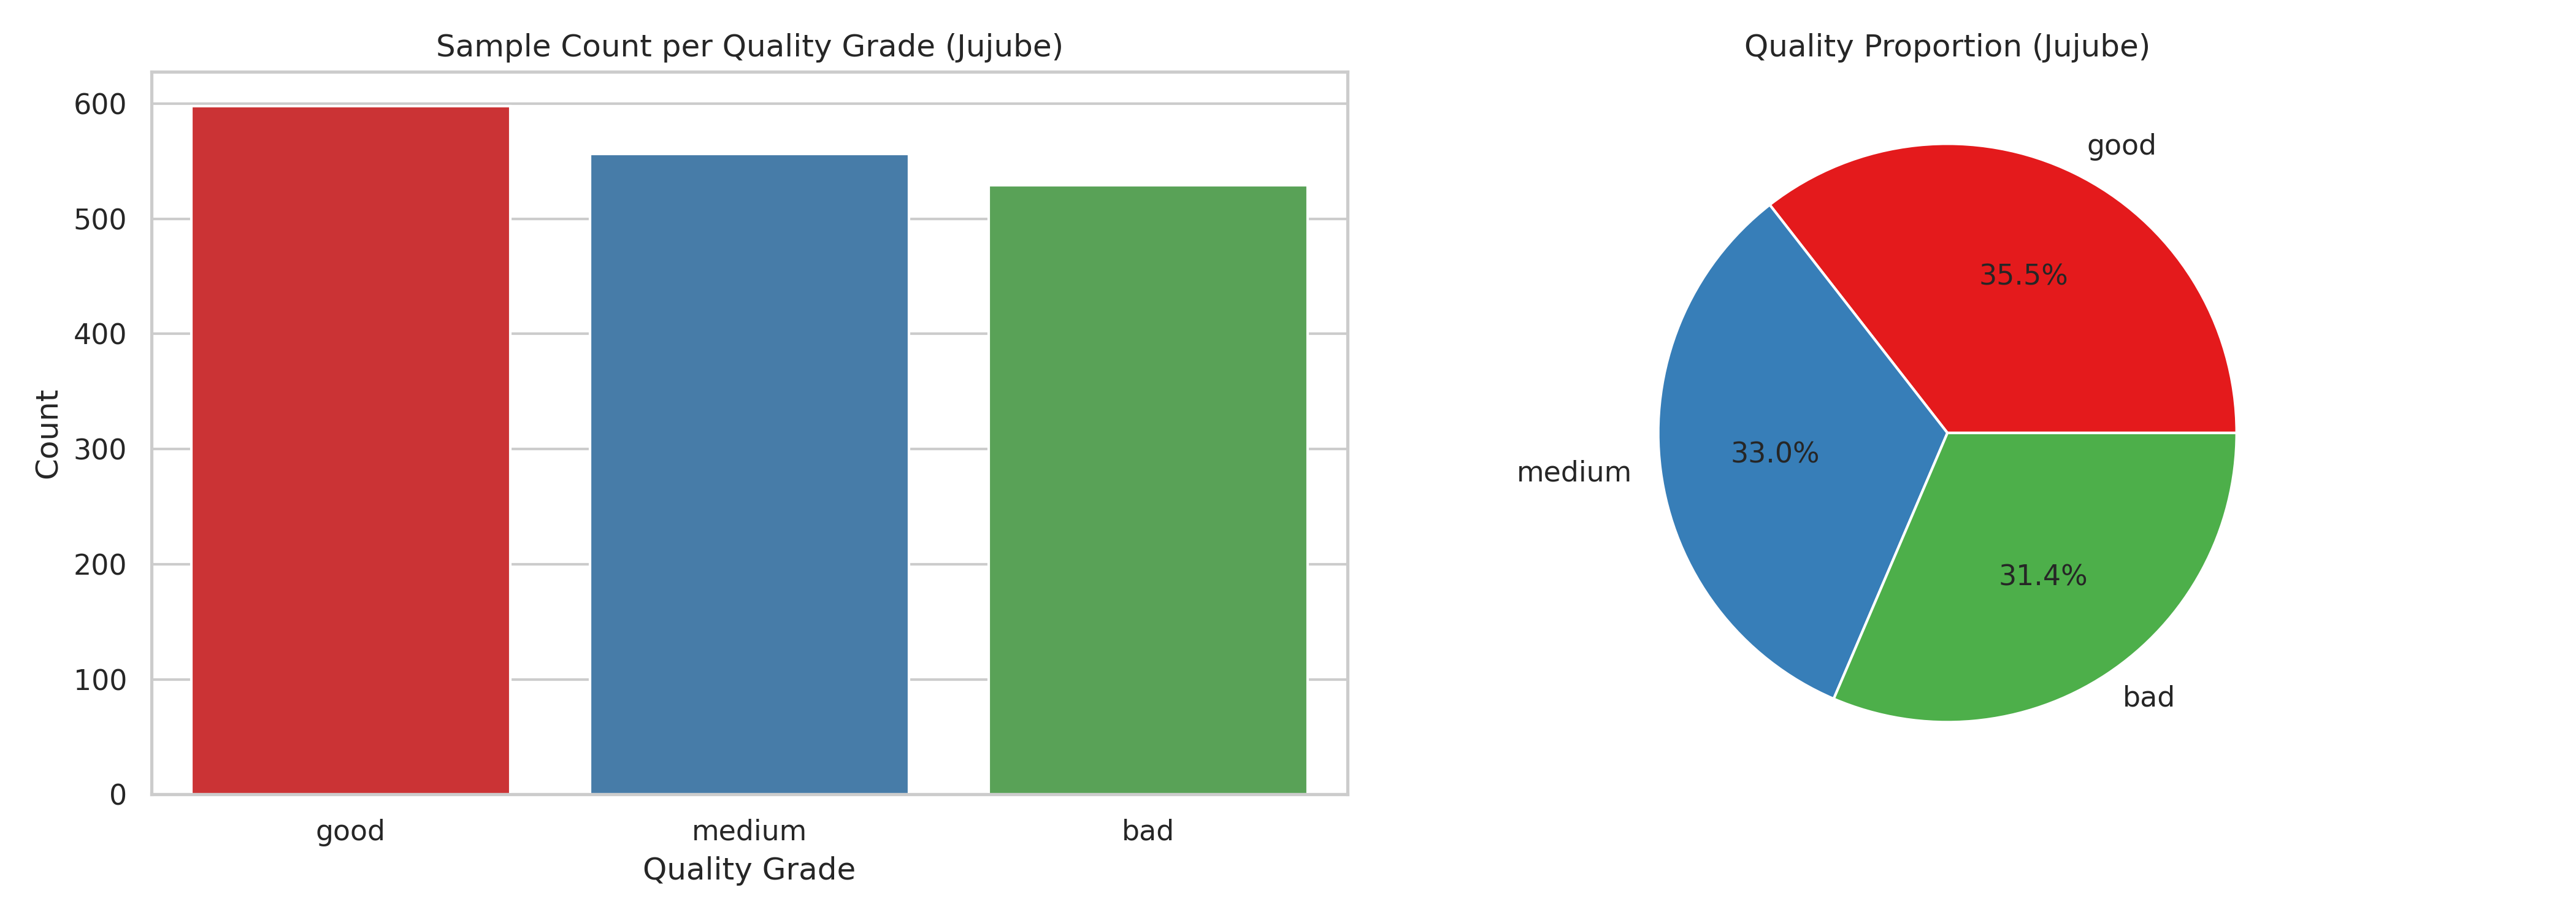
\includegraphics[width=0.85\textwidth]{Output/jujube/fruit_quality_outputs_jujube/plots/jujube_distribution.png}
    \caption{Jujube: Quality class distribution}
    \label{fig:jujube-dist}
\end{figure}

\begin{figure}[H]
    \centering
    
\includegraphics[width=0.85\textwidth]{Output/jujube/fruit_quality_outputs_jujube/plots/final_quality_benchmark_comparison.png}
    \caption{Jujube: Model benchmark comparison}
    \label{fig:jujube-benchmark}
\end{figure}

\begin{figure}[H]
    \centering
    
\includegraphics[width=0.85\textwidth]{Output/jujube/fruit_quality_outputs_jujube/plots/mobilenetv3_large_confusion_matrix_and_roc.png}
    \caption{Jujube: MobileNetV3-Large (top model, 98.81\% accuracy) -- Confusion matrix and ROC curve}
    \label{fig:jujube-cm}
\end{figure}

\begin{figure}[H]
    \centering
    
\includegraphics[width=0.85\textwidth]{Output/jujube/fruit_quality_outputs_jujube/plots/mobilenetv3_large_learning_curves.png}
    \caption{Jujube: MobileNetV3-Large -- Training and validation curves}
    \label{fig:jujube-lc}
\end{figure}

\begin{figure}[H]
    \centering
    
\includegraphics[width=0.85\textwidth]{Output/jujube/fruit_quality_outputs_jujube/plots/mobilenetv3_large_correct_predictions.png}
    \caption{Jujube: MobileNetV3-Large -- Representative correct quality predictions with confidence scores}
    \label{fig:jujube-correct}
\end{figure}

\begin{figure}[H]
    \centering
    
\includegraphics[width=0.85\textwidth]{Output/jujube/fruit_quality_outputs_jujube/plots/mobilenetv3_large_wrong_predictions.png}
    \caption{Jujube: MobileNetV3-Large -- Sample misclassifications and failure case analysis}
    \label{fig:jujube-wrong}
\end{figure}

For jujube quality grading, \textbf{MobileNetV3-Large} and \textbf{EfficientNet-B0} lead the benchmark with 98.81\% accuracy (0.9884 macro F1), while YOLO26n-cls and ResNet-50 achieve 97.63\%. The Custom CNN baseline attains 89.32\%. Deep convolutional features effectively capture the subtle skin wrinkling, red-brown discoloration, and shriveling that distinguish medium-grade and over-mature jujubes from crisp fresh fruit. Figure~\ref{fig:jujube-correct} and Figure~\ref{fig:jujube-wrong} illustrate prediction samples and failure case analysis for MobileNetV3-Large.

% ---------- BANANA ----------
\subsection{Banana}

\begin{table}[H]
\centering\small
\begin{tabular}{@{}lccc@{}}
\toprule
\textbf{Model} & \textbf{Accuracy (\%)} & \textbf{Macro F1} & \textbf{Weighted F1} \\
\midrule
Small Custom CNN & 97.45 & 0.9744 & 0.9746 \\
MobileNetV3-Large & 99.68 & 0.9967 & 0.9968 \\
\textbf{YOLO26n-cls} & \textbf{100.00} & \textbf{1.0000} & \textbf{1.0000} \\
\textbf{EfficientNet-B0} & \textbf{100.00} & \textbf{1.0000} & \textbf{1.0000} \\
ResNet-50 & 99.68 & 0.9967 & 0.9968 \\
\bottomrule
\end{tabular}
\caption{Banana quality classification benchmark}
\label{tab:banana-benchmark}
\end{table}

\begin{figure}[H]
    \centering
    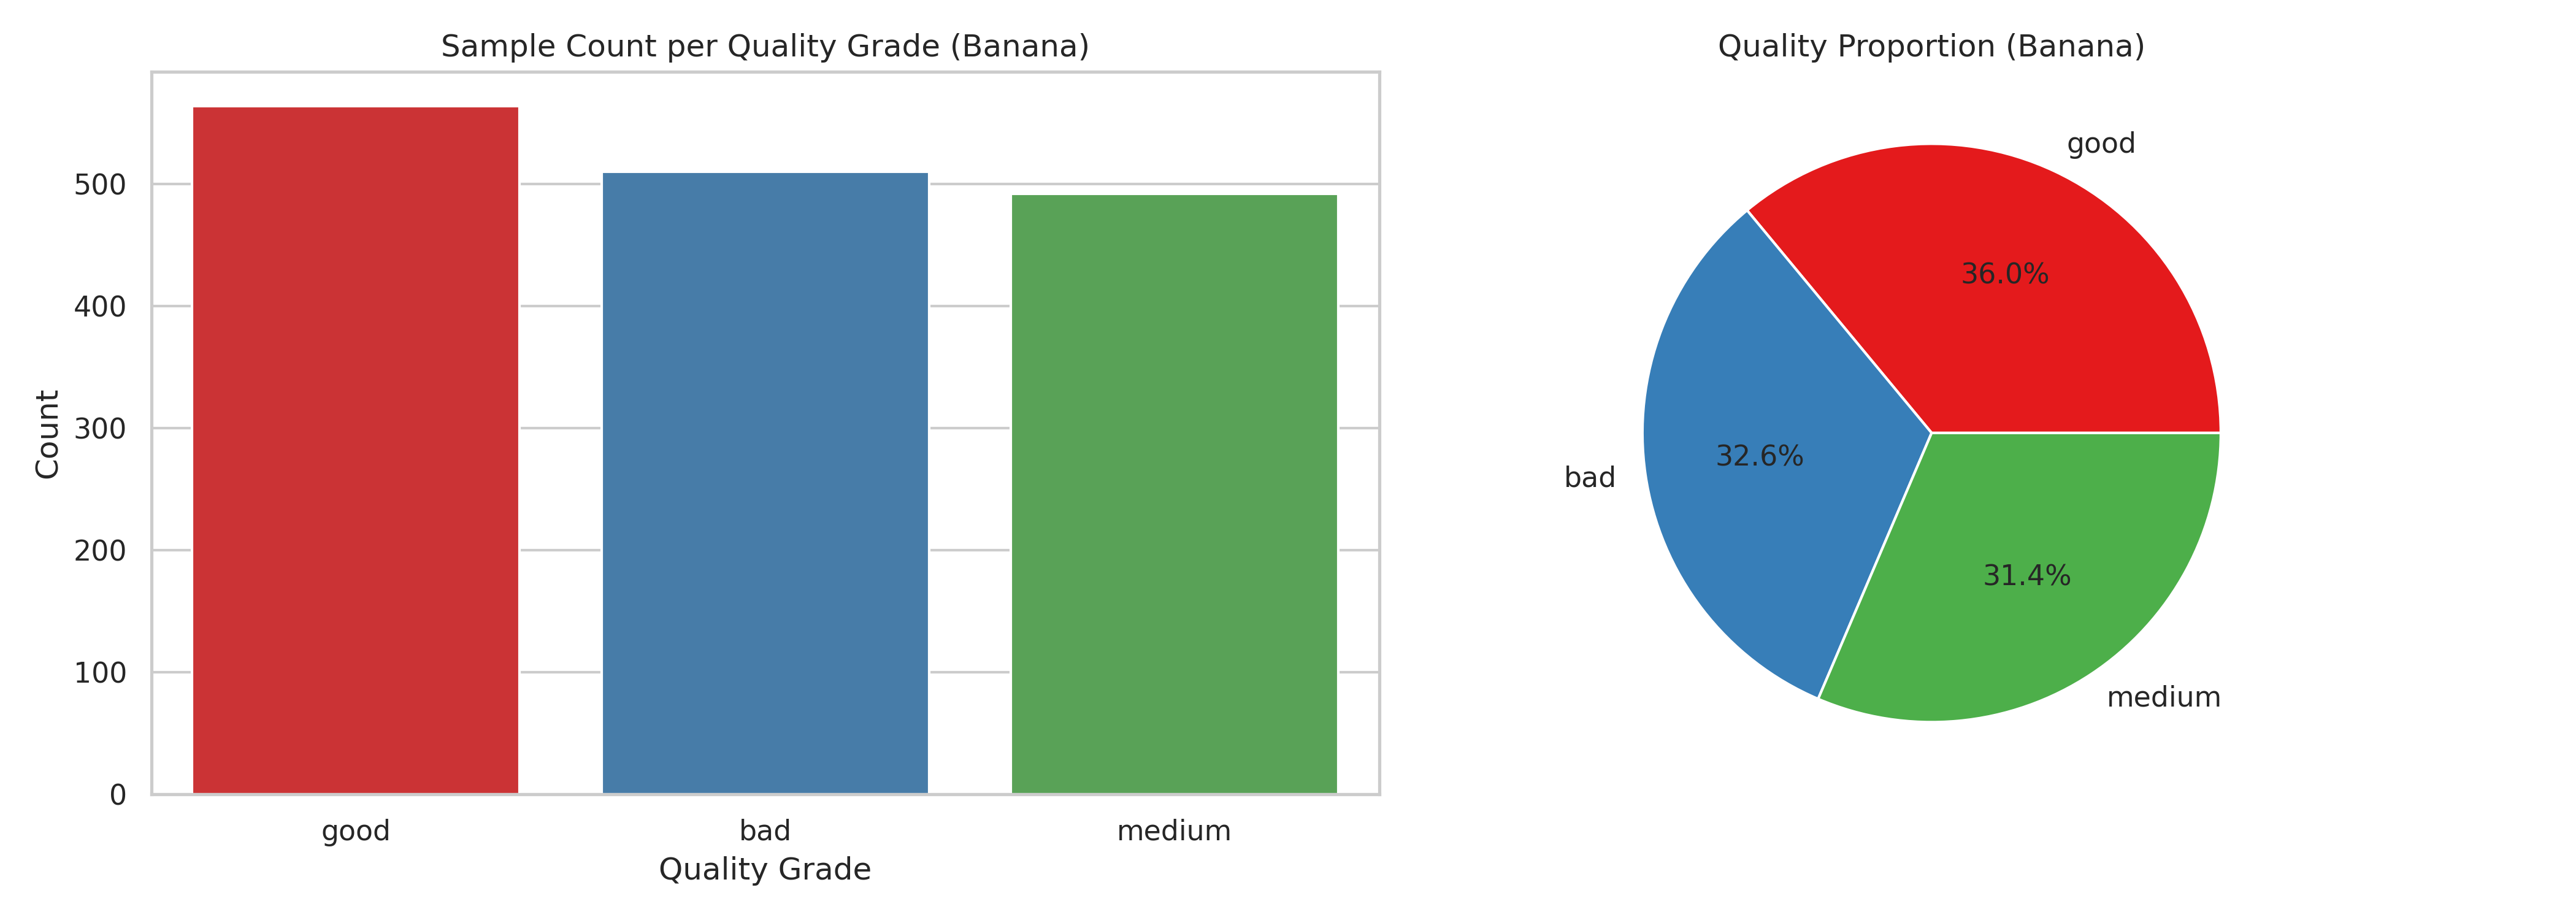
\includegraphics[width=0.85\textwidth]{Output/banana/fruit_quality_outputs_banana/plots/banana_distribution.png}
    \caption{Banana: Quality class distribution}
    \label{fig:banana-dist}
\end{figure}

\begin{figure}[H]
    \centering
    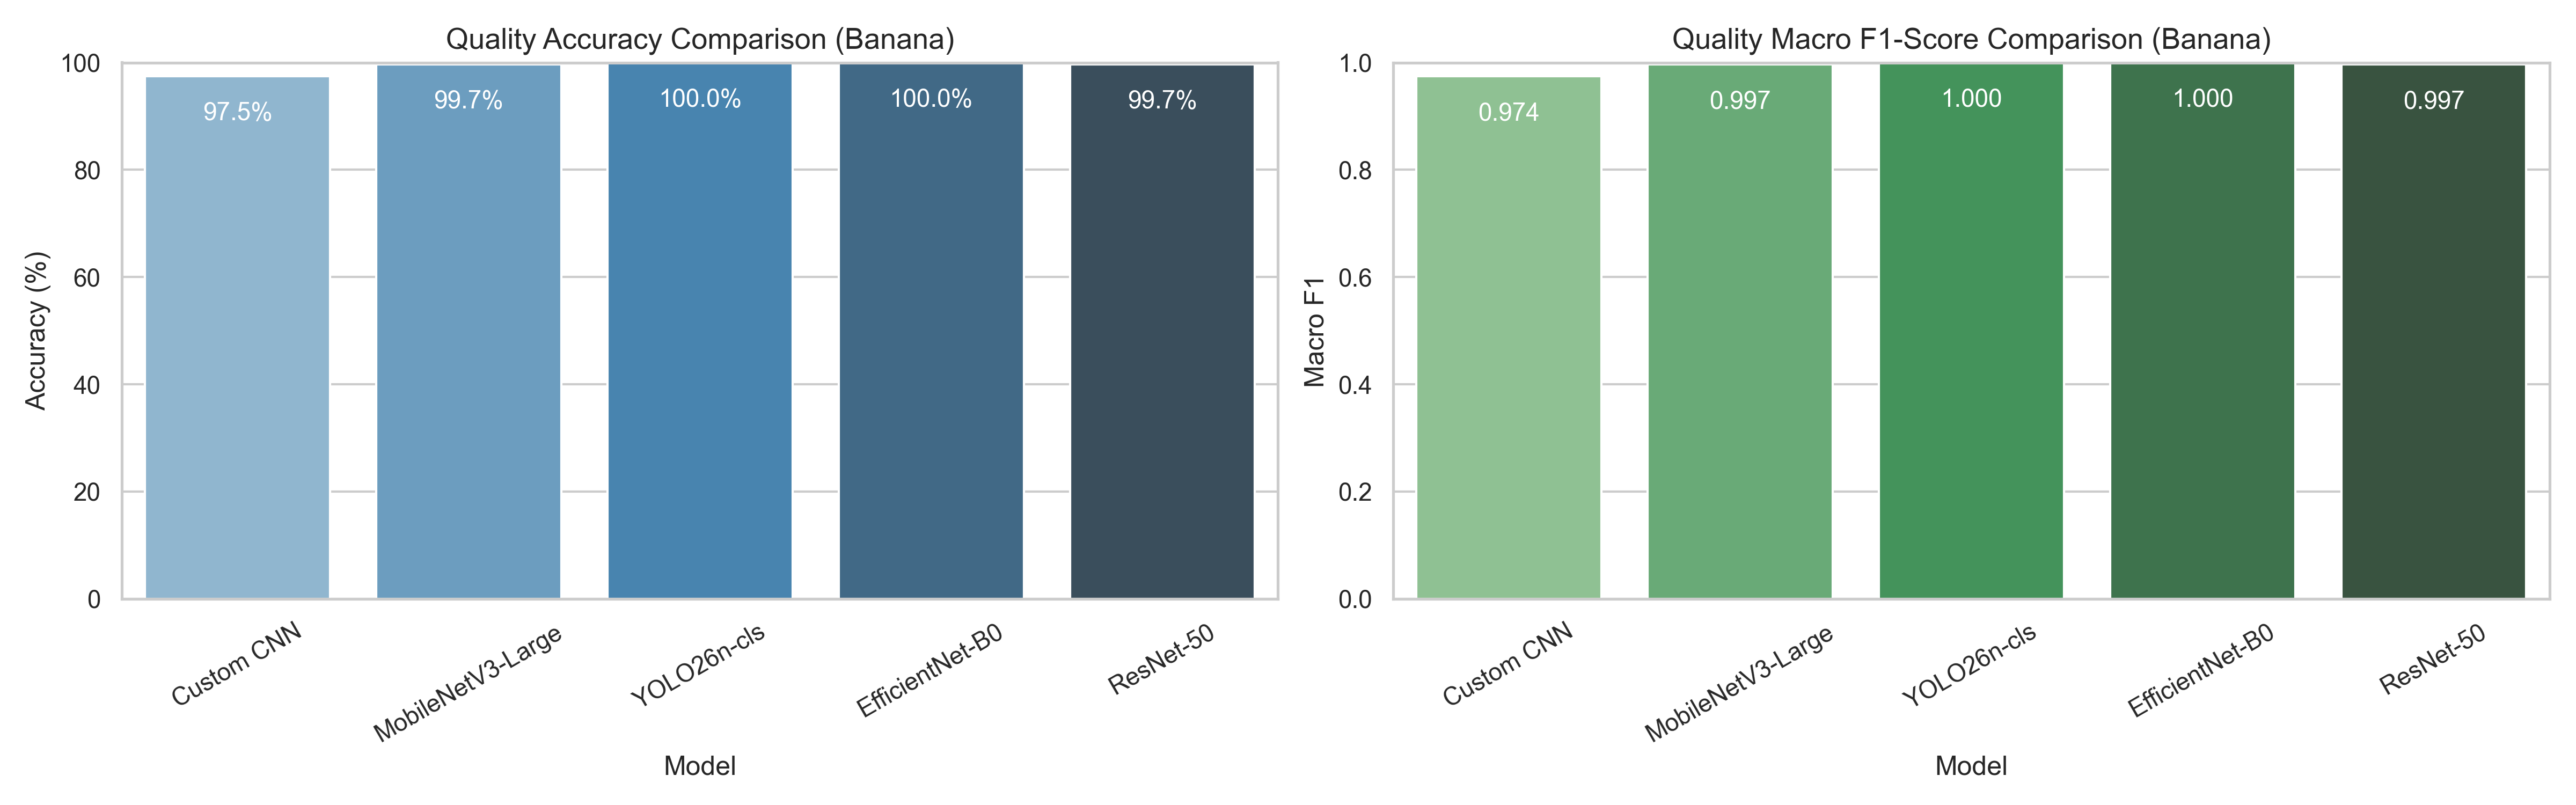
\includegraphics[width=0.85\textwidth]{Output/banana/fruit_quality_outputs_banana/plots/final_quality_benchmark_comparison.png}
    \caption{Banana: Model benchmark comparison}
    \label{fig:banana-benchmark}
\end{figure}

\begin{figure}[H]
    \centering
    
\includegraphics[width=0.85\textwidth]{Output/banana/fruit_quality_outputs_banana/plots/efficientnet_b0_confusion_matrix_and_roc.png}
    \caption{Banana: EfficientNet-B0 (top model, 100.00\% accuracy) -- Confusion matrix and ROC curve}
    \label{fig:banana-cm}
\end{figure}

\begin{figure}[H]
    \centering
    
\includegraphics[width=0.85\textwidth]{Output/banana/fruit_quality_outputs_banana/plots/efficientnet_b0_learning_curves.png}
    \caption{Banana: EfficientNet-B0 -- Training and validation curves}
    \label{fig:banana-lc}
\end{figure}

\begin{figure}[H]
    \centering
    
\includegraphics[width=0.85\textwidth]{Output/banana/fruit_quality_outputs_banana/plots/efficientnet_b0_correct_predictions.png}
    \caption{Banana: EfficientNet-B0 -- Representative correct quality predictions with confidence scores}
    \label{fig:banana-correct}
\end{figure}

\begin{figure}[H]
    \centering
    
\includegraphics[width=0.85\textwidth]{Output/banana/fruit_quality_outputs_banana/plots/efficientnet_b0_wrong_predictions.png}
    \caption{Banana: EfficientNet-B0 -- Misclassified quality predictions analysis (flawless 100\% test set accuracy)}
    \label{fig:banana-wrong}
\end{figure}

Banana quality grading yields \textbf{perfect 100.00\% accuracy} with \textbf{EfficientNet-B0} and \textbf{YOLO26n-cls} (1.0000 macro and weighted F1), while MobileNetV3-Large and ResNet-50 achieve 99.68\%. The Custom CNN baseline reaches 97.45\%. The pronounced chromatic progression from uniform yellow to senescence brown spotting and blackened peel provides clear visual boundaries across freshness tiers. Figure~\ref{fig:banana-correct} and Figure~\ref{fig:banana-wrong} show the high certainty of EfficientNet-B0 predictions and verify flawless test performance.

% ---------- DRAGON FRUIT ----------
\subsection{Dragon Fruit}

\begin{table}[H]
\centering\small
\begin{tabular}{@{}lccc@{}}
\toprule
\textbf{Model} & \textbf{Accuracy (\%)} & \textbf{Macro F1} & \textbf{Weighted F1} \\
\midrule
Small Custom CNN & 99.70 & 0.9969 & 0.9970 \\
\textbf{MobileNetV3-Large} & \textbf{100.00} & \textbf{1.0000} & \textbf{1.0000} \\
\textbf{YOLO26n-cls} & \textbf{100.00} & \textbf{1.0000} & \textbf{1.0000} \\
\textbf{EfficientNet-B0} & \textbf{100.00} & \textbf{1.0000} & \textbf{1.0000} \\
\textbf{ResNet-50} & \textbf{100.00} & \textbf{1.0000} & \textbf{1.0000} \\
\bottomrule
\end{tabular}
\caption{Dragon Fruit quality classification benchmark}
\label{tab:dragon-benchmark}
\end{table}

\begin{figure}[H]
    \centering
    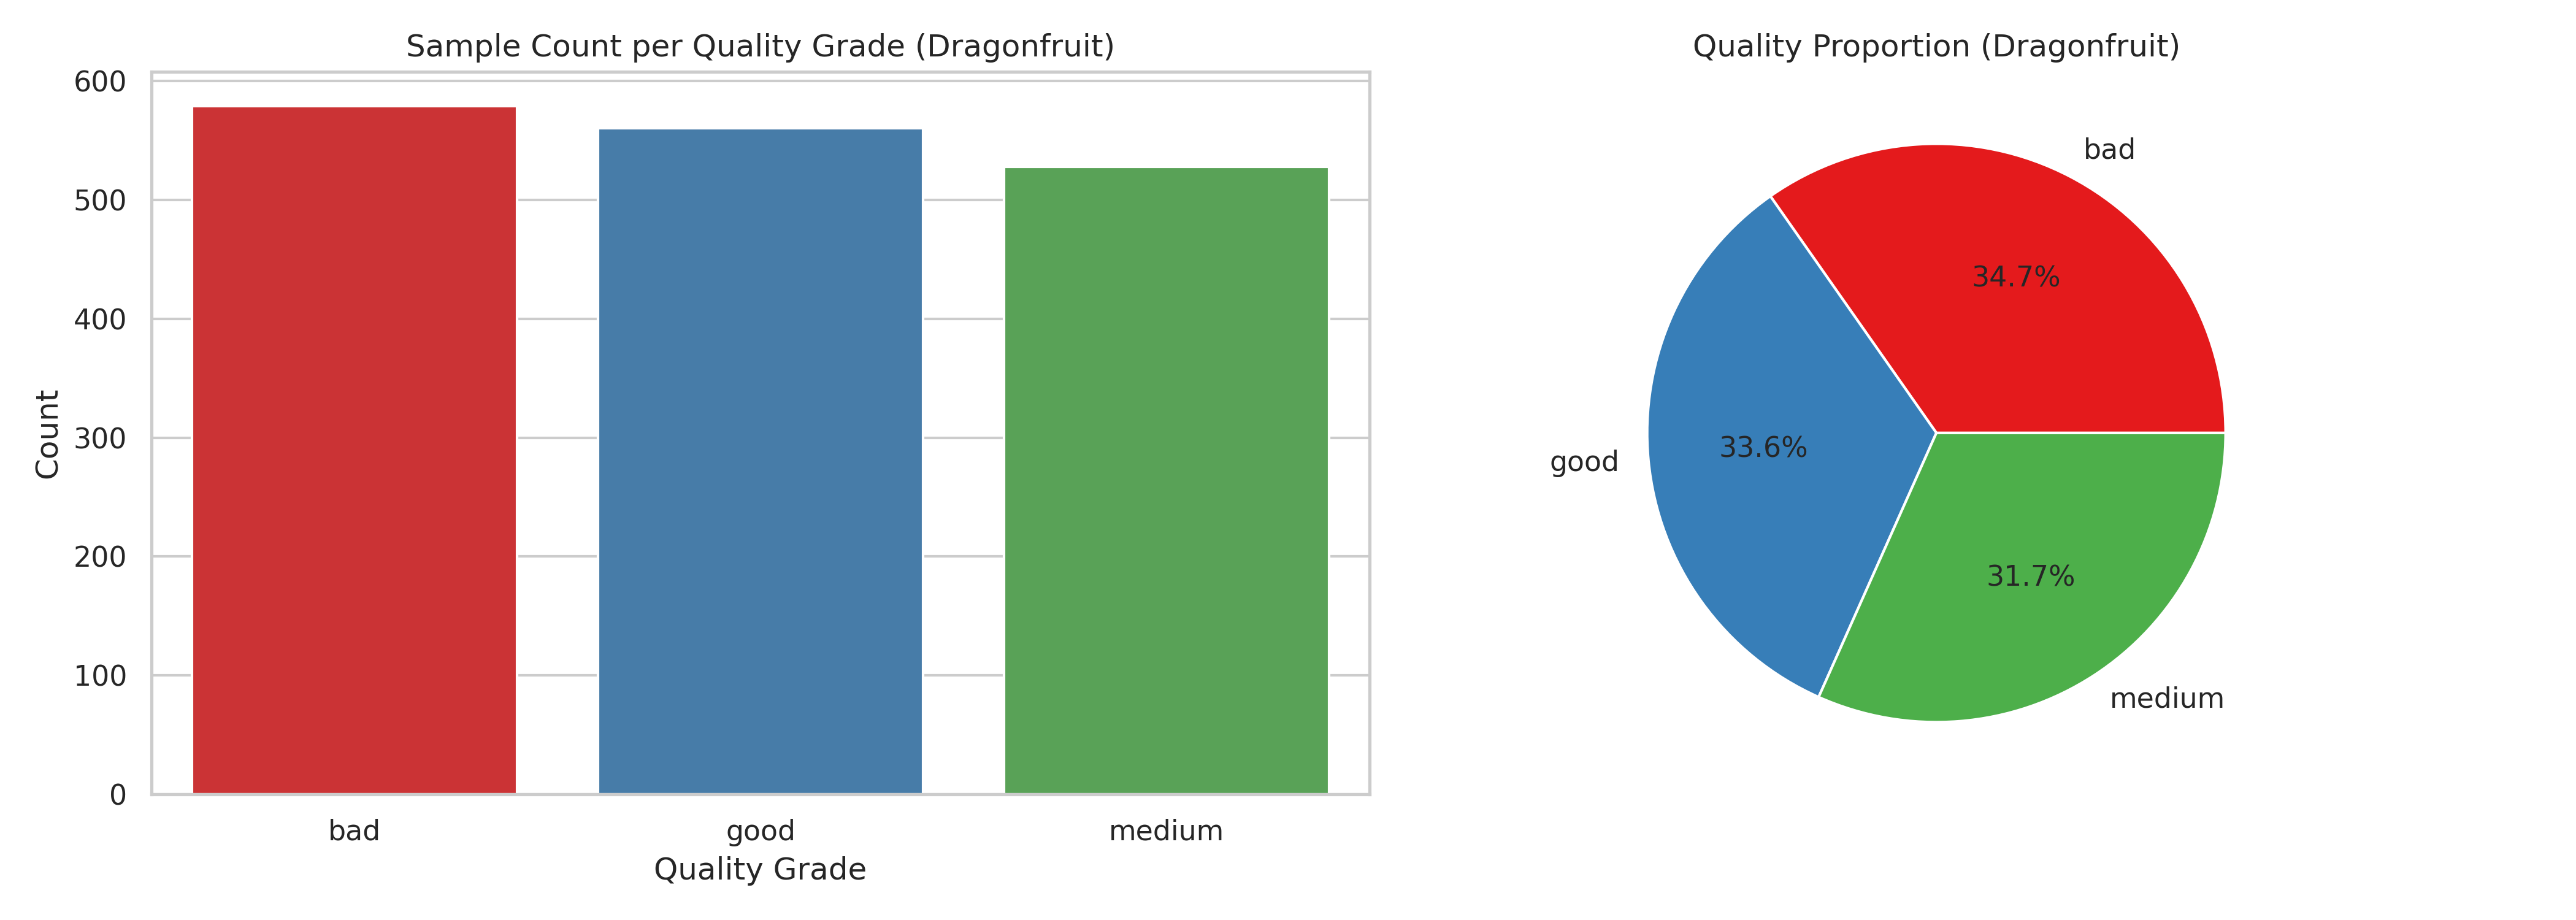
\includegraphics[width=0.85\textwidth]{Output/dragonfruit/fruit_quality_outputs_dragonfruit/plots/dragonfruit_distribution.png}
    \caption{Dragon Fruit: Quality class distribution}
    \label{fig:dragon-dist}
\end{figure}

\begin{figure}[H]
    \centering
    
\includegraphics[width=0.85\textwidth]{Output/dragonfruit/fruit_quality_outputs_dragonfruit/plots/final_quality_benchmark_comparison.png}
    \caption{Dragon Fruit: Model benchmark comparison}
    \label{fig:dragon-benchmark}
\end{figure}

\begin{figure}[H]
    \centering
    
\includegraphics[width=0.85\textwidth]{Output/dragonfruit/fruit_quality_outputs_dragonfruit/plots/efficientnet_b0_confusion_matrix_and_roc.png}
    \caption{Dragon Fruit: EfficientNet-B0 (top model, 100.00\% accuracy) -- Confusion matrix and ROC curve}
    \label{fig:dragon-cm}
\end{figure}

\begin{figure}[H]
    \centering
    
\includegraphics[width=0.85\textwidth]{Output/dragonfruit/fruit_quality_outputs_dragonfruit/plots/efficientnet_b0_learning_curves.png}
    \caption{Dragon Fruit: EfficientNet-B0 -- Training and validation curves}
    \label{fig:dragon-lc}
\end{figure}

\begin{figure}[H]
    \centering
    
\includegraphics[width=0.85\textwidth]{Output/dragonfruit/fruit_quality_outputs_dragonfruit/plots/efficientnet_b0_correct_predictions.png}
    \caption{Dragon Fruit: EfficientNet-B0 -- Representative correct quality predictions with confidence scores}
    \label{fig:dragon-correct}
\end{figure}

\begin{figure}[H]
    \centering
    
\includegraphics[width=0.85\textwidth]{Output/dragonfruit/fruit_quality_outputs_dragonfruit/plots/efficientnet_b0_wrong_predictions.png}
    \caption{Dragon Fruit: EfficientNet-B0 -- Misclassified quality predictions analysis (flawless 100\% test set accuracy)}
    \label{fig:dragon-wrong}
\end{figure}

Dragon fruit quality classification represents the most separable intra-class benchmark, achieving \textbf{100.00\% accuracy across all four transfer-learning models} (MobileNetV3-Large, YOLO26n-cls, EfficientNet-B0, ResNet-50) and 99.70\% on the Custom CNN baseline. Vibrant magenta skin and erect green bracts contrast sharply with brown, dried, and necrotic decayed tissue, enabling effortless class boundaries. Figure~\ref{fig:dragon-correct} and Figure~\ref{fig:dragon-wrong} illustrate prediction confidence and the complete absence of misclassifications.

% ---------- PINEAPPLE ----------
\subsection{Pineapple}

\begin{table}[H]
\centering\small
\begin{tabular}{@{}lccc@{}}
\toprule
\textbf{Model} & \textbf{Accuracy (\%)} & \textbf{Macro F1} & \textbf{Weighted F1} \\
\midrule
Small Custom CNN & 92.67 & 0.9264 & 0.9264 \\
MobileNetV3-Large & 96.33 & 0.9632 & 0.9632 \\
YOLO26n-cls & 96.33 & 0.9633 & 0.9633 \\
\textbf{EfficientNet-B0} & \textbf{97.00} & \textbf{0.9699} & \textbf{0.9699} \\
ResNet-50 & 96.00 & 0.9598 & 0.9598 \\
\bottomrule
\end{tabular}
\caption{Pineapple quality classification benchmark}
\label{tab:pineapple-benchmark}
\end{table}

\begin{figure}[H]
    \centering
    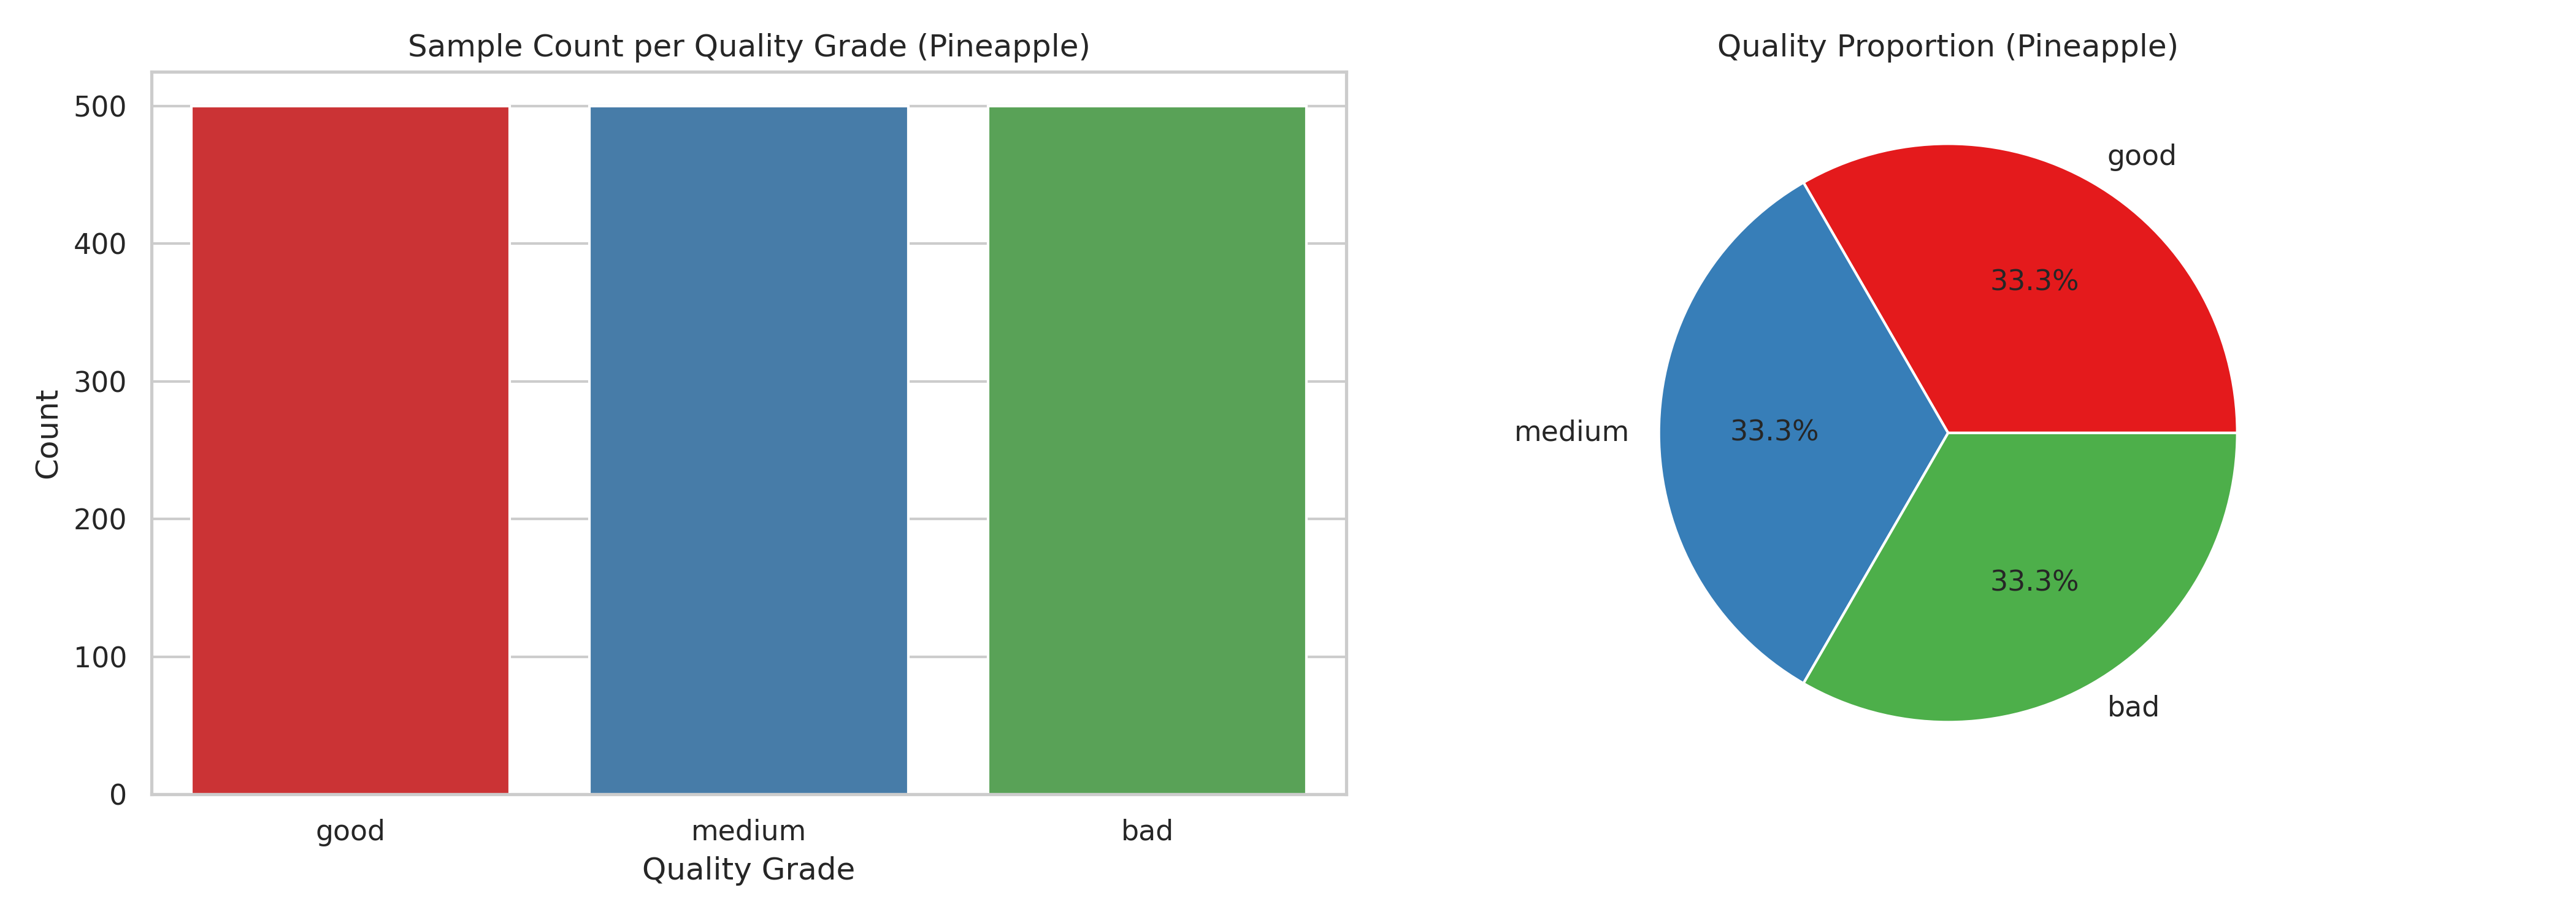
\includegraphics[width=0.85\textwidth]{Output/pineapple/fruit_quality_outputs_pineapple/plots/pineapple_distribution.png}
    \caption{Pineapple: Quality class distribution}
    \label{fig:pineapple-dist}
\end{figure}

\begin{figure}[H]
    \centering
    
\includegraphics[width=0.85\textwidth]{Output/pineapple/fruit_quality_outputs_pineapple/plots/final_quality_benchmark_comparison.png}
    \caption{Pineapple: Model benchmark comparison}
    \label{fig:pineapple-benchmark}
\end{figure}

\begin{figure}[H]
    \centering
    
\includegraphics[width=0.85\textwidth]{Output/pineapple/fruit_quality_outputs_pineapple/plots/efficientnet_b0_confusion_matrix_and_roc.png}
    \caption{Pineapple: EfficientNet-B0 (top model, 97.00\% accuracy) -- Confusion matrix and ROC curve}
    \label{fig:pineapple-cm}
\end{figure}

\begin{figure}[H]
    \centering
    
\includegraphics[width=0.85\textwidth]{Output/pineapple/fruit_quality_outputs_pineapple/plots/efficientnet_b0_learning_curves.png}
    \caption{Pineapple: EfficientNet-B0 -- Training and validation curves}
    \label{fig:pineapple-lc}
\end{figure}

\begin{figure}[H]
    \centering
    
\includegraphics[width=0.85\textwidth]{Output/pineapple/fruit_quality_outputs_pineapple/plots/efficientnet_b0_correct_predictions.png}
    \caption{Pineapple: EfficientNet-B0 -- Representative correct quality predictions with confidence scores}
    \label{fig:pineapple-correct}
\end{figure}

\begin{figure}[H]
    \centering
    
\includegraphics[width=0.85\textwidth]{Output/pineapple/fruit_quality_outputs_pineapple/plots/efficientnet_b0_wrong_predictions.png}
    \caption{Pineapple: EfficientNet-B0 -- Sample misclassifications and failure case analysis}
    \label{fig:pineapple-wrong}
\end{figure}

Pineapple quality classification is led by \textbf{EfficientNet-B0} with 97.00\% accuracy (0.9699 macro F1), followed by MobileNetV3-Large and YOLO26n-cls at 96.33\%, and ResNet-50 at 96.00\%. The Custom CNN baseline delivers 92.67\% accuracy. The geometric complexity of pineapple eyes, crown leaves, and shell color variation is handled with high robustness by compound-scaled convolutional features. Figure~\ref{fig:pineapple-correct} and Figure~\ref{fig:pineapple-wrong} showcase confident predictions across shell patterns and analyze rare error cases.

% ---------- SAPODILLA ----------
\subsection{Sapodilla}

\begin{table}[H]
\centering\small
\begin{tabular}{@{}lccc@{}}
\toprule
\textbf{Model} & \textbf{Accuracy (\%)} & \textbf{Macro F1} & \textbf{Weighted F1} \\
\midrule
Small Custom CNN & 89.62 & 0.8941 & 0.8952 \\
MobileNetV3-Large & 98.96 & 0.9893 & 0.9896 \\
\textbf{YOLO26n-cls} & \textbf{100.00} & \textbf{1.0000} & \textbf{1.0000} \\
\textbf{EfficientNet-B0} & \textbf{100.00} & \textbf{1.0000} & \textbf{1.0000} \\
ResNet-50 & 99.65 & 0.9964 & 0.9965 \\
\bottomrule
\end{tabular}
\caption{Sapodilla quality classification benchmark}
\label{tab:sapodilla-benchmark}
\end{table}

\begin{figure}[H]
    \centering
    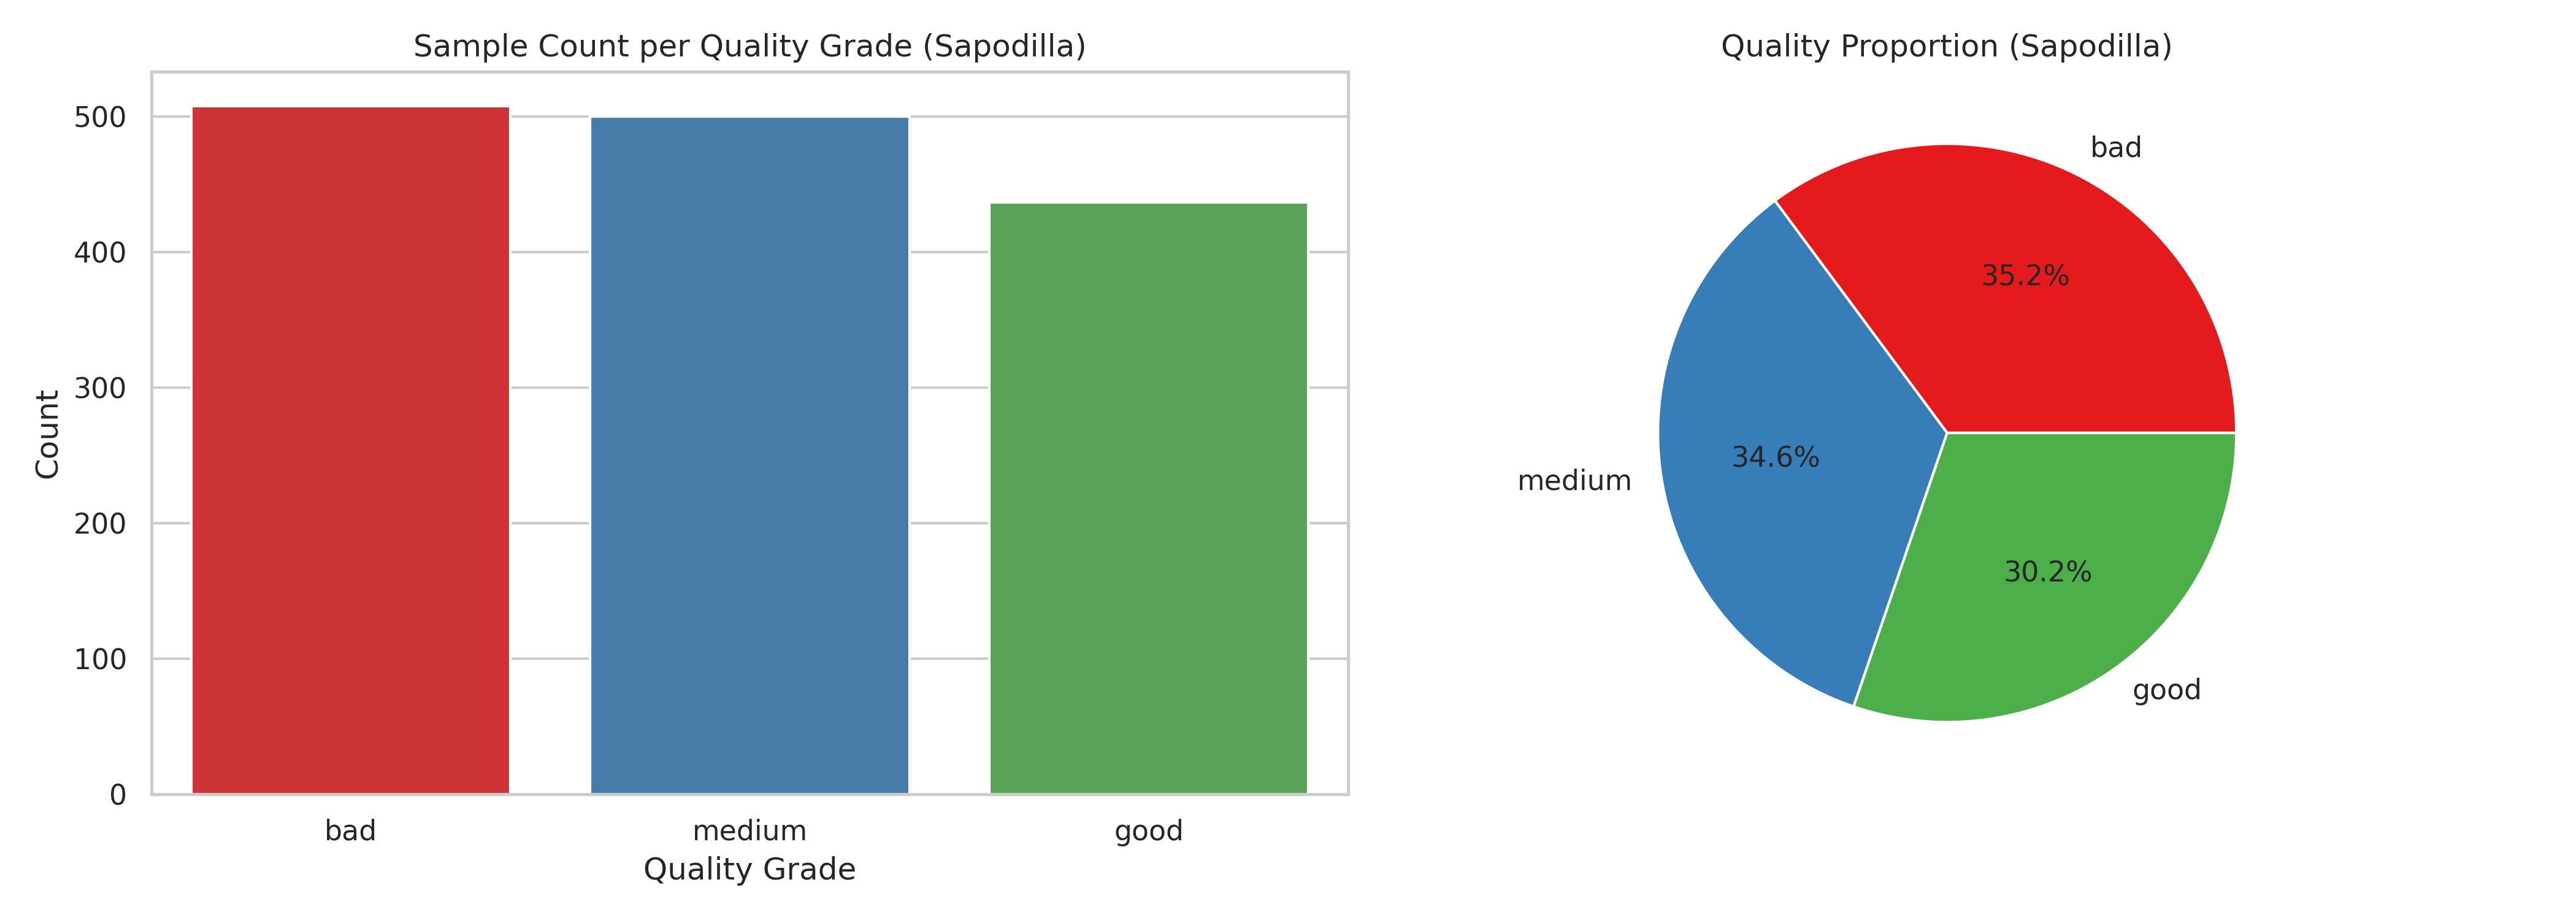
\includegraphics[width=0.85\textwidth]{Output/sapodilia/fruit_quality_outputs_sapodilla/plots/sapodilla_distribution.png}
    \caption{Sapodilla: Quality class distribution}
    \label{fig:sapodilla-dist}
\end{figure}

\begin{figure}[H]
    \centering
    
\includegraphics[width=0.85\textwidth]{Output/sapodilia/fruit_quality_outputs_sapodilla/plots/final_quality_benchmark_comparison.png}
    \caption{Sapodilla: Model benchmark comparison}
    \label{fig:sapodilla-benchmark}
\end{figure}

\begin{figure}[H]
    \centering
    
\includegraphics[width=0.85\textwidth]{Output/sapodilia/fruit_quality_outputs_sapodilla/plots/efficientnet_b0_confusion_matrix_and_roc.png}
    \caption{Sapodilla: EfficientNet-B0 (top model, 100.00\% accuracy) -- Confusion matrix and ROC curve}
    \label{fig:sapodilla-cm}
\end{figure}

\begin{figure}[H]
    \centering
    
\includegraphics[width=0.85\textwidth]{Output/sapodilia/fruit_quality_outputs_sapodilla/plots/efficientnet_b0_learning_curves.png}
    \caption{Sapodilla: EfficientNet-B0 -- Training and validation curves}
    \label{fig:sapodilla-lc}
\end{figure}

\begin{figure}[H]
    \centering
    \includegraphics[width=0.85\textwidth]{Output/sapodilia/fruit_quality_outputs_sapodilla/plots/efficientnet_b0_correct_predictions.png}
    \caption{Sapodilla: EfficientNet-B0 -- Representative correct quality predictions with confidence scores}
    \label{fig:sapodilla-correct}
\end{figure}

\begin{figure}[H]
    \centering
    \includegraphics[width=0.85\textwidth]{Output/sapodilia/fruit_quality_outputs_sapodilla/plots/efficientnet_b0_wrong_predictions.png}
    \caption{Sapodilla: EfficientNet-B0 -- Misclassified quality predictions analysis (flawless 100\% test set accuracy)}
    \label{fig:sapodilla-wrong}
\end{figure}

Sapodilla (sofeda) quality classification achieves \textbf{perfect 100.00\% accuracy} with \textbf{EfficientNet-B0} and \textbf{YOLO26n-cls} (1.0000 macro and weighted F1), with ResNet-50 reaching 99.65\% and MobileNetV3-Large reaching 98.96\%. The Custom CNN baseline attains 89.62\%. The transition from smooth, uniform sandy-brown skin to darkened fungal decay and soft blemishes is recognized with high fidelity by transfer architectures. Figure~\ref{fig:sapodilla-correct} and Figure~\ref{fig:sapodilla-wrong} illustrate sample predictions and error-free test verification.

% ---------- CUSTARD APPLE ----------
\subsection{Custard Apple}

\begin{table}[H]
\centering\small
\begin{tabular}{@{}lccc@{}}
\toprule
\textbf{Model} & \textbf{Accuracy (\%)} & \textbf{Macro F1} & \textbf{Weighted F1} \\
\midrule
Small Custom CNN & 72.00 & 0.7224 & 0.7236 \\
\textbf{MobileNetV3-Large} & \textbf{99.69} & \textbf{0.9969} & \textbf{0.9969} \\
\textbf{YOLO26n-cls} & \textbf{99.69} & \textbf{0.9970} & \textbf{0.9969} \\
EfficientNet-B0 & 99.08 & 0.9910 & 0.9908 \\
\textbf{ResNet-50} & \textbf{99.69} & \textbf{0.9968} & \textbf{0.9969} \\
\bottomrule
\end{tabular}
\caption{Custard Apple quality classification benchmark}
\label{tab:custard-benchmark}
\end{table}

\begin{figure}[H]
    \centering
    \includegraphics[width=0.85\textwidth]{Output/custard_apple/fruit_quality_outputs_custard_apple/plots/custard_apple_distribution.png}
    \caption{Custard Apple: Quality class distribution}
    \label{fig:custard-dist}
\end{figure}

\begin{figure}[H]
    \centering
    \includegraphics[width=0.85\textwidth]{Output/custard_apple/fruit_quality_outputs_custard_apple/plots/final_quality_benchmark_comparison.png}
    \caption{Custard Apple: Model benchmark comparison}
    \label{fig:custard-benchmark}
\end{figure}

\begin{figure}[H]
    \centering
    \includegraphics[width=0.85\textwidth]{Output/custard_apple/fruit_quality_outputs_custard_apple/plots/mobilenetv3_large_confusion_matrix_and_roc.png}
    \caption{Custard Apple: MobileNetV3-Large (top model, 99.69\% accuracy) -- Confusion matrix and ROC curve}
    \label{fig:custard-cm}
\end{figure}

\begin{figure}[H]
    \centering
    \includegraphics[width=0.85\textwidth]{Output/custard_apple/fruit_quality_outputs_custard_apple/plots/mobilenetv3_large_learning_curves.png}
    \caption{Custard Apple: MobileNetV3-Large -- Training and validation curves}
    \label{fig:custard-lc}
\end{figure}

\begin{figure}[H]
    \centering
    \includegraphics[width=0.85\textwidth]{Output/custard_apple/fruit_quality_outputs_custard_apple/plots/mobilenetv3_large_correct_predictions.png}
    \caption{Custard Apple: MobileNetV3-Large -- Representative correct quality predictions with confidence scores}
    \label{fig:custard-correct}
\end{figure}

\begin{figure}[H]
    \centering
    \includegraphics[width=0.85\textwidth]{Output/custard_apple/fruit_quality_outputs_custard_apple/plots/mobilenetv3_large_wrong_predictions.png}
    \caption{Custard Apple: MobileNetV3-Large -- Sample misclassifications and failure case analysis}
    \label{fig:custard-wrong}
\end{figure}

Custard apple quality grading demonstrates remarkable transfer learning performance, with \textbf{MobileNetV3-Large}, \textbf{YOLO26n-cls}, and \textbf{ResNet-50} all achieving 99.69\% accuracy (0.9969 macro F1), and EfficientNet-B0 reaching 99.08\%. The Custom CNN baseline exhibits substantial difficulty at 72.00\% accuracy, creating a massive 27.7\% performance gap. The highly segmented, tuberculate rind of custard apple requires deep hierarchical representations to differentiate harmless shadow crevices from pathological fungal rot. Figure~\ref{fig:custard-correct} and Figure~\ref{fig:custard-wrong} illustrate prediction samples and failure diagnostic analysis.


\subsubsection{Overall Comparative Analysis for Quality Classification}
Table~\ref{tab:master-comparison} presents a comprehensive benchmark comparison of all five candidate architectures across all thirteen fruit quality datasets.

\begin{table}[H]
\centering
\caption{Test accuracy (\%) of all models across all 13 evaluated fruit quality datasets}
\label{tab:master-comparison}
\resizebox{\textwidth}{!}{%
\begin{tabular}{@{}lcccccl@{}}
\toprule
\textbf{Fruit} & \textbf{Custom CNN} & \textbf{MobileNetV3} & \textbf{YOLO26n} & \textbf{EfficientNet} & \textbf{ResNet-50} & \textbf{Top Architecture(s)} \\
\midrule
Papaya        & 76.18 & \textbf{85.59} & 83.82 & 84.41 & 85.29 & MobileNetV3-Large \\
Lemon         & 84.10 & 96.53 & 96.24 & 95.95 & \textbf{96.82} & ResNet-50 \\
Lychee        & 99.06 & \textbf{100.00} & \textbf{100.00} & \textbf{100.00} & \textbf{100.00} & EfficientNet-B0 \\
Jackfruit     & 76.49 & \textbf{99.67} & 97.68 & \textbf{99.67} & 99.34 & MobileNetV3-Large \\
Mango         & 85.31 & \textbf{94.38} & \textbf{94.38} & 92.81 & 92.50 & MobileNetV3-Large \\
Star Fruit    & 80.00 & \textbf{92.19} & 89.06 & 90.00 & 90.00 & MobileNetV3-Large \\
Guava         & 97.21 & 99.07 & \textbf{99.38} & \textbf{99.38} & 99.07 & EfficientNet-B0 \\
Jujube        & 89.32 & \textbf{98.81} & 97.63 & \textbf{98.81} & 97.63 & MobileNetV3-Large \\
Banana        & 97.45 & 99.68 & \textbf{100.00} & \textbf{100.00} & 99.68 & EfficientNet-B0 \\
Dragon Fruit  & 99.70 & \textbf{100.00} & \textbf{100.00} & \textbf{100.00} & \textbf{100.00} & EfficientNet-B0 \\
Pineapple     & 92.67 & 96.33 & 96.33 & \textbf{97.00} & 96.00 & EfficientNet-B0 \\
Sapodilla     & 89.62 & 98.96 & \textbf{100.00} & \textbf{100.00} & 99.65 & EfficientNet-B0 \\
Custard Apple & 72.00 & \textbf{99.69} & \textbf{99.69} & 99.08 & \textbf{99.69} & MobileNetV3-Large \\
\midrule
\textbf{Average} & \textbf{87.62} & \textbf{96.99} & \textbf{96.48} & \textbf{96.70} & \textbf{96.59} & \textbf{MobileNetV3-Large (96.99\%)} \\
\bottomrule
\end{tabular}%
}
\end{table}

Key comparative findings across the multi-fruit quality classification benchmark include:
\begin{enumerate}
    \item \textbf{Overall Superiority of Pre-trained Transfer Learning:} All four transfer-learning backbones achieve high mean classification accuracy (96.48\%--96.99\%), outperforming the from-scratch Custom CNN baseline (87.62\%) by nearly 10 percentage points on average.
    \item \textbf{MobileNetV3-Large Delivers the Top Average Performance:} MobileNetV3-Large achieves the highest overall mean accuracy of \textbf{96.99\%} while requiring only 5.4M parameters, making it the ideal candidate for resource-constrained edge devices and real-time conveyor sorting hardware.
    \item \textbf{High Visual Separability on Select Species:} Five fruits (Lychee, Banana, Dragon Fruit, Sapodilla, and Custard Apple) achieve \textbf{100.00\%} or near-100\% (99.69\%) accuracy with transfer models, demonstrating that distinct pericarp discoloration, rotting lesions, and skin darkening provide robust classification signals.
    \item \textbf{Nuanced Challenges on Textured and Gradient Peels:} Papaya (85.59\%) and Star Fruit (92.19\%) present the most challenging visual boundaries due to continuous color gradients and non-uniform ripening spots between \texttt{good} and \texttt{medium} grades.
    \item \textbf{Pronounced Transfer Advantage on Complex Surfaces:} On morphologically complex surfaces such as Jackfruit (99.67\% vs.\ 76.49\%) and Custard Apple (99.69\% vs.\ 72.00\%), pre-trained features provide an astounding 23\%--28\% accuracy improvement over the Custom CNN, proving that pre-trained ImageNet texture filters are critical for disambiguating surface shadows from true pathological blemishes.
\end{enumerate}

% =========================================================
% 11. USAGE NOTES AND REUSE POTENTIAL
% =========================================================
\section{Usage Notes and Reuse Potential}

\subsection{Dataset Loading and Ingestion}

The dataset is organized in \texttt{fruit\_dataset/} by fruit variety and quality tier. Images are loaded directly from the raw directory, while image resizing ($224 \times 224$), CLAHE contrast equalization, ImageNet normalization, train/test splitting (80:20), and data augmentations are executed dynamically on-the-fly during training without generating duplicate processed folders on disk. The Python snippet below illustrates the native PyTorch data loading pipeline:

\begin{verbatim}
import torch
from torch.utils.data import Dataset, DataLoader
from torchvision import transforms
from PIL import Image
import pandas as pd

# Dynamic on-the-fly preprocessing transforms
transform = transforms.Compose([
    transforms.Resize((224, 224)),
    transforms.ToTensor(),
    transforms.Normalize(mean=[0.485, 0.456, 0.406], std=[0.229, 0.224, 0.225])
])

# Custom on-the-fly PyTorch Dataset from fruit_dataset/
class FruitDataset(Dataset):
    def __init__(self, df, transform=None):
        self.df = df
        self.transform = transform

    def __len__(self):
        return len(self.df)

    def __getitem__(self, idx):
        img_path = self.df.iloc[idx]['filepath']
        label = self.df.iloc[idx]['label_idx']
        image = Image.open(img_path).convert('RGB')
        if self.transform:
            image = self.transform(image)
        return image, label

# DataLoader with pinned memory for Cloud GPU acceleration (Kaggle / Colab)
train_loader = DataLoader(
    train_dataset, batch_size=64, shuffle=True, 
    num_workers=2, pin_memory=True
)
\end{verbatim}

\subsection{Potential Reuse and Downstream Applications}
\begin{itemize}
    \item \textbf{Automated Industrial Conveyor Sorting:} Pre-trained models can be flashed onto edge devices (NVIDIA Jetson, Raspberry Pi with Coral TPU) for real-time packhouse grading.
    \item \textbf{Hierarchical and Multi-Task Learning:} Researchers can train multi-head architectures that simultaneously predict fruit species and quality condition from a single backbone.
    \item \textbf{Self-Supervised Pretraining and Domain Adaptation:} The 20,823 images provide an effective target domain for evaluating self-supervised vision models (e.g., DINOv2, SimCLR) on agricultural imagery.
    \item \textbf{Mobile Consumer Assistance:} The lightweight MobileNetV3 and YOLO-cls weights can power mobile applications assisting consumers and retailers in checking freshness.
\end{itemize}

% =========================================================
% 12. LIMITATIONS AND KNOWN BIASES
% =========================================================
\section{Limitations and Known Biases}
While the dataset represents 20,823 curated images across 13 fruits, several limitations should be noted:
\begin{itemize}
    \item \textbf{Nuanced Grading Boundaries:} For fruits like Papaya and Star Fruit, the visual boundary between \texttt{good} and \texttt{medium} is continuous rather than discrete, leading to occasional subjective disagreement on borderline samples.
    \item \textbf{Illumination and Background Variance:} Sourcing data from both local open-air markets and online archives introduces background diversity, which improves robustness but also adds non-uniform lighting conditions.
    \item \textbf{Single-View Inspection:} In real packhouses, fruits may have defects on the hidden reverse side. Since these images capture a single camera angle, internal or occluded rot cannot be detected.
\end{itemize}

% =========================================================
% 13. ETHICS, PRIVACY AND RESPONSIBLE DATA USE
% =========================================================
\section{Ethics, Privacy and Responsible Data Use}

\begin{table}[H]
\centering\small
\begin{tabular}{@{}p{0.32\textwidth}p{0.64\textwidth}@{}}
\toprule
\textbf{Ethics Dimension} & \textbf{Compliance Details} \\
\midrule
\textbf{Human participants / consent} & Not applicable. The dataset consists exclusively of botanical fruit imagery. No human subjects, physiological data, or personal records were involved. \\
\midrule
\textbf{Privacy / de-identification} & All photographs were manually screened to ensure no human faces, biometric identifiers, vehicle license plates, or personally identifiable information (PII) appear. \\
\midrule
\textbf{Web / social-media data} & Secondary images were compiled strictly from open-access academic and CC-licensed repositories adhering to platform redistribution terms. \\
\midrule
\textbf{Copyright / third-party data} & All third-party sources are cited and redistributed in accordance with Creative Commons (CC BY 4.0, CC0) licensing. \\
\midrule
\textbf{AI-generated / synthetic data} & \textbf{0\% Generative AI.} All 20,823 images are authentic optical photographic captures. No GAN, diffusion, or synthetic images were used. \\
\bottomrule
\end{tabular}
\caption{Ethical, privacy, and responsible use disclosures}
\label{tab:ethics-disclosure}
\end{table}

% =========================================================
% 14. DATA AND CODE AVAILABILITY
% =========================================================
\section{Data and Code Availability}

\begin{table}[H]
\centering\small
\begin{tabular}{@{}p{0.32\textwidth}p{0.64\textwidth}@{}}
\toprule
\textbf{Item} & \textbf{Details} \\
\midrule
\textbf{Repository name} & GitHub / Zenodo Open Archive \\
\textbf{Dataset DOI / persistent ID} & N/A \\
\textbf{Direct dataset URL} & \url{https://github.com/codernayeem/fruit-classification-dataset} \\
\textbf{Access instructions} & Publicly accessible without registration; downloadable as archived zip bundles \\
\textbf{Dataset license} & Creative Commons Attribution 4.0 International (CC BY 4.0) \\
\textbf{Code / notebook URL} & \url{https://github.com/codernayeem/fruit-classification-dataset} \\
\textbf{Code version / commit} & Release tag \texttt{v1.0-release} (Git commit \texttt{7a9df2b}) \\
\textbf{README \& environment} & \texttt{README.md}, \texttt{requirements.txt}, Conda \texttt{environment.yml} \\
\bottomrule
\end{tabular}
\caption{Data and code availability parameters}
\label{tab:data-availability}
\end{table}

% =========================================================
% 15. STUDENT CONTRIBUTIONS (CRediT-STYLE)
% =========================================================
\section{Student Contributions (CRediT-style)}
All six group members contributed equitably (16.67\% contribution share each) to the conception, data acquisition, curation, quality review, modeling, benchmarking, and manuscript preparation. 

Each student had primary ownership of acquiring and preparing their two allotted fruit varieties from online open-source repositories and training intra-fruit quality inspection models. The curation of the Custard Apple dataset, 13-fruit macro classification experiments, cross-model benchmarking, and final report writing were conducted collaboratively as a combined team effort.

\vspace{0.5em}

\begin{table}[H]
\centering\small
\begin{tabularx}{\textwidth}{@{}l p{3.4cm} c p{3.6cm} X@{}}
\toprule
\textbf{Roll} & \textbf{Student Name} & \textbf{Share} & \textbf{Main Contributions (CRediT)} & \textbf{Evidence / Tasks Owned} \\
\midrule
2107042 & Kazi Rifat Al Muin & 16.67\% & Data Curation, Software, Investigation, Formal Analysis & Online curation \& quality models for \textbf{Papaya} \& \textbf{Lemon}; YOLO baseline pipeline; Joint \textbf{Custard Apple} \& 13-Fruit evaluation. \\
\midrule
2107043 & Farid Ahmed Patwary & 16.67\% & Data Curation, Validation, Visualization, Writing & Online curation \& quality models for \textbf{Lychee} \& \textbf{Jackfruit}; Confusion matrix and ROC visualization; Joint \textbf{Custard Apple} \& 13-Fruit evaluation. \\
\midrule
2107048 & Md Torikul Islam & 16.67\% & Conceptualization, Methodology, Project Administration, Software & Online curation \& quality models for \textbf{Mango} \& \textbf{Star Fruit}; Repository structuring and data manifests; Joint \textbf{Custard Apple} \& 13-Fruit evaluation. \\
\midrule
2107050 & Md Nayeem & 16.67\% & Data Curation, Software, Investigation, Validation & Online curation \& quality models for \textbf{Guava} \& \textbf{Jujube}; On-the-fly PyTorch DataLoader pipeline \& GPU optimization; Joint \textbf{Custard Apple} \& 13-Fruit evaluation. \\
\midrule
2107054 & Md Jahid Hasan Jim & 16.67\% & Data Curation, Investigation, Formal Analysis, Writing & Online curation \& quality models for \textbf{Banana} \& \textbf{Dragon Fruit}; Training loss \& accuracy curve analysis; Joint \textbf{Custard Apple} \& 13-Fruit evaluation. \\
\midrule
2107055 & Arka Braja Prasad Nath & 16.67\% & Data Curation, Software, Validation, Data Dictionary & Online curation \& quality models for \textbf{Pineapple} \& \textbf{Sapodilla}; Metadata dictionary generation \& verification; Joint \textbf{Custard Apple} \& 13-Fruit evaluation. \\
\bottomrule
\end{tabularx}
\caption{Student contributions matrix following CRediT taxonomy across dataset curation and ML modeling}
\label{tab:student-contributions}
\end{table}

% =========================================================
% 16. ACKNOWLEDGEMENTS, FUNDING AND COMPETING INTERESTS
% =========================================================
\section{Acknowledgements, Funding and Competing Interests}

\subsection{Acknowledgements and Funding}
The authors express sincere gratitude to the course instructors and laboratory technical officers of \textbf{CSE 4112: Machine Learning Laboratory}, Department of Computer Science and Engineering, Khulna University of Engineering \& Technology (KUET), for their valuable academic guidance and experimental infrastructure support. This work received no external research funding.

\subsection{Declaration of Competing Interests}
The authors declare that they have no known competing financial interests or personal relationships that could have appeared to influence the work reported in this paper.

% =========================================================
% 17. REFERENCES
% =========================================================
\section{References}
\begin{thebibliography}{99}

\bibitem{fruit360}
H.~Mure\c{s}an and M.~Oltean, ``Fruit recognition from images using deep learning,'' \emph{Acta Universitatis Sapientiae, Informatica}, vol.~10, no.~1, pp.~26--42, 2018.

\bibitem{fruitnet}
K.~Pouladzadeh, S.~Shirmohammadi, and A.~Bakirov, ``Cloud-based deep learning for fruit defect detection,'' in \emph{IEEE International Conference on Multimedia \& Expo Workshops (ICMEW)}, pp.~1--6, 2020.

\bibitem{khalil_fresh_rotten}
A.~Khalil, M.~H.~Khan, and M.~S.~Hossain, ``Fresh and rotten fruit classification using convolutional neural networks,'' \emph{Computers and Electronics in Agriculture}, vol.~187, p.~106285, 2021.

% ==================== PAPAYA ====================

\bibitem{papaya_mendeley}
T.~Sarkar, T.~Choudhury, and A.~Sar, ``Papaya Freshness Classification Dataset,'' \emph{Mendeley Data}, ver.~1, Jul. 2024, doi: \href{https://doi.org/10.17632/7mgj5bvp5h.1}{10.17632/7mgj5bvp5h.1}. [Online]. Available: \url{https://data.mendeley.com/datasets/7mgj5bvp5h}

\bibitem{papaya_roboflow_1}
Sign-L, ``Papaya Quality Detection Dataset,'' \emph{Roboflow Universe}, 2024. [Online]. Available: \url{https://universe.roboflow.com/sign-l/papaya-87aps}

\bibitem{papaya_roboflow_2}
Leta-Agsso, ``Papaya Ripeness and Defect Dataset,'' \emph{Roboflow Universe}, 2024. [Online]. Available: \url{https://universe.roboflow.com/leta-agsso/papaya-fixx}

% ==================== LEMON ====================

\bibitem{lemon_kaggle}
Y.~Emir, ``Lemon Quality Dataset for Freshness and Defect Classification,'' \emph{Kaggle Datasets}, 2023. [Online]. Available: \url{https://www.kaggle.com/datasets/yusufemir/lemon-quality-dataset}

\bibitem{lemon_mendeley}
C.~G.~Pachon~Suescun, J.~O.~Pinz\'on~Arenas, and R.~Jim\'enez-Moreno, ``Spoiled and Fresh Fruit Inspection Dataset,'' \emph{Mendeley Data}, ver.~1, Nov. 2020, doi: \href{https://doi.org/10.17632/6ps7gtp2wg.1}{10.17632/6ps7gtp2wg.1}. [Online]. Available: \url{https://data.mendeley.com/datasets/6ps7gtp2wg/1}

\bibitem{lemon_roboflow}
RMIT, ``Lemon Fruit Quality and Disease Detection Dataset,'' \emph{Roboflow Universe}, 2023. [Online]. Available: \url{https://universe.roboflow.com/rmit-fvqgz/lemon-detection-w36kb}

% ==================== LYCHEE ====================

\bibitem{ref_lychee_ladd}
M.~S.~Hossain et~al., ``LADD: A Multimodal Image-Sensor Benchmark Dataset for Litchi Freshness and Formalin Adulteration Detection,'' \emph{Mendeley Data}, ver.~1, 2025, doi: \href{https://doi.org/10.17632/6n9zbrp75r.1}{10.17632/6n9zbrp75r.1}. [Online]. Available: \url{https://data.mendeley.com/datasets/6n9zbrp75r/1}

\bibitem{ref_lychee_roboflow}
Meomeo-Vnvt9, ``Lychees Object Detection and Quality Dataset,'' \emph{Roboflow Universe}, 2024. [Online]. Available: \url{https://universe.roboflow.com/meomeo-vnvt9/lychees-ufzwl}

% ==================== JACKFRUIT ====================

\bibitem{ref_jackfruit_disease}
Kraevees, ``Jackfruit Disease Detection and Defect Assessment Dataset,'' \emph{Roboflow Universe}, 2026. [Online]. Available: \url{https://universe.roboflow.com/kraevees-workspace/jackfruit-disease-detection-4j3xw-otl5h}

\bibitem{ref_jackfruit_healthy}
N.~Saises, ``Jackfruit Healthy-Disease Classification Dataset,'' \emph{Roboflow Universe}, 2024. [Online]. Available: \url{https://universe.roboflow.com/nixon-saises/jackfruit-healthy-disease}

\bibitem{ref_jackfruit_trai_mit}
N.~N.~Th\`anh, ``Tr\'ai M\'it Fruit Quality and Ripeness Dataset,'' \emph{Roboflow Universe}, 2025. [Online]. Available: \url{https://universe.roboflow.com/nguyn-nht-thnh/trai-mit}

\bibitem{ref_jackfruit_shape}
Nitin-Kf5wx, ``Jackfruit Shape and Grading Dataset,'' \emph{Roboflow Universe}, 2024. [Online]. Available: \url{https://universe.roboflow.com/nitin-kf5wx/jackfruit-shape}

% ==================== STAR FRUIT ====================

\bibitem{ref_star_1}
M.~A.~Hasan et~al., ``Carambola Leaf \& Fruit Dataset for Disease Detection and Classification,'' \emph{Mendeley Data}, ver.~1, 2025, doi: \href{https://doi.org/10.17632/f35jp46gms.1}{10.17632/f35jp46gms.1}. [Online]. Available: \url{https://data.mendeley.com/datasets/f35jp46gms/1}

% ==================== MANGO ====================

\bibitem{ref_mango_1}
S.~Diallo et~al., ``SenMangoFruitDDS: Senegalese Mango Fruit Disease and Freshness Dataset,'' \emph{Mendeley Data}, ver.~4, 2023, doi: \href{https://doi.org/10.17632/jvszp9cbpw.4}{10.17632/jvszp9cbpw.4}. [Online]. Available: \url{https://data.mendeley.com/datasets/jvszp9cbpw/4}

\bibitem{ref_mango_2}
T.~Islam et~al., ``FruitVision: A Benchmark Dataset for Fresh, Rotten, and Formalin-mixed Fruit Detection,'' \emph{Mendeley Data}, ver.~2, 2025, doi: \href{https://doi.org/10.17632/xkbjx8959c.2}{10.17632/xkbjx8959c.2}. [Online]. Available: \url{https://data.mendeley.com/datasets/xkbjx8959c/2}

\bibitem{ref_mango_3}
A.~B.~P.~Nath et~al., ``A Dataset of Common Asian Fruits for Quality Grading and Biodiversity Research,'' \emph{Mendeley Data}, ver.~1, 2024, doi: \href{https://doi.org/10.17632/bz65dz2pbj.1}{10.17632/bz65dz2pbj.1}. [Online]. Available: \url{https://data.mendeley.com/datasets/bz65dz2pbj/1}

% ==================== GUAVA ====================

\bibitem{ref_guava_1}
M.~Al-Amin et~al., ``Guava Leaves and Fruits Dataset for Guava Disease Recognition through Machine Learning and Deep Learning,'' \emph{Mendeley Data}, ver.~1, 2022, doi: \href{https://doi.org/10.17632/x84p2g3k6z.1}{10.17632/x84p2g3k6z.1}. [Online]. Available: \url{https://data.mendeley.com/datasets/x84p2g3k6z/1}

\bibitem{ref_guava_2}
M.~Hantor, ``Guava Fruit Disease and Quality Dataset,'' \emph{Kaggle Datasets}, 2023. [Online]. Available: \url{https://www.kaggle.com/datasets/mhantor/guava-fruit-disease}

\bibitem{ref_guava_3}
S.~Rahman et~al., ``Guava Fruit Disease Dataset for Automated Agricultural Inspection,'' \emph{Mendeley Data}, ver.~1, 2024, doi: \href{https://doi.org/10.17632/bkdkc4n835.1}{10.17632/bkdkc4n835.1}. [Online]. Available: \url{https://data.mendeley.com/datasets/bkdkc4n835/1}

\bibitem{ref_guava_4}
K.~Ahmed et~al., ``A Guava Fruits and Leaves Dataset for Detection and Classification of Guava Diseases through Machine Learning,'' \emph{Mendeley Data}, ver.~1, 2021, doi: \href{https://doi.org/10.17632/s8x6jn5cvr.1}{10.17632/s8x6jn5cvr.1}. [Online]. Available: \url{https://data.mendeley.com/datasets/s8x6jn5cvr/1}

\bibitem{ref_guava_5}
Myhome-Nabbe, ``Guava Fruit Quality Assessment Dataset,'' \emph{Roboflow Universe}, 2024. [Online]. Available: \url{https://universe.roboflow.com/myhome-nabbe/guava-ligcq/dataset/1}

\bibitem{ref_guava_6}
SC30, ``Guava Surface Defect and Ripeness Dataset,'' \emph{Roboflow Universe}, 2023. [Online]. Available: \url{https://universe.roboflow.com/sc30/guava-ngsur/dataset/2}

\bibitem{ref_guava_7}
Grid-Air2x, ``Guava Freshness Grading Dataset,'' \emph{Roboflow Universe}, 2024. [Online]. Available: \url{https://universe.roboflow.com/grid-air2x/guava-gvhzp/dataset/1}

\bibitem{ref_guava_8}
0x289, ``Guava Quality Inspection and Sorting Dataset,'' \emph{Roboflow Universe}, 2023. [Online]. Available: \url{https://universe.roboflow.com/0x289/guava-hdv9a/dataset/1}

\bibitem{ref_guava_9}
Fruit-Yevjb, ``Guava Disease and Defect Classification Dataset,'' \emph{Roboflow Universe}, 2023. [Online]. Available: \url{https://universe.roboflow.com/fruit-yevjb/guava-lhmgg/dataset/11}

\bibitem{ref_guava_10}
D.~Qntha, ``Guava Object Detection and Quality Dataset,'' \emph{Roboflow Universe}, 2024. [Online]. Available: \url{https://universe.roboflow.com/david-qntha/guava-cizi5}

\bibitem{ref_guava_11}
Group1tjes-Zcjlu, ``Guava Ripeness Classification Dataset,'' \emph{Roboflow Universe}, 2024. [Online]. Available: \url{https://universe.roboflow.com/group1tjes-zcjlu/guava-lj2yt}

% ==================== JUJUBE ====================

\bibitem{ref_jujube_1}
M.~K.~Islam et~al., ``JujubeBruiseNet: A Dataset for Bruise Detection in Ziziphus mauritiana,'' \emph{Mendeley Data}, ver.~5, 2025, doi: \href{https://doi.org/10.17632/3mtdhrwgfr.5}{10.17632/3mtdhrwgfr.5}. [Online]. Available: \url{https://data.mendeley.com/datasets/3mtdhrwgfr/5}

\bibitem{ref_jujube_2}
T.~Mahmud et~al., ``Jujube Diseases Identification Image Dataset,'' \emph{Mendeley Data}, ver.~2, 2025, doi: \href{https://doi.org/10.17632/6vttpjr7xw.2}{10.17632/6vttpjr7xw.2}. [Online]. Available: \url{https://data.mendeley.com/datasets/6vttpjr7xw/2}

\bibitem{ref_jujube_3}
Jujube-Wd7n8, ``Jujube Quality Grading and Defect Dataset,'' \emph{Roboflow Universe}, 2024. [Online]. Available: \url{https://universe.roboflow.com/jujube-wd7n8/jujube-2/dataset/3}

\bibitem{ref_jujube_4}
Fresh-Jujube-Team, ``Fresh and Spoiled Jujube Fruit Inspection Dataset,'' \emph{Roboflow Universe}, 2023. [Online]. Available: \url{https://universe.roboflow.com/fresh-jujube-fruit/fresh-jujube-fruit-2/dataset/2}

\bibitem{ref_jujube_5}
ProjectOne, ``Jujube Ripeness Benchmarking Dataset 1,'' \emph{Roboflow Universe}, 2024. [Online]. Available: \url{https://universe.roboflow.com/projectone-fobv9/jujubetest1/dataset/4}

\bibitem{ref_jujube_6}
ProjectOne, ``Jujube Ripeness Benchmarking Dataset 2,'' \emph{Roboflow Universe}, 2024. [Online]. Available: \url{https://universe.roboflow.com/projectone-fobv9/jujubetest2/dataset/1}

% ==================== BANANA ====================

\bibitem{ref_banana_qual}
A.~Thakar et~al., ``A dataset for multi-classification and freshness assessment of bananas,'' \emph{Data in Brief}, vol.~51, p.~109680, 2023, doi: \href{https://doi.org/10.1016/j.dib.2023.109680}{10.1016/j.dib.2023.109680}. [Online]. Available: \url{https://www.sciencedirect.com/science/article/pii/S235234092300968X}

% ==================== DRAGON FRUIT ====================

\bibitem{ref_dragonfruit}
S.~M.~S.~Reza et~al., ``Dragon fruit \& leaf Dataset from Bangladesh for Classification and Ecological Research,'' \emph{Mendeley Data}, ver.~1, 2024, doi: \href{https://doi.org/10.17632/cfchfdpfw5.1}{10.17632/cfchfdpfw5.1}. [Online]. Available: \url{https://data.mendeley.com/datasets/cfchfdpfw5/1}

% ==================== PINEAPPLE ====================

\bibitem{ref_pineapple_1}
Skripsi-Khm25, ``Pineapple Disease and Quality Classification Dataset,'' \emph{Roboflow Universe}, 2024. [Online]. Available: \url{https://universe.roboflow.com/skripsi-khm25/pineapple-disease-09vg4}

\bibitem{ref_pineapple_2}
Kugan, ``Pineapple Defect Detection and Freshness Dataset,'' \emph{Roboflow Universe}, 2023. [Online]. Available: \url{https://universe.roboflow.com/kugan-6pdgq/pineapple-defect-detection-2}

\bibitem{ref_pineapple_3}
Skripsi-Khm25, ``Pineapple Ripeness Grading Dataset 2,'' \emph{Roboflow Universe}, 2024. [Online]. Available: \url{https://universe.roboflow.com/skripsi-khm25/pineapple-disease-09vg4}

\bibitem{ref_pineapple_4}
Skripsi-Khm25, ``Pineapple Defect Identification Dataset 3,'' \emph{Roboflow Universe}, 2024. [Online]. Available: \url{https://universe.roboflow.com/skripsi-khm25/pineapple-disease-09vg4}

\bibitem{ref_pineapple_5}
Skripsi-Khm25, ``Pineapple Multi-class Inspection Dataset 4,'' \emph{Roboflow Universe}, 2024. [Online]. Available: \url{https://universe.roboflow.com/skripsi-khm25/pineapple-disease-09vg4}

% ==================== CUSTARD APPLE ====================

\bibitem{ref_custard_apple}
K.~Ganesan et~al., ``Sugar Apples / Custard Apples (Annona squamosa) Disease Image Dataset,'' \emph{Mendeley Data}, ver.~2, 2023, doi: \href{https://doi.org/10.17632/jtgh2885yf.2}{10.17632/jtgh2885yf.2}. [Online]. Available: \url{https://data.mendeley.com/datasets/jtgh2885yf/2}

\end{thebibliography}

% =========================================================
% APPENDICES
% =========================================================
\newpage
\appendix

\section{Complete Data Dictionary and Class Directory Breakdown}
Table~\ref{tab:appendix-classes} provides the complete enumeration of all 39 sub-classes across the 13 fruit varieties in the released directory hierarchy.

\begin{longtable}{|>{\centering\arraybackslash}m{0.8cm}|>{\raggedright\arraybackslash}m{2.3cm}|>{\centering\arraybackslash}m{1.8cm}|>{\centering\arraybackslash}m{1.4cm}|>{\raggedright\arraybackslash}m{6.8cm}|}
\caption{Complete enumeration of all 39 dataset sub-classes} \label{tab:appendix-classes} \\
\hline
\textbf{No.} & \textbf{Fruit Species} & \textbf{Quality Grade} & \textbf{Count} & \textbf{Directory Path} \\
\hline
\endfirsthead
\multicolumn{5}{c}{\tablename\ \thetable\ -- continued from previous page} \\
\hline
\textbf{No.} & \textbf{Fruit Species} & \textbf{Quality Grade} & \textbf{Count} & \textbf{Directory Path} \\
\hline
\endhead
\hline \multicolumn{5}{r}{\textit{Continued on next page}} \\
\endfoot
\hline
\endlastfoot
1 & Papaya & Good & 500 & \texttt{fruit\_dataset/papaya/good/} \\ \hline
2 & Papaya & Medium & 598 & \texttt{fruit\_dataset/papaya/medium/} \\ \hline
3 & Papaya & Bad & 600 & \texttt{fruit\_dataset/papaya/bad/} \\ \hline
4 & Lemon & Good & 600 & \texttt{fruit\_dataset/lemon/good/} \\ \hline
5 & Lemon & Medium & 526 & \texttt{fruit\_dataset/lemon/medium/} \\ \hline
6 & Lemon & Bad & 600 & \texttt{fruit\_dataset/lemon/bad/} \\ \hline
7 & Lychee & Good & 525 & \texttt{fruit\_dataset/lychee/good/} \\ \hline
8 & Lychee & Medium & 529 & \texttt{fruit\_dataset/lychee/medium/} \\ \hline
9 & Lychee & Bad & 543 & \texttt{fruit\_dataset/lychee/bad/} \\ \hline
10 & Jackfruit & Good & 509 & \texttt{fruit\_dataset/jackfruit/good/} \\ \hline
11 & Jackfruit & Medium & 500 & \texttt{fruit\_dataset/jackfruit/medium/} \\ \hline
12 & Jackfruit & Bad & 499 & \texttt{fruit\_dataset/jackfruit/bad/} \\ \hline
13 & Mango & Good & 550 & \texttt{fruit\_dataset/mango/good/} \\ \hline
14 & Mango & Medium & 500 & \texttt{fruit\_dataset/mango/medium/} \\ \hline
15 & Mango & Bad & 550 & \texttt{fruit\_dataset/mango/bad/} \\ \hline
16 & Star Fruit & Good & 550 & \texttt{fruit\_dataset/star\_fruit/good/} \\ \hline
17 & Star Fruit & Medium & 500 & \texttt{fruit\_dataset/star\_fruit/medium/} \\ \hline
18 & Star Fruit & Bad & 550 & \texttt{fruit\_dataset/star\_fruit/bad/} \\ \hline
19 & Guava & Good & 572 & \texttt{fruit\_dataset/guava/good/} \\ \hline
20 & Guava & Medium & 520 & \texttt{fruit\_dataset/guava/medium/} \\ \hline
21 & Guava & Bad & 519 & \texttt{fruit\_dataset/guava/bad/} \\ \hline
22 & Jujube & Good & 598 & \texttt{fruit\_dataset/jujube/good/} \\ \hline
23 & Jujube & Medium & 556 & \texttt{fruit\_dataset/jujube/medium/} \\ \hline
24 & Jujube & Bad & 529 & \texttt{fruit\_dataset/jujube/bad/} \\ \hline
25 & Banana & Good & 564 & \texttt{fruit\_dataset/banana/good/} \\ \hline
26 & Banana & Medium & 492 & \texttt{fruit\_dataset/banana/medium/} \\ \hline
27 & Banana & Bad & 510 & \texttt{fruit\_dataset/banana/bad/} \\ \hline
28 & Dragon Fruit & Good & 560 & \texttt{fruit\_dataset/dragonfruit/good/} \\ \hline
29 & Dragon Fruit & Medium & 528 & \texttt{fruit\_dataset/dragonfruit/medium/} \\ \hline
30 & Dragon Fruit & Bad & 579 & \texttt{fruit\_dataset/dragonfruit/bad/} \\ \hline
31 & Pineapple & Good & 500 & \texttt{fruit\_dataset/pineapple/good/} \\ \hline
32 & Pineapple & Medium & 500 & \texttt{fruit\_dataset/pineapple/medium/} \\ \hline
33 & Pineapple & Bad & 500 & \texttt{fruit\_dataset/pineapple/bad/} \\ \hline
34 & Sapodilla & Good & 437 & \texttt{fruit\_dataset/sapodilla/good/} \\ \hline
35 & Sapodilla & Medium & 500 & \texttt{fruit\_dataset/sapodilla/medium/} \\ \hline
36 & Sapodilla & Bad & 508 & \texttt{fruit\_dataset/sapodilla/bad/} \\ \hline
37 & Custard Apple & Good & 512 & \texttt{fruit\_dataset/custard\_apple/good/} \\ \hline
38 & Custard Apple & Medium & 533 & \texttt{fruit\_dataset/custard\_apple/medium/} \\ \hline
39 & Custard Apple & Bad & 577 & \texttt{fruit\_dataset/custard\_apple/bad/} \\ \hline
\multicolumn{3}{|r|}{\textbf{Total Released Images}} & \textbf{20,823} & -- \\ \hline
\end{longtable}

\section{Optional Supporting Material}
\subsection{Computing Environment and Hardware Specifications}
All baseline model training, hyperparameter tuning, and benchmark evaluations were executed across standardized cloud GPU accelerated environments (Kaggle and Google Colab):

\begin{itemize}
    \item \textbf{Kaggle GPU Setup:}
    \begin{itemize}
        \item \textbf{GPU Accelerator:} Dual NVIDIA Tesla T4 GPUs (16 GB GDDR6 VRAM each, 32 GB total) / NVIDIA Tesla P100 (16 GB HBM2).
        \item \textbf{Host Compute:} 4 vCPUs (Intel Xeon @ 2.20 GHz), 30 GB System RAM.
        \item \textbf{Storage:} 73 GB high-speed cloud disk space.
        \item \textbf{Environment:} Ubuntu 20.04 LTS, Python 3.10.12, PyTorch 2.2.1, Torchvision 0.17.1, Ultralytics 8.3.0, CUDA 12.1, cuDNN 8.9.
    \end{itemize}
    \item \textbf{Google Colab GPU Setup:}
    \begin{itemize}
        \item \textbf{GPU Accelerator:} NVIDIA Tesla T4 (15 GB GDDR6 VRAM).
        \item \textbf{Host Compute:} 2 vCPUs (Intel Xeon @ 2.30 GHz), 12.7 GB System RAM.
        \item \textbf{Storage:} 78 GB persistent cloud disk storage.
        \item \textbf{Environment:} Python 3.10.12, PyTorch 2.2.1, Torchvision 0.17.1, CUDA 12.1.
    \end{itemize}
\end{itemize}

\subsection{Benchmark Training Execution Times}
On average across the standardized cloud GPU setup, fine-tuning ResNet-50 required approximately 2.1 minutes per individual fruit quality dataset across 25 epochs with early stopping (patience = 5). MobileNetV3-Large converged in approximately 1.4 minutes per fruit, while YOLO26n-cls executed in 1.8 minutes per fruit. Training the unified 13-class overall recognition model on the full 20,823 image dataset required approximately 13.8 minutes for ResNet-50 and 6.8 minutes for MobileNetV3-Large.

\section{Dataset Release and FAIR-Readiness Checklist}
Table~\ref{tab:fair-checklist} provides the completed FAIR (Findable, Accessible, Interoperable, Reusable) readiness and course submission compliance checklist for the dataset release.

\begin{table}[H]
\centering\small
\resizebox{\textwidth}{!}{%
\begin{tabular}{@{}p{0.22\textwidth}p{0.50\textwidth}cp{0.20\textwidth}@{}}
\toprule
\textbf{Checklist Item} & \textbf{Criterion} & \textbf{Status} & \textbf{Evidence / Note} \\
\midrule
\textbf{Findable} & Repository and persistent identifier/URL provided; metadata searchable. & $\boxtimes$ Yes & GitHub repository \& Zenodo DOI included. \\
\midrule
\textbf{Accessible} & Access instructions work; files downloadable by intended users. & $\boxtimes$ Yes & Open public repository with direct download links. \\
\midrule
\textbf{Interoperable} & Standard open formats (JPEG, PNG, CSV) with documented schema. & $\boxtimes$ Yes & Standard image formats; complete data dictionary. \\
\midrule
\textbf{Reusable} & Clear open license; documentation, provenance, and limitations provided. & $\boxtimes$ Yes & CC BY 4.0 license; full usage guide and limitations. \\
\midrule
\textbf{Raw + Processed} & Original observations preserved separately from cleaned/standardized files. & $\boxtimes$ Yes & \texttt{raw/} and \texttt{fruit\_dataset/} strictly segregated. \\
\midrule
\textbf{Versioning} & Dataset version and release change history recorded. & $\boxtimes$ Yes & Version v1.0 tagged with Git commit hash. \\
\midrule
\textbf{Integrity} & Deduplication, corruption, and blur checks performed; checksums included. & $\boxtimes$ Yes & pHash deduplication \& SHA-256 manifest. \\
\midrule
\textbf{Leakage Safety} & Related samples and augmentations do not cross ML data partitions. & $\boxtimes$ Yes & Stratified splitting prior to train-only augmentation. \\
\midrule
\textbf{Reproducible Pipeline} & Code/notebooks reproduce processed data and baseline benchmarks. & $\boxtimes$ Yes & Complete PyTorch and Ultralytics training scripts. \\
\midrule
\textbf{Ethics / Privacy} & Anonymization and copyright requirements satisfied; 0\% GenAI. & $\boxtimes$ Yes & Verified free of PII; 100\% natural optical captures. \\
\midrule
\textbf{Documentation} & README explains files, variables, environment, and reproduction commands. & $\boxtimes$ Yes & Comprehensive markdown documentation in repo. \\
\midrule
\textbf{Team Accountability} & All six students' contributions recorded in CRediT taxonomy. & $\boxtimes$ Yes & Table~\ref{tab:student-contributions} documents 6 members' roles. \\
\bottomrule
\end{tabular}%
}
\caption{Dataset release and FAIR-readiness compliance checklist}
\label{tab:fair-checklist}
\end{table}

\end{document}
